\chapter{Pump linearization and PI controller}
\label{cha:linear_pump2}

The control structure chosen in \chapref{control_problem} and \figref{fig:control_structure} includes a PI controller, which is to be designed. The PI controllers purpose is to accommodate the pressure reference from the MPC controller. 

The control focus of this project has been on the model predictive control, see \secref{sec:MPC}. Therefore a simple PI controller has been designed, where the control structure can be seen on \figref{fig:simple_PI}.

\begin{figure}[H]
\centering
\begin{tikzpicture} [scale=0.8,transform shape]

\draw  (2.5,1) rectangle (4.5,0);
\node at (3.5,0.5) {G(s)};

\draw  (-1,1) rectangle (1,0);
\node at (0,0.5) {D(s)};

\draw[-triangle 60] (-3,0.5) -- (-1,0.5);
\draw[-triangle 60] (4.5,0.5) -- (6,0.5);
\draw[-triangle 60] (1,0.5) -- (2.5,0.5);
\draw[-triangle 60] (-5,0.5) -- (-3.5,0.5);
%\draw[-triangle 60] (-5.5,0.5) -- (-4.5,0.5);

\draw[-triangle 60] (5.25,0.5) -- (5.25,-1) -- (-3.25,-1) -- (-3.25,0.25);

%\node at (-5.5,1) {$CP_{ref}$};
\node at (-5,0.75) {$\Delta P_{ref}$};
\node at (-2.1,0.75) {$\Delta P_{error}$};
\node at (-3.75,0.8) {\large{$+$}};
\node at (-3.6,-0.08) {\large{$-$}};
\node at (5.25,0.75) {$\Delta p$};
\node at (1.75,0.75) {\large{$\omega$}};

\draw  (-3.25,0.5) ellipse (0.25 and 0.25);
\end{tikzpicture}%
  
\caption{The structure of the PI controller and the plant, where D(s) is the PI controller and G(s) is the plant i.e the two valves and the pump. The input is the pressure differential reference.}
\label{fig:simple_PI}
\end{figure}

The reference from the MPC is a differential pressure, which is to be controlled through the rotational speed of the pumps. The model for the pumps is seen in \secref{PumpModel} and is given by:

\begin{equation*}
\Delta p = -a_{h2}{q_i}^2 + a_{h1} \omega_r q_i + a_{h0}{\omega_r}^2
\end{equation*}

By the assumption that the flow is constant, the expression can through a Taylor expansion be linearized, with respect to $\omega$, to a small-signal model as seen in \eqref{eq:pump_lin_taylor_approx}.


\begin{equation}
	\begin{split}
		\Delta \hat{p} &= a_{h1}q\hat{\omega} + 2a_{h0}{\omega_r}\hat{\omega}_r\\
					   &= (a_{h1}q + 2a_{h0}{\omega_r}) \hat{\omega}_r
	\end{split}
	\label{eq:pump_lin_taylor_approx}
\end{equation}

By Laplace transform and solving for the input output relation of the plant G(s), the linearized pump model can be found as seen in \eqref{eq:pumpmodel_lin_taylor}.

\begin{equation}
	\begin{split}
		G(s) = \frac{\Delta \hat{p}}{\hat{\omega}} = a_1q + 2a_0\bar{\omega}
	\end{split}
	\label{eq:pumpmodel_lin_taylor}
\end{equation}

% For simplification the pump model is separated into smaller chunks, see \eqref{eq:tay_1}, then Taylor approximated, see \eqref{eq:tay_2}, where $\omega = \hat{\omega}+\bar{\omega}$.

% \begin{equation}
% \begin{split}
% f_1(\bar{\omega}) &= a_{h1}\bar{q}\bar{\omega} \\
% f_2(\bar{\omega}) &= a_{h0}\bar{\omega}^2
% \end{split}
% \label{eq:tay_1}
% \end{equation}


% \begin{equation}
% \begin{split}
% f_{t1}(\omega) &= f_1(\bar{\omega}) + f_1'(\bar{\omega})\cdot(\omega - \hat{\omega}) \\
% f_{t2}(\omega) &= f_2(\bar{\omega}) + f_2'(\bar{\omega})\cdot(\omega - \hat{\omega})
% \end{split}
% \label{eq:tay_2}
% \end{equation}

% From \eqref{eq:tay_1} an expression for the operating point of, $\bar{\Delta P}$, can be made.

% \begin{equation}
% \begin{split}
% \bar{\Delta P} = f_{1}(\bar{\omega}) + f_{2}(\bar{\omega}) + c
% \end{split}
% \label{eq:tay_3}
% \end{equation}

% The linear pump model can then be expressed as seen in \eqref{eq:tay_4}

% \begin{equation}
% \begin{split}
% 0 &= -(\bar{\Delta P} + \hat{\Delta P}) + f_{t1}(\bar{\omega}) + f_{t2}(\bar{\omega}) + c\\
%   &= -(f_{1}(\bar{\omega}) + f_{2}(\bar{\omega}) + c + \hat{\Delta P}) + f_{t1}(\bar{\omega}) + f_{t2}(\bar{\omega}) + c \\ 
%   &= -\hat{\Delta P} + f_1'(\bar{\omega})\cdot\hat{\omega} + f_2'(\bar{\omega})\cdot\hat{\omega}
% \end{split}
% \label{eq:tay_4}
% \end{equation}

% \eqref{eq:tay_4} is then Laplace transformed and solved for the input output relationship as seen on \figref{fig:simple_PI}

% \begin{equation}
% G(s) = \frac{\hat{\Delta P}}{\hat{\omega}} = f'_1(\bar{\omega}) + f'_2(\bar{\omega}) = a_{h1}\bar{q} + 2a_{h0}\bar{\omega}
% \label{eq:lin_pump_simon}
% \end{equation}

The chosen pump speed operating points, seen in \ref{eq:pump_speed_and_press_OP}, are applied to the related pumps and the differential pressure over the pumps and their respective valves, as seen on \figref{systemdiagram}, are measured. 
The data can be found on the attached storage under the path: \path{CD:/Data/Steady state} and seen in \ref{eq:pump_speed_and_press_OP}.

% \begin{equation}
% \centering
% 	\begin{split}
% 	\bar{\omega}_{C18} &= 0.16,\hspace{20pt} \Delta \bar{P}_{C18} = 0.0877 \\
% 	\bar{\omega}_{C25} &= 0.4,\hspace{20pt} \Delta \bar{P}_{C25} = 0.2598  \\
% 	\bar{\omega}_{C2}  &= 0.4,\hspace{20pt} \Delta \bar{P}_{C2} = 0.2008 \\
% 	\bar{\omega}_{C16} &= 0.4,\hspace{20pt} \Delta \bar{P}_{C16} =0.1960 
% 	\end{split}
% \end{equation}


\begin{equation}
\centering
  \begin{minipage}[b]{0.45\textwidth}
  \begin{equation*}
  	\begin{split}
    \bar{\omega}_{C18} &= 0.16\\
	\bar{\omega}_{C25} &= 0.4\\
	\bar{\omega}_{C2}  &= 0.4\\
	\bar{\omega}_{C16} &= 0.4
  	\end{split}
  \end{equation*}
  \end{minipage}
  \hfill
  \begin{minipage}[b]{0.45\textwidth}
  \begin{equation*}
  	\begin{split}
  	\Delta \bar{P}_{C18} &= 0.0877 \\
	\Delta \bar{P}_{C25} &= 0.2598 \\
	\Delta \bar{P}_{C2} &= 0.2008 \\
	\Delta \bar{P}_{C16} &=0.1960 
  	\end{split}
  \end{equation*}
  \end{minipage}
  \label{eq:pump_speed_and_press_OP}
\end{equation}

From this the flow in the operating point through the pumps can be estimated by \eqref{omega_notzero} as the respective pump parameters are found in \appref{system_description} and thus q is the only unknown variable.
Solving for $\bar{q}$ yields two results due to the second order equation, thus only the positive results is used as negative flow trough the pump is infeasible combined with positive differential pressure. The flow can be seen in \ref{pump_flow_no_eq}.

% \begin{equation}
% \centering
% \begin{split}
% \bar{q}_{C18} &= 0.229 \hspace{20pt} \bar{q}_{C25} &= 0.430 \hspace{20pt} \bar{q}_{C2} &= 0.442 \hspace{20pt} \bar{q}_{C16} &= 0.440
% \end{split}
% \label{pump_flow_no_eq}
% \end{equation}
\vspace{-0.5cm}
\begin{equation}
  \begin{minipage}[b]{0.25\textwidth}
  \begin{equation*}
  	\begin{split}
  		\bar{q}_{C2} &= 0.442
  	\end{split}
  \end{equation*}
  \end{minipage}
  \begin{minipage}[b]{0.25\textwidth}
  \begin{equation*}
  	\begin{split}
  		\bar{q}_{C16} &= 0.440
  	\end{split}
  \end{equation*}

  \end{minipage}
  \begin{minipage}[b]{0.25\textwidth}
  \begin{equation*}
  	\begin{split}
  		\bar{q}_{C18} &= 0.229
  	\end{split}
  \end{equation*}
  \end{minipage}
  \begin{minipage}[b]{0.25\textwidth}
  \begin{equation*}
  	\begin{split}
  		\bar{q}_{C25} &= 0.430
  	\end{split}
  \end{equation*}
  \end{minipage}
  \label{pump_flow_no_eq}
\end{equation}
\vspace{-0.2cm}





By inserting the values for the linearized model in \eqref{eq:pumpmodel_lin_taylor}, the final models ends up as gains, see \ref{mod:lin_const_pump}, where $G_{c(n)}$ is the different linearized pump models. 

% \begin{equation}
% \centering
% 	\begin{split}
% 	G_{C18}(s) &= 0.217 \hspace{20pt} G_{C25}(s) &= 0.546 \hspace{20pt} G_{C2}(s) &= 0.966 \hspace{20pt} G_{C16}(s) &= 0.976
% 	\end{split}
% 	\label{mod:lin_const_pump}
% \end{equation}

\vspace{-0.5cm}


\begin{equation}
  \begin{minipage}[b]{0.25\textwidth}
  \begin{equation*}
  	\begin{split}
  		G_{C2}(s) &= 0.966
  	\end{split}
  \end{equation*}
  \end{minipage}
  \begin{minipage}[b]{0.25\textwidth}
  \begin{equation*}
  	\begin{split}
  		G_{C16}(s) &= 0.976
  	\end{split}
  \end{equation*}

  \end{minipage}
  \begin{minipage}[b]{0.25\textwidth}
  \begin{equation*}
  	\begin{split}
  		G_{C18}(s) &= 0.217
  	\end{split}
  \end{equation*}
  \end{minipage}
  \begin{minipage}[b]{0.25\textwidth}
  \begin{equation*}
  	\begin{split}
  		G_{C25}(s) &= 0.546
  	\end{split}
  \end{equation*}
  \end{minipage}
  \label{mod:lin_const_pump}
\end{equation}





\vspace{-0.5cm}




%%%%%%%%%%%%%%%%%%%%%%%%%%%%%%%%%%%%%%%%%%%%%%%%%
\subsection*{PI controller}

As it can be seen in \appref{sec:WT_TimeConstant} the time constant of the WT is 1155 seconds. Therefore a controller that can settled within 10 seconds will be considered fast enough for the system.
Furthermore the input to the pumps have to be within 0 - 1.0 bar, due to saturation, see \citep{grunnn_psi_diff} "DPI, 0 - 1.0 bar". Due to this constraints, the upper bound of the differential pressure over the main pumps is set to 0.95 bar, which is 0.05 bars below the maximum. Therefore the overshoot and steady state error should not exceed 5\% of the reference value as this will saturate the differential sensors.
The transfer function for a PI controller can be described by \eqref{eq:PI_equation}

\begin{equation}
	PI = K_p + \frac{K_i}{s}
	\label{eq:PI_equation}
\end{equation}

\begin{minipage}[t]{0.20\textwidth}
Where\\
\hspace*{8mm} $ PI $ \\
\hspace*{8mm} $ k_p $  \\
\hspace*{8mm} $ K_i $  
\end{minipage}
\begin{minipage}[t]{0.68\textwidth}
\vspace*{2mm}
is the proportional integral controller, \\
is the proportional gain, \\
is the integral gain
\end{minipage}
\begin{minipage}[t]{0.10\textwidth}
\vspace*{1.8mm}
\textcolor{White}{te}$\unit{\cdot}$\\
\textcolor{White}{te}$\unit{\cdot}$\\
\textcolor{White}{te}$\unit{\cdot}$
\end{minipage}

Using the Matlab design tool box for dynamical systems, the PI controller can be found. The proportional and integral gains for the pumps are shown in \eqref{eq:PI_GAINS}. 

\begin{equation}
  \begin{minipage}[b]{0.25\textwidth}
  \begin{equation*}
  	\begin{split}
  		k_{p,c2} &= 1.39\\
  		k_{i,c2} &= 1.39
  	\end{split}
  \end{equation*}
  \end{minipage}
  \begin{minipage}[b]{0.25\textwidth}
  \begin{equation*}
  	\begin{split}
  		k_{p,c16} &= 1.39\\
  		k_{i,c16} &= 1.39
  	\end{split}
  \end{equation*}

  \end{minipage}
  \begin{minipage}[b]{0.25\textwidth}
  \begin{equation*}
  	\begin{split}
  		k_{p,c18} &= 5.89\\
  		k_{i,c18} &= 5.89
  	\end{split}
  \end{equation*}
  \end{minipage}
  \begin{minipage}[b]{0.25\textwidth}
  \begin{equation*}
  	\begin{split}
  		k_{p,c25} &= 2.57\\
  		k_{i,c25} &= 2.57
  	\end{split}
  \end{equation*}
  \end{minipage}
  \label{eq:PI_GAINS}
\end{equation}

A step response of the different controllers with their respective linearized pump models, see \ref{mod:lin_const_pump} is shown in \figref{fig:Tikz_PI_PUMP_GAIN}, where it can be seen that they settles within ten seconds and have no overshoot.

\begin{figure}[H]
\centering
% This file was created by matlab2tikz.
%
%The latest updates can be retrieved from
%  http://www.mathworks.com/matlabcentral/fileexchange/22022-matlab2tikz-matlab2tikz
%where you can also make suggestions and rate matlab2tikz.
%
\definecolor{mycolor1}{rgb}{0.00000,0.44700,0.74100}%
\definecolor{mycolor2}{rgb}{0.85000,0.32500,0.09800}%
\definecolor{mycolor3}{rgb}{0.92900,0.69400,0.12500}%
\definecolor{mycolor4}{rgb}{0.49400,0.18400,0.55600}%
%
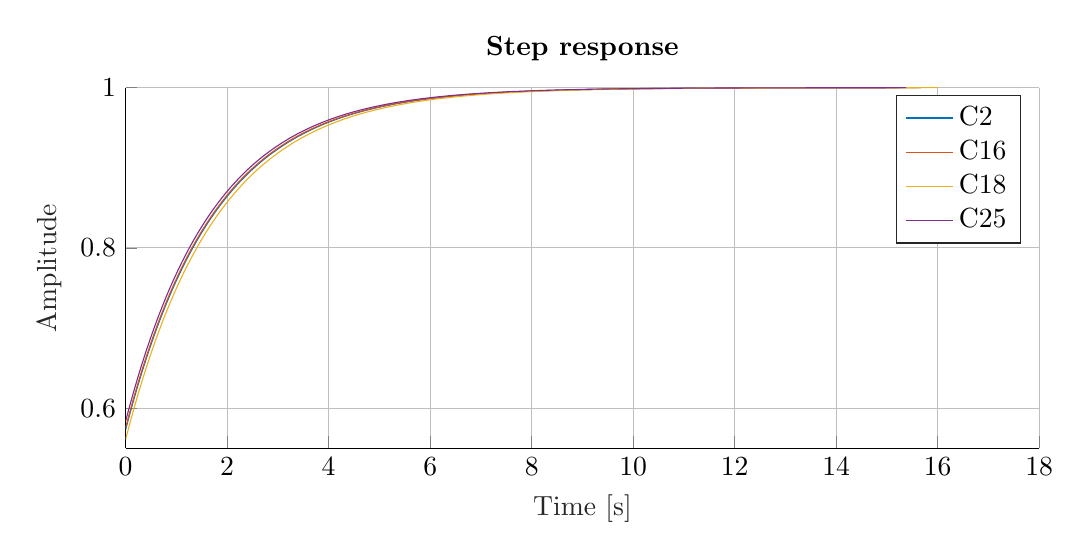
\begin{tikzpicture}

\begin{axis}[%
width=4.568in,
height=1.803in,
at={(0.766in,0.486in)},
scale only axis,
xmin=0,
xmax=18,
xlabel style={font=\color{white!15!black}},
xlabel={Time [s]},
ymin=0.55,
ymax=1,
ylabel style={font=\color{white!15!black}},
ylabel={Amplitude},
axis background/.style={fill=white},
title style={font=\bfseries},
title={Step response},
axis x line*=bottom,
axis y line*=left,
xmajorgrids,
ymajorgrids,
legend style={legend cell align=left, align=left, draw=white!15!black}
]
\addplot [color=mycolor1]
  table[row sep=crcr]{%
0	0.573149389176775\\
0.0803485142433953	0.592360831325092\\
0.160697028486789	0.610707616143515\\
0.241045542730184	0.628228659622438\\
0.321394056973578	0.644961126244171\\
0.401742571216973	0.660940507813777\\
0.482091085460368	0.676200698741958\\
0.562439599703762	0.690774067939643\\
0.642788113947157	0.704691527476786\\
0.72313662819055	0.717982598151011\\
0.803485142433946	0.730675472105181\\
0.883833656677341	0.74279707262672\\
0.964182170920735	0.754373111255504\\
1.04453068516413	0.76542814232149\\
1.12487919940752	0.775985615027745\\
1.20522771365092	0.786067923189339\\
1.28557622789431	0.795696452733647\\
1.36592474213771	0.80489162706275\\
1.4462732563811	0.813672950374217\\
1.5266217706245	0.822059049032127\\
1.60697028486789	0.830067711076074\\
1.68731879911129	0.837715923951995\\
1.76766731335468	0.845019910544814\\
1.84801582759808	0.851995163589356\\
1.92836434184147	0.858656478532517\\
2.00871285608486	0.865017984916388\\
2.08906137032826	0.871093176348916\\
2.16940988457165	0.87689493912564\\
2.24975839881505	0.882435579563266\\
2.33010691305844	0.887726850103011\\
2.41045542730184	0.892779974239099\\
2.49080394154523	0.89760567032531\\
2.57115245578863	0.902214174310036\\
2.65150097003202	0.906615261448097\\
2.73184948427542	0.910818267035381\\
2.81219799851881	0.914832106210245\\
2.89254651276221	0.918665292863722\\
3.05324354124899	0.925821865475871\\
3.21394056973578	0.932348737270793\\
3.37463759822257	0.938301315094845\\
3.53533462670936	0.943730130592492\\
3.69603165519615	0.94868126917121\\
3.85672868368294	0.953196761222154\\
4.01742571216973	0.957314938917639\\
4.17812274065652	0.961070761614318\\
4.33881976914331	0.964496112624385\\
4.4995167976301	0.967620069874167\\
4.66021382611689	0.970469152747652\\
4.82091085460367	0.973067547210494\\
5.06195639733386	0.976542814232129\\
5.30300194006404	0.979569645273347\\
5.54404748279423	0.982205904903196\\
5.78509302552441	0.984501991054467\\
6.02613856825459	0.986501798491627\\
6.34753262522817	0.988772685010291\\
6.66892668220175	0.990661526144802\\
6.99032073917533	0.992232595769856\\
7.3920633103923	0.99383013150948\\
7.79380588160928	0.995099099253443\\
8.27589696706964	0.996282286596218\\
8.8383365667734	0.997306754721047\\
9.48112468072056	0.998136729503738\\
10.2846098231545	0.99882435579563\\
11.3291405083186	0.999353935456584\\
12.7754137646997	0.999717982598151\\
15.1858691920016	0.999929160431485\\
15.6679602774619	0.9999462626919\\
};
\addlegendentry{C2}

\addplot [color=mycolor2]
  table[row sep=crcr]{%
0	0.575667051395207\\
0.0799971124771695	0.5947651800778\\
0.159994224954341	0.61300375137656\\
0.23999133743151	0.6304214517465\\
0.31998844990868	0.647055226465337\\
0.399985562385851	0.662940357999375\\
0.47998267486302	0.678110540842358\\
0.55997978734019	0.692597952985997\\
0.639976899817359	0.706433324173808\\
0.71997401229453	0.719646001083024\\
0.7999711247717	0.732264009572821\\
0.879968237248869	0.744314114130933\\
0.959965349726041	0.755821874644715\\
1.03996246220321	0.766811700617085\\
1.11995957468038	0.777306902942366\\
1.19995668715755	0.787329743351803\\
1.27995379963472	0.796901481633693\\
1.35995091211189	0.806042420728234\\
1.43994802458906	0.814771949792796\\
1.51994513706623	0.82310858532891\\
1.5999422495434	0.831070010458264\\
1.67993936202057	0.838673112430961\\
1.75993647449774	0.84593401844565\\
1.83993358697491	0.852868129857479\\
1.91993069945208	0.859490154846421\\
1.99992781192925	0.86581413961531\\
2.07992492440642	0.871853498183711\\
2.15992203688359	0.877621040840859\\
2.23991914936076	0.883129001317998\\
2.31991626183793	0.888389062737765\\
2.3999133743151	0.89341238239566\\
2.47991048679227	0.898209615426165\\
2.55990759926944	0.902790937403715\\
2.63990471174661	0.907166065926454\\
2.71990182422378	0.911344281228558\\
2.79989893670095	0.91533444586487\\
2.87989604917812	0.919145023509554\\
3.03989027413246	0.926259385024842\\
3.1998844990868	0.932747759841883\\
3.35987872404114	0.938665228004828\\
3.51987294899548	0.944062023110979\\
3.67986717394982	0.94898395874557\\
3.83986139890416	0.95347281739493\\
3.9998556238585	0.957566705139483\\
4.15984984881284	0.961300375137622\\
4.31984407376718	0.964705522646502\\
4.47983829872152	0.967811054084207\\
4.63983252367586	0.970643332417355\\
4.7998267486302	0.973226400957259\\
5.03981808606171	0.976681170061688\\
5.27980942349322	0.979690148163352\\
5.51980076092473	0.982310858532875\\
5.75979209835624	0.984593401844551\\
5.99978343578775	0.986581413961519\\
6.31977188569643	0.988838906273767\\
6.63976033560511	0.990716606592636\\
6.95974878551379	0.992278409690861\\
7.35973434789964	0.993866522800477\\
7.75971991028549	0.99512800588338\\
8.23970258514851	0.996304214517458\\
8.7996823724887	0.997322640095723\\
9.43965927230606	0.998147719497924\\
10.2396303970778	0.998831290013177\\
11.279592859281	0.999357746092555\\
12.71954088387	0.999719646001083\\
15.1194542581851	0.99992957825941\\
15.5994369330481	0.999946579646794\\
};
\addlegendentry{C16}

\addplot [color=mycolor3]
  table[row sep=crcr]{%
0	0.561043487421703\\
0.0820822322909329	0.580799784901892\\
0.164164464581866	0.59966690252271\\
0.246246696872795	0.617684859970183\\
0.328328929163728	0.634891875747769\\
0.410411161454661	0.651324448242921\\
0.492493393745594	0.667017433145052\\
0.574575626036523	0.68200411737913\\
0.656657858327456	0.696316289711721\\
0.738740090618389	0.709984308179205\\
0.820822322909322	0.723037164481259\\
0.902904555200251	0.735502545476123\\
0.984986787491184	0.747406891908152\\
1.06706901978212	0.75877545449217\\
1.14915125207305	0.769632347473628\\
1.23123348436398	0.780000599778148\\
1.31331571665491	0.789902203858965\\
1.39539794894585	0.799358162345865\\
1.47748018123678	0.808388532594581\\
1.55956241352771	0.817012469231134\\
1.64164464581864	0.825248264781358\\
1.72372687810957	0.833113388471816\\
1.80580911040051	0.84062452328434\\
1.88789134269144	0.847797601342911\\
1.96997357498237	0.854647837707798\\
2.0520558072733	0.86118976264876\\
2.13413803956423	0.867437252465688\\
2.21622027185516	0.873403558922096\\
2.2983025041461	0.879101337353902\\
2.38038473643703	0.884542673513067\\
2.46246696872796	0.88973910920312\\
2.54454920101889	0.894701666760859\\
2.62663143330983	0.899440872436205\\
2.70871366560076	0.903966778719788\\
2.79079589789169	0.908288985665642\\
2.87287813018262	0.912416661254181\\
2.95496036247355	0.916358560838738\\
3.11912482705542	0.923718100865596\\
3.28328929163728	0.930430081142767\\
3.44745375621915	0.936551479909092\\
3.61161822080101	0.942134261935998\\
3.77578268538288	0.947225819658296\\
3.93994714996474	0.951869375490244\\
4.1041116145466	0.95610434874213\\
4.26827607912847	0.959966690252234\\
4.43244054371033	0.963489187574744\\
4.59660500829219	0.966701743314474\\
4.76076947287406	0.969631628971143\\
4.92493393745592	0.972303716448099\\
5.17118063432872	0.975877545449194\\
5.41742733120152	0.978990220385878\\
5.66367402807431	0.981701246923095\\
5.90992072494711	0.98406245232842\\
6.15616742181991	0.986118976264862\\
6.48449635098363	0.988454267351297\\
6.81282528014736	0.990396677871971\\
7.14115420931109	0.992012304571674\\
7.55156537076575	0.993655147990903\\
7.96197653222041	0.994960104904028\\
8.454469925966	0.996176848599696\\
9.02904555200253	0.997230371644807\\
9.68570341032998	0.998083885325943\\
10.5065257332393	0.998791013373538\\
11.5735947530214	0.999335612432812\\
13.0510749342582	0.999709984308179\\
15.4314596706952	0.999923718100867\\
16.0060352967317	0.999944738649162\\
};
\addlegendentry{C18}

\addplot [color=mycolor4]
  table[row sep=crcr]{%
0	0.583891612087116\\
0.0788702918599089	0.602619574561858\\
0.157740583719818	0.620504639876524\\
0.236610875579725	0.637584744652539\\
0.315481167439634	0.653896118082102\\
0.394351459299543	0.669473358775164\\
0.473221751159452	0.684349508147708\\
0.552092043019361	0.698556120507037\\
0.630962334879269	0.712123329982676\\
0.709832626739177	0.725079914444912\\
0.788702918599085	0.737453356546506\\
0.867573210458994	0.749269902017096\\
0.946443502318903	0.760554615333895\\
1.02531379417881	0.771331432886814\\
1.10418408603872	0.781623213750759\\
1.18305437789863	0.791451788172782\\
1.26192466975854	0.800838003876976\\
1.34079496161845	0.809801770285279\\
1.41966525347835	0.818362100748036\\
1.49853554533826	0.826537152873863\\
1.57740583719817	0.834344267044367\\
1.65627612905808	0.84180000319542\\
1.73514642091799	0.848920175943009\\
1.8140167127779	0.855719888128148\\
1.89288700463781	0.862213562852036\\
1.97175729649772	0.868414974069383\\
2.05062758835762	0.874337275804821\\
2.12949788021753	0.879993030054345\\
2.20836817207744	0.885394233431001\\
2.28723846393735	0.890552342611301\\
2.36610875579726	0.895478298636375\\
2.44497904765717	0.900182550119389\\
2.52384933951708	0.90467507540845\\
2.60271963137698	0.908965403752015\\
2.68158992323689	0.913062635511718\\
2.7604602150968	0.916975461465446\\
2.91820079881662	0.924280720923962\\
3.07594138253643	0.930943196734436\\
3.23368196625625	0.937019446890535\\
3.39142254997607	0.942561052895535\\
3.54916313369589	0.947615057639535\\
3.7069037174157	0.95222436474822\\
3.86464430113552	0.956428102793261\\
4.02238488485534	0.960261957456151\\
4.18012546857516	0.963758474465221\\
4.33786605229497	0.966947335877487\\
4.49560663601479	0.969855612050678\\
4.65334721973461	0.972507991444466\\
4.88995809531433	0.976055461533369\\
5.12656897089406	0.97914517881726\\
5.36317984647379	0.981836210074787\\
5.59979072205351	0.984180000319528\\
5.83640159763324	0.986221356285192\\
6.15188276507287	0.98853942334309\\
6.46736393251251	0.990467507540837\\
6.78284509995214	0.992071218124158\\
7.17719655925168	0.993701944689048\\
7.57154801855123	0.994997276842655\\
8.04476976971068	0.996205046398758\\
8.59686181273004	0.997250799144444\\
9.22782414760931	0.99809801770285\\
10.0165270662084	0.998799930300541\\
11.0418408603872	0.999340512648669\\
12.4615061138656	0.999712123329981\\
14.7487445778029	0.999924280720924\\
15.3797069126822	0.999947615057639\\
};
\addlegendentry{C25}

\end{axis}
\end{tikzpicture}%
\caption{Closed loop step response of the PI controllers and models.}
\label{fig:Tikz_PI_PUMP_GAIN}
\end{figure}



The PI controller are implemented on the water system described in \chapref{system_overview} and tested. In \figref{fig:Tikz_PI_PUMP_GAINNNN} the step response of the pumps can be seen. The system is starting in a steady state position of 0.15 bars and is then giving a step increase of 0.15 bars to each pump at different times. It can be seen that the pumps have some small deviations compared to the desired steady state value. This is however deemed sufficient, since the largest deviations are between $\pm 1.5$ [mbar].

\begin{figure}[H]
\centering
% This file was created by matlab2tikz.
%
%The latest updates can be retrieved from
%  http://www.mathworks.com/matlabcentral/fileexchange/22022-matlab2tikz-matlab2tikz
%where you can also make suggestions and rate matlab2tikz.
%
\definecolor{mycolor1}{rgb}{1.00000,1.00000,0.00000}%
%
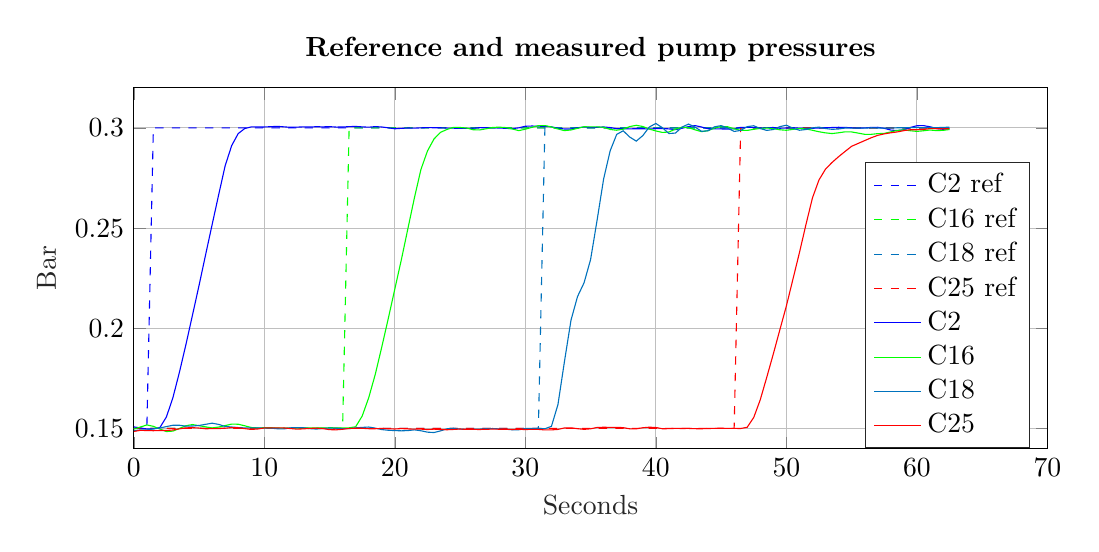
\begin{tikzpicture}

\begin{axis}[%
width=4.568in,
height=1.803in,
at={(0.758in,0.481in)},
scale only axis,
xmin=0,
xmax=70,
xlabel style={font=\color{white!15!black}},
xlabel={Seconds},
ymin=0.14,
ymax=0.32,
ylabel style={font=\color{white!15!black}},
ylabel={Bar},
axis background/.style={fill=white},
title style={font=\bfseries},
title={Reference and measured pump pressures},
xmajorgrids,
ymajorgrids,
legend style={at={(0.8,0)}, anchor=south west, legend cell align=left, align=left, draw=white!15!black}
]
\addplot [color=blue, dashed]
  table[row sep=crcr]{%
0	0.15\\
0.5	0.15\\
1	0.15\\
1.5	0.3\\
2	0.3\\
2.5	0.3\\
3	0.3\\
3.5	0.3\\
4	0.3\\
4.5	0.3\\
5	0.3\\
5.5	0.3\\
6	0.3\\
6.5	0.3\\
7	0.3\\
7.5	0.3\\
8	0.3\\
8.5	0.3\\
9	0.3\\
9.5	0.3\\
10	0.3\\
10.5	0.3\\
11	0.3\\
11.5	0.3\\
12	0.3\\
12.5	0.3\\
13	0.3\\
13.5	0.3\\
14	0.3\\
14.5	0.3\\
15	0.3\\
15.5	0.3\\
16	0.3\\
16.5	0.3\\
17	0.3\\
17.5	0.3\\
18	0.3\\
18.5	0.3\\
19	0.3\\
19.5	0.3\\
20	0.3\\
20.5	0.3\\
21	0.3\\
21.5	0.3\\
22	0.3\\
22.5	0.3\\
23	0.3\\
23.5	0.3\\
24	0.3\\
24.5	0.3\\
25	0.3\\
25.5	0.3\\
26	0.3\\
26.5	0.3\\
27	0.3\\
27.5	0.3\\
28	0.3\\
28.5	0.3\\
29	0.3\\
29.5	0.3\\
30	0.3\\
30.5	0.3\\
31	0.3\\
31.5	0.3\\
32	0.3\\
32.5	0.3\\
33	0.3\\
33.5	0.3\\
34	0.3\\
34.5	0.3\\
35	0.3\\
35.5	0.3\\
36	0.3\\
36.5	0.3\\
37	0.3\\
37.5	0.3\\
38	0.3\\
38.5	0.3\\
39	0.3\\
39.5	0.3\\
40	0.3\\
40.5	0.3\\
41	0.3\\
41.5	0.3\\
42	0.3\\
42.5	0.3\\
43	0.3\\
43.5	0.3\\
44	0.3\\
44.5	0.3\\
45	0.3\\
45.5	0.3\\
46	0.3\\
46.5	0.3\\
47	0.3\\
47.5	0.3\\
48	0.3\\
48.5	0.3\\
49	0.3\\
49.5	0.3\\
50	0.3\\
50.5	0.3\\
51	0.3\\
51.5	0.3\\
52	0.3\\
52.5	0.3\\
53	0.3\\
53.5	0.3\\
54	0.3\\
54.5	0.3\\
55	0.3\\
55.5	0.3\\
56	0.3\\
56.5	0.3\\
57	0.3\\
57.5	0.3\\
58	0.3\\
58.5	0.3\\
59	0.3\\
59.5	0.3\\
60	0.3\\
60.5	0.3\\
61	0.3\\
61.5	0.3\\
62	0.3\\
62.5	0.3\\
};
\addlegendentry{C2 ref}

\addplot [color=green, dashed]
  table[row sep=crcr]{%
0	0.15\\
0.5	0.15\\
1	0.15\\
1.5	0.15\\
2	0.15\\
2.5	0.15\\
3	0.15\\
3.5	0.15\\
4	0.15\\
4.5	0.15\\
5	0.15\\
5.5	0.15\\
6	0.15\\
6.5	0.15\\
7	0.15\\
7.5	0.15\\
8	0.15\\
8.5	0.15\\
9	0.15\\
9.5	0.15\\
10	0.15\\
10.5	0.15\\
11	0.15\\
11.5	0.15\\
12	0.15\\
12.5	0.15\\
13	0.15\\
13.5	0.15\\
14	0.15\\
14.5	0.15\\
15	0.15\\
15.5	0.15\\
16	0.15\\
16.5	0.3\\
17	0.3\\
17.5	0.3\\
18	0.3\\
18.5	0.3\\
19	0.3\\
19.5	0.3\\
20	0.3\\
20.5	0.3\\
21	0.3\\
21.5	0.3\\
22	0.3\\
22.5	0.3\\
23	0.3\\
23.5	0.3\\
24	0.3\\
24.5	0.3\\
25	0.3\\
25.5	0.3\\
26	0.3\\
26.5	0.3\\
27	0.3\\
27.5	0.3\\
28	0.3\\
28.5	0.3\\
29	0.3\\
29.5	0.3\\
30	0.3\\
30.5	0.3\\
31	0.3\\
31.5	0.3\\
32	0.3\\
32.5	0.3\\
33	0.3\\
33.5	0.3\\
34	0.3\\
34.5	0.3\\
35	0.3\\
35.5	0.3\\
36	0.3\\
36.5	0.3\\
37	0.3\\
37.5	0.3\\
38	0.3\\
38.5	0.3\\
39	0.3\\
39.5	0.3\\
40	0.3\\
40.5	0.3\\
41	0.3\\
41.5	0.3\\
42	0.3\\
42.5	0.3\\
43	0.3\\
43.5	0.3\\
44	0.3\\
44.5	0.3\\
45	0.3\\
45.5	0.3\\
46	0.3\\
46.5	0.3\\
47	0.3\\
47.5	0.3\\
48	0.3\\
48.5	0.3\\
49	0.3\\
49.5	0.3\\
50	0.3\\
50.5	0.3\\
51	0.3\\
51.5	0.3\\
52	0.3\\
52.5	0.3\\
53	0.3\\
53.5	0.3\\
54	0.3\\
54.5	0.3\\
55	0.3\\
55.5	0.3\\
56	0.3\\
56.5	0.3\\
57	0.3\\
57.5	0.3\\
58	0.3\\
58.5	0.3\\
59	0.3\\
59.5	0.3\\
60	0.3\\
60.5	0.3\\
61	0.3\\
61.5	0.3\\
62	0.3\\
62.5	0.3\\
};
\addlegendentry{C16 ref}

\addplot [color=mycolor1, dashed]
  table[row sep=crcr]{%
0	0.15\\
0.5	0.15\\
1	0.15\\
1.5	0.15\\
2	0.15\\
2.5	0.15\\
3	0.15\\
3.5	0.15\\
4	0.15\\
4.5	0.15\\
5	0.15\\
5.5	0.15\\
6	0.15\\
6.5	0.15\\
7	0.15\\
7.5	0.15\\
8	0.15\\
8.5	0.15\\
9	0.15\\
9.5	0.15\\
10	0.15\\
10.5	0.15\\
11	0.15\\
11.5	0.15\\
12	0.15\\
12.5	0.15\\
13	0.15\\
13.5	0.15\\
14	0.15\\
14.5	0.15\\
15	0.15\\
15.5	0.15\\
16	0.15\\
16.5	0.15\\
17	0.15\\
17.5	0.15\\
18	0.15\\
18.5	0.15\\
19	0.15\\
19.5	0.15\\
20	0.15\\
20.5	0.15\\
21	0.15\\
21.5	0.15\\
22	0.15\\
22.5	0.15\\
23	0.15\\
23.5	0.15\\
24	0.15\\
24.5	0.15\\
25	0.15\\
25.5	0.15\\
26	0.15\\
26.5	0.15\\
27	0.15\\
27.5	0.15\\
28	0.15\\
28.5	0.15\\
29	0.15\\
29.5	0.15\\
30	0.15\\
30.5	0.15\\
31	0.15\\
31.5	0.3\\
32	0.3\\
32.5	0.3\\
33	0.3\\
33.5	0.3\\
34	0.3\\
34.5	0.3\\
35	0.3\\
35.5	0.3\\
36	0.3\\
36.5	0.3\\
37	0.3\\
37.5	0.3\\
38	0.3\\
38.5	0.3\\
39	0.3\\
39.5	0.3\\
40	0.3\\
40.5	0.3\\
41	0.3\\
41.5	0.3\\
42	0.3\\
42.5	0.3\\
43	0.3\\
43.5	0.3\\
44	0.3\\
44.5	0.3\\
45	0.3\\
45.5	0.3\\
46	0.3\\
46.5	0.3\\
47	0.3\\
47.5	0.3\\
48	0.3\\
48.5	0.3\\
49	0.3\\
49.5	0.3\\
50	0.3\\
50.5	0.3\\
51	0.3\\
51.5	0.3\\
52	0.3\\
52.5	0.3\\
53	0.3\\
53.5	0.3\\
54	0.3\\
54.5	0.3\\
55	0.3\\
55.5	0.3\\
56	0.3\\
56.5	0.3\\
57	0.3\\
57.5	0.3\\
58	0.3\\
58.5	0.3\\
59	0.3\\
59.5	0.3\\
60	0.3\\
60.5	0.3\\
61	0.3\\
61.5	0.3\\
62	0.3\\
62.5	0.3\\
};
\addlegendentry{C18 ref}

\addplot [color=red, dashed]
  table[row sep=crcr]{%
0	0.15\\
0.5	0.15\\
1	0.15\\
1.5	0.15\\
2	0.15\\
2.5	0.15\\
3	0.15\\
3.5	0.15\\
4	0.15\\
4.5	0.15\\
5	0.15\\
5.5	0.15\\
6	0.15\\
6.5	0.15\\
7	0.15\\
7.5	0.15\\
8	0.15\\
8.5	0.15\\
9	0.15\\
9.5	0.15\\
10	0.15\\
10.5	0.15\\
11	0.15\\
11.5	0.15\\
12	0.15\\
12.5	0.15\\
13	0.15\\
13.5	0.15\\
14	0.15\\
14.5	0.15\\
15	0.15\\
15.5	0.15\\
16	0.15\\
16.5	0.15\\
17	0.15\\
17.5	0.15\\
18	0.15\\
18.5	0.15\\
19	0.15\\
19.5	0.15\\
20	0.15\\
20.5	0.15\\
21	0.15\\
21.5	0.15\\
22	0.15\\
22.5	0.15\\
23	0.15\\
23.5	0.15\\
24	0.15\\
24.5	0.15\\
25	0.15\\
25.5	0.15\\
26	0.15\\
26.5	0.15\\
27	0.15\\
27.5	0.15\\
28	0.15\\
28.5	0.15\\
29	0.15\\
29.5	0.15\\
30	0.15\\
30.5	0.15\\
31	0.15\\
31.5	0.15\\
32	0.15\\
32.5	0.15\\
33	0.15\\
33.5	0.15\\
34	0.15\\
34.5	0.15\\
35	0.15\\
35.5	0.15\\
36	0.15\\
36.5	0.15\\
37	0.15\\
37.5	0.15\\
38	0.15\\
38.5	0.15\\
39	0.15\\
39.5	0.15\\
40	0.15\\
40.5	0.15\\
41	0.15\\
41.5	0.15\\
42	0.15\\
42.5	0.15\\
43	0.15\\
43.5	0.15\\
44	0.15\\
44.5	0.15\\
45	0.15\\
45.5	0.15\\
46	0.15\\
46.5	0.3\\
47	0.3\\
47.5	0.3\\
48	0.3\\
48.5	0.3\\
49	0.3\\
49.5	0.3\\
50	0.3\\
50.5	0.3\\
51	0.3\\
51.5	0.3\\
52	0.3\\
52.5	0.3\\
53	0.3\\
53.5	0.3\\
54	0.3\\
54.5	0.3\\
55	0.3\\
55.5	0.3\\
56	0.3\\
56.5	0.3\\
57	0.3\\
57.5	0.3\\
58	0.3\\
58.5	0.3\\
59	0.3\\
59.5	0.3\\
60	0.3\\
60.5	0.3\\
61	0.3\\
61.5	0.3\\
62	0.3\\
62.5	0.3\\
};
\addlegendentry{C25 ref}

\addplot [color=blue]
  table[row sep=crcr]{%
0	0.15078201368524\\
0.5	0.150244379276638\\
1	0.149737292277615\\
1.5	0.149792277614859\\
2	0.150433773216032\\
2.5	0.155730694037146\\
3	0.165414222873901\\
3.5	0.178115835777127\\
4	0.192014907135875\\
4.5	0.206653225806451\\
5	0.221370967741934\\
5.5	0.236614125122188\\
6	0.2516495601173\\
6.5	0.266526148582598\\
7	0.281091153470183\\
7.5	0.291165689149558\\
8	0.297177419354836\\
8.5	0.299700635386116\\
9	0.300507086999019\\
9.5	0.300519305962851\\
10	0.300482649071356\\
10.5	0.30062927663734\\
11	0.300788123167156\\
11.5	0.300549853372436\\
12	0.300317693059632\\
12.5	0.300409335288371\\
13	0.300525415444775\\
13.5	0.300507086999029\\
14	0.30059872922777\\
14.5	0.300543743890528\\
15	0.300641495601184\\
15.5	0.300433773216042\\
16	0.300464320625622\\
16.5	0.300653714565016\\
17	0.300751466275671\\
17.5	0.300531524926697\\
18	0.300372678396883\\
18.5	0.300659824046932\\
19	0.300476539589454\\
19.5	0.300067204301086\\
20	0.299584555229726\\
20.5	0.299792277614868\\
21	0.299963343108514\\
21.5	0.299896138807439\\
22	0.300042766373421\\
22.5	0.300183284457487\\
23	0.300091642228749\\
23.5	0.300085532746832\\
24	0.299945014662766\\
24.5	0.299877810361692\\
25	0.299822825024449\\
25.5	0.299773949169122\\
26	0.299859481915945\\
26.5	0.300128299120246\\
27	0.300103861192582\\
27.5	0.300018328445759\\
28	0.299981671554263\\
28.5	0.29979227761487\\
29	0.299651759530803\\
29.5	0.300061094819171\\
30	0.300843108504409\\
30.5	0.300953079178896\\
31	0.300898093841653\\
31.5	0.300788123167166\\
32	0.300568181818193\\
32.5	0.299841153470197\\
33	0.299474584555242\\
33.5	0.299480694037157\\
34	0.30009164222875\\
34.5	0.30045210166179\\
35	0.30028714565006\\
35.5	0.300323802541556\\
36	0.30048264907137\\
36.5	0.300195503421321\\
37	0.299615102639308\\
37.5	0.299578445747812\\
38	0.299535679374401\\
38.5	0.299621212121224\\
39	0.299602883675476\\
39.5	0.299499022482905\\
40	0.29962732160314\\
40.5	0.299725073313795\\
41	0.299535679374401\\
41.5	0.299144672531781\\
42	0.299822825024449\\
42.5	0.300659824046932\\
43	0.30117302052787\\
43.5	0.300470430107538\\
44	0.29959677419356\\
44.5	0.299584555229728\\
45	0.299511241446737\\
45.5	0.299407380254166\\
46	0.299547898338233\\
46.5	0.300305474095808\\
47	0.300311583577724\\
47.5	0.300262707722396\\
48	0.300006109481927\\
48.5	0.300140518084078\\
49	0.300207722385153\\
49.5	0.299853372434029\\
50	0.2999572336266\\
50.5	0.300097751710666\\
51	0.29989613880744\\
51.5	0.29976173020529\\
52	0.299835043988281\\
52.5	0.299963343108515\\
53	0.300171065493657\\
53.5	0.300195503421321\\
54	0.300323802541555\\
54.5	0.300262707722396\\
55	0.300073313783003\\
55.5	0.299945014662768\\
56	0.300006109481927\\
56.5	0.300250488758564\\
57	0.30031769305964\\
57.5	0.299804496578702\\
58	0.298949169110472\\
58.5	0.298674242424255\\
59	0.299114125122202\\
59.5	0.300238269794733\\
60	0.301099706744878\\
60.5	0.301166911045954\\
61	0.300592619745856\\
61.5	0.299737292277626\\
62	0.299327956989259\\
62.5	0.299584555229728\\
};
\addlegendentry{C2}

\addplot [color=green]
  table[row sep=crcr]{%
0	0.149676197458456\\
0.5	0.150696480938417\\
1	0.151753421309873\\
1.5	0.151050830889541\\
2	0.1497311827957\\
2.5	0.148435972629522\\
3	0.148674242424243\\
3.5	0.150006109481917\\
4	0.151362414467253\\
4.5	0.151936705767352\\
5	0.151380742913002\\
5.5	0.150788123167157\\
6	0.150287145650051\\
6.5	0.150684261974587\\
7	0.151423509286415\\
7.5	0.15216886608016\\
8	0.152101661779085\\
8.5	0.151325757575762\\
9	0.1504582111437\\
9.5	0.150268817204306\\
10	0.150348240469214\\
10.5	0.150348240469214\\
11	0.150226050830895\\
11.5	0.150134408602156\\
12	0.150085532746829\\
12.5	0.150226050830895\\
13	0.150201612903231\\
13.5	0.150244379276643\\
14	0.150226050830895\\
14.5	0.150256598240475\\
15	0.150336021505382\\
15.5	0.150299364613886\\
16	0.150287145650054\\
16.5	0.150305474095802\\
17	0.150836999022488\\
17.5	0.156176686217014\\
18	0.165322580645165\\
18.5	0.176930596285439\\
19	0.190603616813296\\
19.5	0.204887585532748\\
20	0.219568670576737\\
20.5	0.234176441837734\\
21	0.249663978494626\\
21.5	0.265053763440863\\
22	0.279233870967746\\
22.5	0.288465298142722\\
23	0.29446480938417\\
23.5	0.297794477028355\\
24	0.299260752688181\\
24.5	0.300311583577723\\
25	0.300219941348984\\
25.5	0.299981671554261\\
26	0.299108015640283\\
26.5	0.298998044965796\\
27	0.299590664711642\\
27.5	0.30023826979473\\
28	0.300391006842628\\
28.5	0.30017717497557\\
29	0.299480694037153\\
29.5	0.298655913978502\\
30	0.299370723362666\\
30.5	0.300293255131973\\
31	0.301142473118287\\
31.5	0.301179130009783\\
32	0.300507086999031\\
32.5	0.299486803519071\\
33	0.29866202346042\\
33.5	0.298998044965797\\
34	0.299816715542533\\
34.5	0.300610948191604\\
35	0.300500977517117\\
35.5	0.300513196480949\\
36	0.300342130987303\\
36.5	0.299242424242436\\
37	0.298851417399817\\
37.5	0.299395161290335\\
38	0.300690371456511\\
38.5	0.301313538611936\\
39	0.300727028348007\\
39.5	0.299425708699914\\
40	0.298503176930609\\
40.5	0.297757820136866\\
41	0.297959433040091\\
41.5	0.29940127077225\\
42	0.300391006842631\\
42.5	0.300158846529826\\
43	0.299083577712622\\
43.5	0.298136608015653\\
44	0.298637585532759\\
44.5	0.299951124144684\\
45	0.300745356793755\\
45.5	0.30058651026394\\
46	0.299560117302065\\
46.5	0.298790322580658\\
47	0.298753665689162\\
47.5	0.299321847507343\\
48	0.299743401759542\\
48.5	0.299975562072348\\
49	0.299651759530803\\
49.5	0.299089687194538\\
50	0.298833088954069\\
50.5	0.299285190615848\\
51	0.299663978494635\\
51.5	0.299523460410569\\
52	0.298833088954069\\
52.5	0.298093841642242\\
53	0.297543988269808\\
53.5	0.297183528836769\\
54	0.297580645161304\\
54.5	0.298063294232662\\
55	0.298002199413503\\
55.5	0.297427908113406\\
56	0.296816959921813\\
56.5	0.296810850439897\\
57	0.297152981427189\\
57.5	0.297281280547423\\
58	0.298020527859251\\
58.5	0.29877199413491\\
59	0.299004154447715\\
59.5	0.298594819159348\\
60	0.298283235581636\\
60.5	0.298588709677432\\
61	0.298955278592388\\
61.5	0.298674242424255\\
62	0.298790322580658\\
62.5	0.299211876832857\\
};
\addlegendentry{C16}

\addplot [color=mycolor1]
  table[row sep=crcr]{%
0	0.148930840664711\\
0.5	0.14924853372434\\
1	0.149242424242424\\
1.5	0.149767839687194\\
2	0.150213831867058\\
2.5	0.150922531769307\\
3	0.151600684261975\\
3.5	0.151594574780059\\
4	0.151118035190617\\
4.5	0.151215786901272\\
5	0.151472385141742\\
5.5	0.152052785923756\\
6	0.152620967741938\\
6.5	0.152022238514176\\
7	0.151001955034215\\
7.5	0.150720918866082\\
8	0.150439882697949\\
8.5	0.150262707722387\\
9	0.150293255131967\\
9.5	0.150232160312808\\
10	0.150158846529816\\
10.5	0.150158846529816\\
11	0.149841153470188\\
11.5	0.149755620723365\\
12	0.150305474095799\\
12.5	0.15040933528837\\
13	0.150329912023463\\
13.5	0.149896138807432\\
14	0.14968841642229\\
14.5	0.150006109481918\\
15	0.15021383186706\\
15.5	0.150122189638321\\
16	0.149883919843599\\
16.5	0.149883919843601\\
17	0.150299364613884\\
17.5	0.150519305962858\\
18	0.150702590420336\\
18.5	0.150146627565987\\
19	0.149437927663739\\
19.5	0.149095796676447\\
20	0.148930840664717\\
20.5	0.148808651026399\\
21	0.148936950146633\\
21.5	0.149285190615841\\
22	0.148845307917894\\
22.5	0.148148826979478\\
23	0.147953323558169\\
23.5	0.148778103616819\\
24	0.149810606060612\\
24.5	0.150091642228745\\
25	0.14966397849463\\
25.5	0.1494990224829\\
26	0.149572336265891\\
26.5	0.149676197458462\\
27	0.149847262952107\\
27.5	0.149951124144678\\
28	0.1497678396872\\
28.5	0.149608993157386\\
29	0.149321847507338\\
29.5	0.149340175953085\\
30	0.149938905180846\\
30.5	0.150024437927669\\
31	0.150079423264913\\
31.5	0.149847262952107\\
32	0.15104472140763\\
32.5	0.161907380254158\\
33	0.183479960899319\\
33.5	0.204056695992182\\
34	0.215835777126101\\
34.5	0.222690615835779\\
35	0.234292521994136\\
35.5	0.253971163245356\\
36	0.274560117302051\\
36.5	0.288563049853369\\
37	0.296774193548383\\
37.5	0.298576490713585\\
38	0.295460654936456\\
38.5	0.293426197458449\\
39	0.296157135874871\\
39.5	0.300464320625601\\
40	0.302248289345056\\
40.5	0.300109970674479\\
41	0.297220185728242\\
41.5	0.2974340175953\\
42	0.300354349951117\\
42.5	0.301942815249262\\
43	0.300452101661775\\
43.5	0.2983137829912\\
44	0.298588709677419\\
44.5	0.300568181818187\\
45	0.3011485826002\\
45.5	0.299957233626594\\
46	0.298246578690134\\
46.5	0.298778103616822\\
47	0.300635386119268\\
47.5	0.301093597262962\\
48	0.299700635386131\\
48.5	0.29877199413491\\
49	0.299205767350941\\
49.5	0.3006476050831\\
50	0.301368523949179\\
50.5	0.299883919843609\\
51	0.298845307917901\\
51.5	0.299205767350941\\
52	0.300030547409591\\
52.5	0.300415444770294\\
53	0.299700635386131\\
53.5	0.299321847507343\\
54	0.299468475073326\\
54.5	0.299963343108516\\
55	0.299896138807441\\
55.5	0.299963343108516\\
56	0.299896138807441\\
56.5	0.300079423264918\\
57	0.299969452590432\\
57.5	0.299914467253188\\
58	0.300012218963843\\
58.5	0.300073313783003\\
59	0.300097751710666\\
59.5	0.300134408602162\\
60	0.300189393939405\\
60.5	0.300128299120246\\
61	0.300232160312817\\
61.5	0.30012218963833\\
62	0.300281036168144\\
62.5	0.300360459433051\\
};
\addlegendentry{C18}

\addplot [color=red]
  table[row sep=crcr]{%
0	0.148490957966764\\
0.5	0.14905303030303\\
1	0.148955278592375\\
1.5	0.148863636363635\\
2	0.148967497556206\\
2.5	0.148985826001954\\
3	0.14921798631476\\
3.5	0.149810606060605\\
4	0.150287145650049\\
4.5	0.15039100684262\\
5	0.150201612903227\\
5.5	0.149828934506356\\
6	0.149926686217011\\
6.5	0.149938905180844\\
7	0.150103861192575\\
7.5	0.150445992179868\\
8	0.150342130987297\\
8.5	0.149908357771266\\
9	0.149511241446731\\
9.5	0.149725073313789\\
10	0.150244379276642\\
10.5	0.150299364613886\\
11	0.150281036168138\\
11.5	0.150250488758558\\
12	0.149945014662761\\
12.5	0.149657869012712\\
13	0.149786168132947\\
13.5	0.150030547409584\\
14	0.150140518084071\\
14.5	0.14990224828935\\
15	0.149395161290328\\
15.5	0.149309628543505\\
16	0.149578445747805\\
16.5	0.149987781036173\\
17	0.15009775171066\\
17.5	0.150079423264912\\
18	0.149865591397855\\
18.5	0.149865591397855\\
19	0.149993890518089\\
19.5	0.149835043988275\\
20	0.149725073313788\\
20.5	0.149926686217014\\
21	0.149761730205284\\
21.5	0.14963343108505\\
22	0.149651759530798\\
22.5	0.149462365591404\\
23	0.149639540566966\\
23.5	0.149474584555236\\
24	0.149346285435001\\
24.5	0.1494990224829\\
25	0.149712854349957\\
25.5	0.149523460410563\\
26	0.149523460410563\\
26.5	0.149480694037152\\
27	0.149547898338227\\
27.5	0.149700635386125\\
28	0.14960288367547\\
28.5	0.149596774193554\\
29	0.149486803519068\\
29.5	0.149554007820143\\
30	0.149456256109488\\
30.5	0.149547898338227\\
31	0.149517350928647\\
31.5	0.149260752688178\\
32	0.149279081133926\\
32.5	0.149511241446731\\
33	0.150244379276643\\
33.5	0.150287145650054\\
34	0.149877810361687\\
34.5	0.149554007820143\\
35	0.149816715542528\\
35.5	0.150494868035196\\
36	0.150586510263935\\
36.5	0.150537634408607\\
37	0.150562072336271\\
37.5	0.150391006842625\\
38	0.149816715542528\\
38.5	0.149810606060612\\
39	0.150342130987298\\
39.5	0.150617057673514\\
40	0.150476539589448\\
40.5	0.149847262952107\\
41	0.149883919843603\\
41.5	0.150036656891501\\
42	0.149975562072342\\
42.5	0.150012218963838\\
43	0.149877810361687\\
43.5	0.149841153470191\\
44	0.149975562072342\\
44.5	0.150024437927669\\
45	0.150122189638324\\
45.5	0.150006109481921\\
46	0.150024437927669\\
46.5	0.149969452590426\\
47	0.150580400782019\\
47.5	0.155455767350935\\
48	0.164283968719458\\
48.5	0.175562072336268\\
49	0.187145650048874\\
49.5	0.199181329423262\\
50	0.211076490713583\\
50.5	0.224370723362657\\
51	0.23766495601173\\
51.5	0.251704545454547\\
52	0.265072091886611\\
52.5	0.274040811339202\\
53	0.279435483870974\\
53.5	0.282765151515162\\
54	0.285630498533739\\
54.5	0.288257575757592\\
55	0.290835777126119\\
55.5	0.292259286412531\\
56	0.293682795698942\\
56.5	0.295094086021521\\
57	0.296303763440875\\
57.5	0.29703079178887\\
58	0.297574535679388\\
58.5	0.298014418377335\\
59	0.298649804496591\\
59.5	0.299114125122202\\
60	0.299114125122202\\
60.5	0.299217986314773\\
61	0.299694525904215\\
61.5	0.299621212121224\\
62	0.299560117302065\\
62.5	0.299645650048888\\
};
\addlegendentry{C25}

\end{axis}
\end{tikzpicture}%
\caption{Step response of the water system, where the different PI controllers are implemented on the respective pumps.}
\label{fig:Tikz_PI_PUMP_GAINNNN}
\end{figure}


% From the test it where concluded that some tuning of the gains had to be done, due to large overshoots and marginal stabilities on some of the pumps. The final values where found by trail and errors and can be seen in \eqref{eq:NEW_PI_GAINS}. 

% \begin{equation}
% \centering
% 	\begin{split}
% 	K_{C18} &= 6 \hspace{20pt} K_{C25} &= 4 \hspace{20pt} K_{C2} &= 1.4 \hspace{20pt} K_{C16} &= 1.4
% 	\end{split}
% 	\label{eq:NEW_PI_GAINS}
% \end{equation}

% With these gains the systems gets a slower response than the settling time of 4 seconds. However this is still deemed sufficient to this project, since the dynamics of the WT are much slower.

% \begin{figure}[H]
% \centering
% % This file was created by matlab2tikz.
%
%The latest updates can be retrieved from
%  http://www.mathworks.com/matlabcentral/fileexchange/22022-matlab2tikz-matlab2tikz
%where you can also make suggestions and rate matlab2tikz.
%
\definecolor{mycolor1}{rgb}{0.00000,0.44700,0.74100}%
\definecolor{mycolor2}{rgb}{0.85000,0.32500,0.09800}%
\definecolor{mycolor3}{rgb}{0.92900,0.69400,0.12500}%
\definecolor{mycolor4}{rgb}{0.49400,0.18400,0.55600}%
%
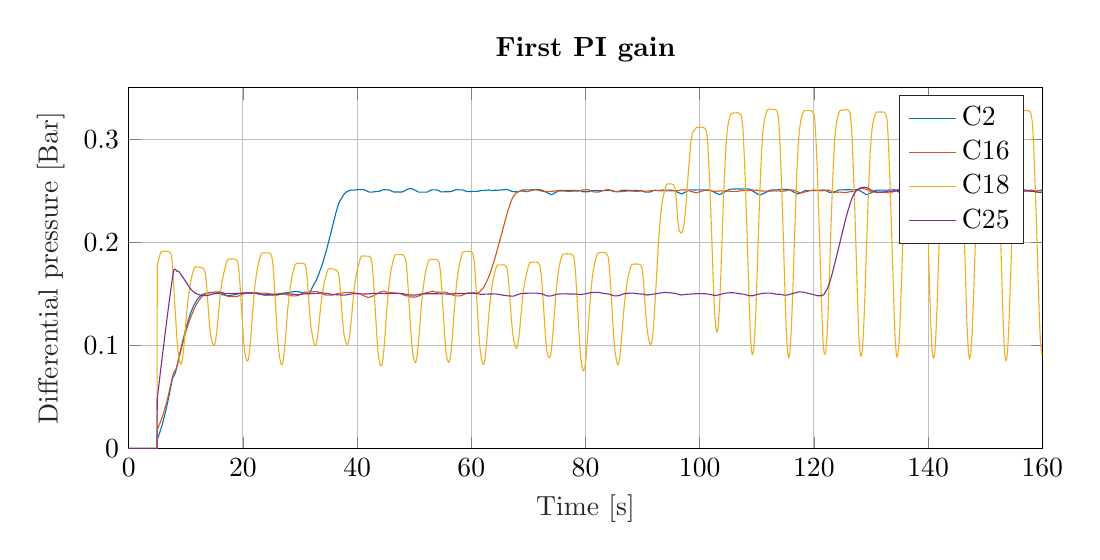
\begin{tikzpicture}

\begin{axis}[%
width=4.568in,
height=1.803in,
at={(0.766in,0.486in)},
scale only axis,
xmin=0,
xmax=160,
xlabel style={font=\color{white!15!black}},
xlabel={Time [s]},
ymin=0,
ymax=0.35,
ylabel style={font=\color{white!15!black}},
ylabel={Differential pressure [Bar]},
axis background/.style={fill=white},
title style={font=\bfseries},
title={First PI gain},
xmajorgrids,
ymajorgrids,
legend style={legend cell align=left, align=left, draw=white!15!black}
]
\addplot [color=mycolor1]
  table[row sep=crcr]{%
0	0\\
4.94999999999999	0\\
5	0.00897482893449819\\
5.15000000000001	0.0110153958944181\\
5.40000000000001	0.0148765884652846\\
5.75	0.020821114369511\\
5.84999999999999	0.0226539589442893\\
6.19999999999999	0.0300464320625622\\
6.34999999999999	0.0333760997067429\\
6.5	0.0368707233626537\\
6.84999999999999	0.0454667644183644\\
7.05000000000001	0.0507025904203431\\
7.34999999999999	0.0589870478983414\\
7.65000000000001	0.0673448191593309\\
7.69999999999999	0.0683223362658794\\
8.05000000000001	0.0719452590420246\\
8.09999999999999	0.0725256598240378\\
8.15000000000001	0.0733015640273607\\
8.30000000000001	0.0761608015640149\\
8.34999999999999	0.0772299608993023\\
8.55000000000001	0.0821664222874006\\
8.90000000000001	0.0908296676441864\\
9.09999999999999	0.0957783479960881\\
9.44999999999999	0.104062805474086\\
9.94999999999999	0.115090420332365\\
10.15	0.119189882697952\\
10.4	0.123863636363637\\
10.65	0.128299120234601\\
10.85	0.131561583577707\\
11.25	0.137035679374378\\
11.5	0.13977883675463\\
11.85	0.143310117302065\\
12.05	0.145002443792777\\
12.25	0.146383186705776\\
12.6	0.148350439882705\\
12.85	0.149309628543506\\
13.15	0.150000000000006\\
13.45	0.150433773216037\\
13.65	0.150592619745851\\
13.95	0.150922531769311\\
14.3	0.151105816226789\\
14.7	0.151093597262957\\
14.95	0.151050830889545\\
15.25	0.151075268817209\\
15.55	0.15078812316716\\
16	0.150018328445753\\
16.45	0.149260752688178\\
17.2	0.148234359726303\\
17.75	0.148466520039108\\
18.8	0.149627321603134\\
19.55	0.150439882697952\\
19.7	0.150708699902253\\
20.25	0.150769794721413\\
20.45	0.15098362658847\\
21.2	0.151246334310855\\
22.45	0.15081867057674\\
24.1	0.148930840664718\\
24.95	0.148936950146634\\
25.3	0.149028592375373\\
25.5	0.149120234604112\\
26	0.14979838709678\\
26.35	0.150152737047904\\
26.55	0.150250488758559\\
27	0.150794232649076\\
27.3	0.150891984359731\\
27.5	0.150995845552302\\
27.75	0.1511485826002\\
28.3	0.151600684261979\\
28.55	0.151906158357775\\
29.2	0.152492668621704\\
29.9	0.151930596285439\\
30.2	0.151594574780063\\
30.45	0.151325757575762\\
30.75	0.151032502443798\\
31.1	0.150598729227767\\
31.25	0.150769794721413\\
31.65	0.151771749755625\\
31.75	0.152315493646142\\
31.9	0.153274682306943\\
31.95	0.153757331378301\\
32.2	0.156860948191593\\
32.8	0.16270161290322\\
32.95	0.164595552297158\\
33.1	0.166544477028339\\
33.65	0.174816715542534\\
33.75	0.176282991202356\\
34.15	0.183241691104598\\
34.65	0.192906891495596\\
34.95	0.199340175953068\\
35.5	0.2113086510264\\
35.65	0.214589442815253\\
36.15	0.225800342130981\\
36.25	0.227920332355808\\
36.55	0.233748778103632\\
36.7	0.236430840664724\\
36.9	0.239473362658856\\
36.95	0.24002321603129\\
37.2	0.24206378299121\\
37.6	0.245839442815253\\
37.75	0.246981915933532\\
37.85	0.247635630498536\\
38.1	0.24881476050831\\
38.4	0.249761730205279\\
38.85	0.2506903714565\\
39	0.250843108504398\\
39.5	0.250727028347995\\
39.85	0.251160801564026\\
40.2	0.251295210166177\\
41.2	0.251179130009774\\
41.4	0.250739247311827\\
41.75	0.249847262952102\\
41.95	0.249181329423266\\
42.2	0.248771994134898\\
42.65	0.248881964809385\\
43.75	0.249566226783969\\
44	0.249761730205279\\
44.6	0.251228005865102\\
44.75	0.251228005865102\\
45.65	0.250800342130987\\
45.8	0.250574291300097\\
46.1	0.249566226783969\\
46.35	0.249040811339199\\
46.6	0.248894183773217\\
47.9	0.24897971652004\\
48.2	0.249731182795699\\
48.85	0.251588465298141\\
49.05	0.251997800586508\\
49.6	0.252138318670575\\
49.7	0.251967253176929\\
50.05	0.250946969696969\\
50.25	0.250378787878788\\
50.45	0.249792277614858\\
50.7	0.249046920821115\\
50.8	0.248826979472142\\
51.15	0.248826979472142\\
51.35	0.248808651026394\\
51.9	0.248820869990226\\
52.25	0.248863636363637\\
52.35	0.249046920821115\\
52.8	0.250610948191593\\
52.9	0.250800342130987\\
53.2	0.251008064516128\\
53.65	0.25102028347996\\
53.9	0.250928641251221\\
54.2	0.250549853372434\\
54.45	0.249773949169111\\
54.65	0.249138563049854\\
54.95	0.249004154447704\\
55.25	0.249132453567938\\
55.4	0.249126344086022\\
55.9	0.249248533724341\\
56.05	0.249199657869013\\
56.55	0.249480694037146\\
56.95	0.250439882697947\\
57.3	0.251301319648093\\
57.5	0.25121578690127\\
57.8	0.251008064516128\\
58.2	0.250940860215053\\
58.5	0.25102028347996\\
59.2	0.2493096285435\\
61.2	0.249633431085044\\
61.45	0.250054985337243\\
61.7	0.250421554252199\\
62.15	0.250476539589442\\
62.8	0.250751466275659\\
63.15	0.250873655913978\\
63.25	0.250873655913978\\
63.55	0.250238269794721\\
63.75	0.250293255131965\\
64	0.250531524926686\\
64.15	0.250653714565004\\
64.55	0.250623167155425\\
64.85	0.250775904203323\\
66.25	0.251368523949168\\
66.4	0.251203567937438\\
67.1	0.249535679374389\\
67.4	0.249217986314761\\
68.3	0.249169110459434\\
68.65	0.25019550342131\\
68.95	0.250904203323557\\
69.3	0.250898093841641\\
69.95	0.25102028347996\\
70.45	0.251075268817203\\
70.7	0.251179130009774\\
71	0.251166911045942\\
72.05	0.251203567937438\\
72.4	0.250684261974584\\
73.45	0.247867790811341\\
73.9	0.246529814271753\\
74	0.246505376344089\\
74.15	0.246590909090912\\
74.75	0.248387096774195\\
75.1	0.249456256109482\\
75.45	0.250488758553274\\
75.6	0.250537634408602\\
76	0.250513196480938\\
78.5	0.25032991202346\\
78.95	0.250323802541544\\
79.15	0.250219941348973\\
79.4	0.249431818181819\\
79.65	0.249163000977518\\
80.15	0.249217986314761\\
80.5	0.249199657869013\\
80.75	0.249755620723363\\
80.95	0.250122189638319\\
81.2	0.250085532746823\\
82	0.250250488758553\\
82.75	0.250323802541573\\
83.4	0.250274926686245\\
83.9	0.250494868035219\\
84.6	0.250164956011787\\
84.8	0.249541788856362\\
85.1	0.249266862170145\\
85.5	0.249382942326548\\
85.85	0.249505131964867\\
85.95	0.249657869012765\\
86.2	0.250366568915013\\
86.5	0.250604838709734\\
86.65	0.25054985337249\\
86.9	0.250635386119313\\
87.75	0.250537634408659\\
88.05	0.250507086999079\\
88.65	0.250342130987349\\
89.1	0.250354349951181\\
89.8	0.250274926686274\\
90.15	0.249486803519119\\
90.3	0.249053030303088\\
90.55	0.248753665689208\\
91.35	0.248906402737106\\
91.65	0.24972507331384\\
91.9	0.250354349951181\\
92.1	0.25061094819165\\
92.45	0.250476539589499\\
92.9	0.250574291300154\\
93.1	0.250653714565061\\
93.65	0.250867546432119\\
95.45	0.250531524926743\\
95.6	0.250146627566039\\
96.05	0.248924731182854\\
96.6	0.247537878787938\\
96.85	0.247201857282562\\
97.15	0.247800586510323\\
97.35	0.248429863147663\\
98.05	0.250452101661836\\
98.3	0.250916422287446\\
98.45	0.251050830889596\\
99.05	0.250885874877866\\
100.2	0.251014173998101\\
100.85	0.250995845552353\\
101	0.250983626588521\\
101.5	0.250977517106605\\
101.8	0.250891984359782\\
102	0.250311583577769\\
102.35	0.249321847507389\\
102.65	0.248472629521075\\
103.4	0.246493157380314\\
103.5	0.246584799609053\\
103.65	0.246853616813354\\
104	0.247947214076305\\
104.75	0.25008553274688\\
105.2	0.251496823069459\\
105.3	0.251667888563105\\
105.5	0.251777859237592\\
105.7	0.25176564027376\\
106.05	0.251893939393995\\
106.35	0.251881720430163\\
106.6	0.251955034213154\\
106.95	0.25176564027376\\
107.3	0.251887829912079\\
107.75	0.251906158357826\\
108.45	0.252046676441893\\
108.7	0.251606793743946\\
109	0.250702590420389\\
109.15	0.250244379276694\\
110.3	0.246505376344146\\
110.6	0.246242668621761\\
110.7	0.246254887585593\\
111.05	0.247146871945318\\
111.2	0.247623411534761\\
111.5	0.248350439882756\\
111.65	0.248765884653039\\
112.1	0.25025048875861\\
112.35	0.250812561094875\\
112.55	0.250824780058707\\
112.75	0.250830889540623\\
113.05	0.25087976539595\\
113.3	0.25087976539595\\
113.6	0.251014173998101\\
114.15	0.251209677419411\\
114.5	0.251331867057729\\
114.75	0.251356304985393\\
115	0.251411290322636\\
115.55	0.251423509286468\\
115.7	0.251319648093897\\
116.05	0.250213831867114\\
116.25	0.249492913001035\\
117	0.24732404692088\\
117.1	0.247232404692141\\
117.35	0.24735459433046\\
117.6	0.247977761485885\\
118.45	0.250152737047955\\
118.75	0.250293255132021\\
119.05	0.250256598240526\\
119.35	0.250256598240526\\
119.55	0.250238269794778\\
119.75	0.250262707722442\\
120	0.250323802541601\\
120.8	0.250543743890574\\
121.6	0.250916422287446\\
121.85	0.25077590420338\\
122.25	0.249926686217066\\
122.55	0.248943059628601\\
122.75	0.248558162267898\\
123.15	0.24837487781042\\
123.4	0.248435972629579\\
123.6	0.248741446725376\\
123.85	0.249419599218044\\
124.3	0.250806451612959\\
124.6	0.251032502443849\\
125.2	0.251069159335344\\
125.5	0.251063049853428\\
126.2	0.251179130009831\\
126.4	0.251154692082167\\
126.75	0.251008064516185\\
127.7	0.251111925708756\\
128.15	0.249841153470243\\
128.55	0.248552052785982\\
128.8	0.247708944281584\\
129.1	0.246578690127137\\
129.3	0.246389296187743\\
129.65	0.247140762463403\\
130.35	0.249150782013743\\
130.9	0.250696480938473\\
131.1	0.250818670576791\\
131.35	0.250678152492725\\
131.65	0.250696480938473\\
133	0.250812561094875\\
134.1	0.251160801564083\\
134.4	0.25044599217992\\
134.95	0.248692570870048\\
135.15	0.248191593352942\\
135.45	0.248093841642287\\
135.7	0.248002199413548\\
135.95	0.248008308895464\\
136.1	0.24824046920827\\
136.4	0.249138563049911\\
137	0.250702590420389\\
137.3	0.25054985337249\\
137.5	0.250568181818238\\
137.85	0.250397116324592\\
138.4	0.250183284457535\\
139.6	0.250152737047955\\
139.95	0.250274926686274\\
140.2	0.250177174975619\\
140.4	0.249835043988327\\
141.65	0.249859481915991\\
142.5	0.24956011730211\\
143.1	0.249731182795756\\
143.55	0.249688416422345\\
145.2	0.249987781036225\\
145.45	0.250354349951181\\
146.85	0.25041544477034\\
147	0.250171065493703\\
147.5	0.250177174975619\\
148	0.250061094819216\\
148.8	0.249602883675522\\
149.5	0.249639540567017\\
149.85	0.250659824046977\\
150	0.251063049853428\\
150.25	0.251564027370534\\
150.45	0.251637341153526\\
151.1	0.251777859237592\\
151.35	0.251148582600251\\
151.5	0.250629276637397\\
151.8	0.249957233626645\\
151.95	0.249902248289402\\
152.55	0.250317693059685\\
152.7	0.250458211143751\\
153.05	0.250494868035247\\
153.95	0.250812561094875\\
154.45	0.250684261974641\\
154.55	0.250476539589499\\
155.3	0.248032746823128\\
155.4	0.247818914956071\\
156.15	0.247739491691163\\
156.4	0.248448191593411\\
156.55	0.248839198436031\\
157	0.249853372434075\\
157.25	0.249816715542579\\
157.95	0.249749511241504\\
158.3	0.249853372434075\\
158.6	0.249865591397906\\
159	0.249938905180898\\
159.5	0.250109970674544\\
159.8	0.250164956011787\\
160.2	0.250012218963889\\
};
\addlegendentry{C2}

\addplot [color=mycolor2]
  table[row sep=crcr]{%
0	0\\
4.94999999999999	0\\
5	0.0187683284457592\\
5.15000000000001	0.0204239980449756\\
5.44999999999999	0.0243585043988332\\
5.84999999999999	0.0299547898338233\\
6.15000000000001	0.0352700391006806\\
6.40000000000001	0.0400354349951044\\
6.55000000000001	0.0430840664711525\\
6.94999999999999	0.051893939393949\\
7.09999999999999	0.0555229716520103\\
7.30000000000001	0.0605083088954075\\
7.65000000000001	0.0692754154447641\\
7.80000000000001	0.0722812805474007\\
7.84999999999999	0.0730083088953961\\
8	0.0744684750733029\\
8.09999999999999	0.0754582111436832\\
8.30000000000001	0.0772849462365457\\
8.34999999999999	0.0780364125122048\\
8.84999999999999	0.088575268817209\\
9.30000000000001	0.0985703812316672\\
9.44999999999999	0.101625122189631\\
9.69999999999999	0.107025904203311\\
10	0.112927663734126\\
10.2	0.116520039100692\\
10.45	0.120766129032262\\
10.75	0.125653714565004\\
10.85	0.127211632453566\\
11.1	0.130529081133915\\
11.5	0.135856549364604\\
11.75	0.138636363636351\\
12.1	0.141984359726308\\
12.3	0.143682795698936\\
12.7	0.146535923753675\\
13	0.14831378299121\\
13.2	0.149266862170094\\
13.4	0.149926686217015\\
14.1	0.151417399804501\\
15	0.151728983382213\\
15.25	0.151948924731187\\
15.9	0.151832844574784\\
16.15	0.151484604105576\\
16.8	0.149554007820143\\
17.3	0.147947214076254\\
17.55	0.147525659824055\\
17.8	0.147556207233634\\
18.95	0.147543988269803\\
19.2	0.147928885630506\\
19.6	0.148814760508316\\
19.95	0.149688416422293\\
20.5	0.150727028348001\\
21	0.150727028348001\\
21.7	0.15078812316716\\
22.05	0.150824780058656\\
22.25	0.150940860215059\\
22.4	0.1511485826002\\
22.6	0.151173020527864\\
22.85	0.150739247311833\\
23.45	0.150782013685244\\
23.75	0.150739247311833\\
24.6	0.150452101661784\\
24.8	0.150030547409585\\
25.05	0.14943792766374\\
25.35	0.148710899315745\\
25.6	0.148637585532754\\
26.15	0.148863636363643\\
26.4	0.149511241446731\\
26.8	0.150134408602156\\
27.15	0.150097751710661\\
27.55	0.149444037145656\\
27.75	0.149156891495608\\
27.85	0.148985826001962\\
28.05	0.148527614858267\\
28.2	0.148356549364621\\
28.75	0.14814882697948\\
29.4	0.148179374389059\\
29.6	0.148423753665696\\
29.75	0.148735337243409\\
30	0.149486803519068\\
30.3	0.150177174975568\\
30.85	0.151564027370483\\
31.1	0.151832844574784\\
31.35	0.151625122189643\\
31.8	0.151777859237541\\
32.1	0.152010019550346\\
32.3	0.152181085043992\\
32.85	0.152242179863151\\
32.95	0.152284946236563\\
33.15	0.152010019550346\\
33.3	0.151686217008802\\
33.55	0.151197458455528\\
33.9	0.150268817204307\\
34.2	0.149425708699908\\
34.6	0.148869745845559\\
34.8	0.148863636363643\\
34.95	0.148790322580652\\
35.15	0.148881964809391\\
35.3	0.148881964809391\\
35.65	0.148991935483878\\
35.85	0.149175219941355\\
36.35	0.149981671554258\\
36.7	0.150238269794727\\
37.1	0.150782013685244\\
37.55	0.151001955034218\\
37.8	0.151289100684266\\
38.2	0.151319648093846\\
39.35	0.15150904203324\\
39.6	0.150977517106554\\
39.8	0.150562072336271\\
40	0.150452101661784\\
40.35	0.150384897360709\\
40.55	0.150006109481922\\
40.9	0.148900293255139\\
41.7	0.146975806451621\\
41.95	0.146584799609002\\
42.15	0.146706989247321\\
42.45	0.147324046920829\\
42.7	0.147898338220926\\
42.9	0.148411534701864\\
44	0.15164345063539\\
44.6	0.152743157380257\\
44.8	0.152651515151518\\
44.9	0.15249877810362\\
45.15	0.151893939393943\\
45.4	0.151282991202351\\
45.55	0.151160801564032\\
45.8	0.151282991202351\\
46.3	0.151075268817209\\
46.55	0.151026392961882\\
46.8	0.15081867057674\\
46.95	0.150751466275665\\
47.15	0.150586510263935\\
47.6	0.150189393939399\\
47.8	0.149841153470192\\
48.3	0.148539833822099\\
48.95	0.147886119257095\\
49.45	0.146969696969705\\
49.55	0.146957478005874\\
49.8	0.147061339198444\\
50.15	0.146945259042042\\
50.3	0.147030791788865\\
50.7	0.147739491691112\\
51.65	0.150177174975568\\
51.85	0.150690371456506\\
52.25	0.151392961876837\\
52.75	0.151875610948196\\
53.25	0.152675953079182\\
53.4	0.152504887585536\\
53.75	0.151722873900297\\
53.85	0.151600684261979\\
54.25	0.151661779081138\\
54.55	0.151722873900297\\
54.85	0.151698435972634\\
55.35	0.1518389540567\\
55.75	0.15134408602151\\
56.15	0.150250488758559\\
56.85	0.148655913978502\\
57.3	0.148173264907143\\
57.7	0.148112170087984\\
57.85	0.148112170087984\\
58.1	0.148167155425227\\
58.3	0.148490957966771\\
58.6	0.14927297165201\\
59.3	0.150873655913983\\
59.5	0.150959188660806\\
59.85	0.150885874877815\\
60.1	0.150922531769311\\
60.95	0.150922531769311\\
61.25	0.151264662756603\\
61.5	0.152223851417403\\
61.7	0.153421309872925\\
61.85	0.154294965786903\\
61.95	0.154838709677421\\
62.3	0.157691837732159\\
62.4	0.158730449657867\\
62.9	0.164534457477998\\
63.15	0.168108504398816\\
63.4	0.171994134897375\\
63.6	0.175305474095808\\
64.05	0.18311950146628\\
64.4	0.189876588465296\\
64.85	0.19902248289344\\
65.9	0.220417888563048\\
66.25	0.227779814271742\\
66.5	0.232245845552285\\
66.95	0.239565004887567\\
67.2	0.242925219941355\\
67.35	0.24437316715543\\
67.5	0.245515640273709\\
67.8	0.247519550342133\\
67.95	0.248295454545456\\
68.2	0.249163000977518\\
68.55	0.249816715542522\\
69.1	0.249688416422288\\
69.45	0.249346285434996\\
69.95	0.249401270772239\\
70.1	0.249663978494624\\
70.85	0.250922531769305\\
71.2	0.251032502443792\\
71.7	0.250806451612902\\
72.45	0.249468475073314\\
73.65	0.249272971652005\\
74	0.249492913000978\\
74.15	0.249480694037146\\
74.85	0.250152737047898\\
75.1	0.250109970674487\\
75.35	0.249963343108504\\
76.8	0.249657869012708\\
77.1	0.249535679374389\\
77.35	0.249651759530792\\
77.75	0.249725073313783\\
78.15	0.249786168132943\\
78.3	0.24980449657869\\
78.5	0.249706744868035\\
78.8	0.24986559139785\\
78.9	0.249847262952102\\
79.45	0.250830889540566\\
79.75	0.250904203323557\\
80.25	0.251240224828933\\
80.5	0.25105083088954\\
80.7	0.250543743890518\\
80.9	0.250103861192571\\
81.1	0.249657869012708\\
81.6	0.248833088954058\\
81.7	0.248808651026394\\
81.95	0.248936950146629\\
82.3	0.248900293255133\\
82.45	0.249095796676443\\
82.85	0.249896138807429\\
83.2	0.250366568914956\\
83.35	0.250610948191593\\
83.55	0.251001955034212\\
83.95	0.251331867057672\\
84.6	0.250513196480938\\
85.25	0.249444037145651\\
85.6	0.249101906158359\\
86	0.249315738025416\\
86.2	0.249334066471164\\
86.65	0.249291300097752\\
86.9	0.249389051808407\\
87.2	0.249847262952102\\
87.4	0.250006109481916\\
87.75	0.249847262952102\\
88.1	0.249761730205279\\
88.25	0.249761730205279\\
88.45	0.249706744868035\\
89.15	0.249560117302053\\
89.5	0.24980449657869\\
89.7	0.249890029325513\\
89.9	0.249749511241447\\
90.35	0.249602883675465\\
90.6	0.249761730205279\\
90.7	0.249731182795699\\
90.95	0.249883919843597\\
91.35	0.249914467253177\\
91.65	0.250256598240469\\
91.9	0.250482649071358\\
92.25	0.250452101661779\\
92.85	0.250103861192571\\
93.2	0.250116080156403\\
93.4	0.249981671554252\\
94.25	0.250073313782991\\
94.9	0.249957233626617\\
95.5	0.250054985337272\\
96.05	0.250122189638347\\
96.65	0.250855327468287\\
97.05	0.250782013685296\\
97.4	0.25110581622684\\
97.7	0.250995845552353\\
97.85	0.250782013685296\\
98.1	0.25028103616819\\
99.05	0.248625366568973\\
99.5	0.248338220918924\\
99.65	0.248484848484907\\
99.9	0.248979716520097\\
100.1	0.249291300097809\\
100.45	0.249822825024495\\
100.65	0.250128299120291\\
100.8	0.250372678396928\\
101.45	0.250733137829968\\
102.05	0.250195503421367\\
102.3	0.249773949169168\\
102.45	0.249639540567017\\
102.8	0.249663978494681\\
103.1	0.249804496578747\\
103.7	0.250018328445805\\
104.25	0.249810606060663\\
104.45	0.250122189638375\\
104.8	0.249865591397906\\
105.05	0.249737292277672\\
105.75	0.249492913001035\\
106.35	0.24952956989253\\
106.6	0.24952956989253\\
107	0.249896138807486\\
107.7	0.250507086999079\\
108.15	0.250348240469265\\
108.7	0.250342130987349\\
108.95	0.250769794721464\\
109.1	0.250983626588521\\
109.3	0.250818670576791\\
109.5	0.250678152492725\\
109.85	0.250653714565061\\
110.2	0.250464320625667\\
110.9	0.249877810361738\\
112.15	0.249682306940429\\
112.3	0.249743401759588\\
112.7	0.249786168132999\\
113	0.249987781036225\\
113.25	0.249957233626645\\
113.5	0.249951124144729\\
113.65	0.2500549853373\\
113.85	0.249963343108561\\
114.2	0.249572336265942\\
114.6	0.249700635386176\\
114.9	0.249914467253234\\
115.05	0.249993890518141\\
115.45	0.250763685239548\\
115.95	0.251014173998101\\
116.15	0.250904203323614\\
116.55	0.250439882698004\\
117.15	0.24906524926692\\
117.45	0.248399315738084\\
117.6	0.248173264907194\\
117.8	0.248112170088035\\
119.5	0.250482649071415\\
119.7	0.250604838709734\\
120.15	0.250690371456557\\
120.5	0.250476539589499\\
120.7	0.250568181818238\\
120.85	0.250409335288424\\
121	0.250164956011787\\
121.25	0.250061094819216\\
121.45	0.249969452590477\\
121.85	0.250500977517163\\
122.15	0.250690371456557\\
122.6	0.250678152492725\\
122.9	0.250116080156459\\
123.1	0.249602883675522\\
123.65	0.249071358748836\\
124	0.248729227761544\\
124.65	0.248771994134955\\
125.4	0.248552052785982\\
125.6	0.248478739002991\\
125.9	0.248741446725376\\
126.1	0.248985826002013\\
126.55	0.249413489736128\\
126.7	0.249389051808464\\
127	0.249798387096831\\
127.25	0.250109970674544\\
127.5	0.250543743890574\\
127.75	0.251142473118335\\
128.2	0.25242546432068\\
128.4	0.252443792766428\\
129	0.251814516129087\\
129.15	0.251484604105627\\
130.25	0.248741446725376\\
130.65	0.248765884653039\\
130.9	0.248698680351964\\
131.1	0.248741446725376\\
131.4	0.248729227761544\\
131.75	0.248600928641309\\
132.2	0.248643695014721\\
132.4	0.248643695014721\\
132.6	0.248515395894486\\
133.1	0.248020527859296\\
133.2	0.248063294232708\\
134.15	0.249663978494681\\
134.45	0.250684261974641\\
134.6	0.25107526881726\\
135.25	0.252303274682362\\
135.5	0.252284946236614\\
135.95	0.251417399804552\\
136.35	0.250409335288424\\
136.55	0.250012218963889\\
136.9	0.249749511241504\\
137.2	0.249780058651083\\
137.35	0.249792277614915\\
137.7	0.249963343108561\\
138.05	0.249877810361738\\
138.55	0.249621212121269\\
138.9	0.249651759530849\\
139.15	0.249480694037203\\
139.35	0.249144672531827\\
139.6	0.249083577712668\\
139.95	0.24923020527865\\
140.15	0.249248533724398\\
140.55	0.24939516129038\\
140.75	0.250103861192628\\
140.85	0.250391006842676\\
141.65	0.252028347996145\\
141.8	0.252010019550397\\
142	0.251625122189694\\
142.3	0.250995845552353\\
142.6	0.250189393939451\\
142.9	0.249517350928699\\
143.3	0.249236314760566\\
145.3	0.249138563049911\\
145.5	0.2490957966765\\
145.6	0.249004154447761\\
145.8	0.248649804496637\\
146.75	0.248875855327526\\
146.95	0.249468475073371\\
147.55	0.251026392961933\\
147.75	0.251454056696048\\
147.9	0.251716764418433\\
148.15	0.251771749755676\\
148.7	0.250977517106605\\
149.4	0.250048875855384\\
149.75	0.249926686217066\\
150.1	0.249596774193606\\
151.15	0.249468475073371\\
151.55	0.249291300097809\\
151.9	0.24903470185734\\
152.2	0.248643695014721\\
152.45	0.248643695014721\\
152.75	0.248576490713646\\
152.95	0.248417644183831\\
153.2	0.248637585532805\\
153.55	0.249346285435053\\
153.75	0.249523460410614\\
154.2	0.249798387096831\\
154.5	0.249676197458513\\
155.55	0.248521505376402\\
155.8	0.24834433040084\\
155.95	0.248497067448739\\
156.4	0.249138563049911\\
156.6	0.249462365591455\\
156.85	0.249743401759588\\
157.95	0.250830889540623\\
158.15	0.250763685239548\\
158.75	0.250061094819216\\
159.25	0.250128299120291\\
159.5	0.25038489736076\\
159.75	0.250818670576791\\
159.95	0.251087487781092\\
160.2	0.251093597263008\\
};
\addlegendentry{C16}

\addplot [color=mycolor3]
  table[row sep=crcr]{%
0	0\\
4.94999999999999	0\\
5	0.177584310850449\\
5.19999999999999	0.182209188660806\\
5.30000000000001	0.184524682306943\\
5.40000000000001	0.186485826001956\\
5.55000000000001	0.189290078201367\\
5.59999999999999	0.189907135874876\\
5.80000000000001	0.191232893450632\\
5.90000000000001	0.191275659824043\\
6.09999999999999	0.191226783968716\\
6.34999999999999	0.191391739980446\\
6.55000000000001	0.191397849462362\\
6.90000000000001	0.191232893450632\\
7.09999999999999	0.190829667644181\\
7.19999999999999	0.190328690127075\\
7.34999999999999	0.18937561094819\\
7.40000000000001	0.188446969696969\\
7.55000000000001	0.183925953079182\\
7.59999999999999	0.181323313782997\\
7.65000000000001	0.177474340175962\\
7.80000000000001	0.165518084066463\\
7.84999999999999	0.161088709677415\\
8	0.146597018572834\\
8.05000000000001	0.141868279569906\\
8.09999999999999	0.137432795698913\\
8.25	0.124651759530792\\
8.34999999999999	0.115065982404701\\
8.5	0.102688172043003\\
8.55000000000001	0.0989002932551273\\
8.59999999999999	0.0962487781036145\\
8.75	0.0907074780058679\\
8.80000000000001	0.0890456989247355\\
8.94999999999999	0.0844819159335373\\
9	0.0833699902248384\\
9.09999999999999	0.0823497067448784\\
9.15000000000001	0.0819159335288475\\
9.19999999999999	0.0819403714565112\\
9.25	0.0827956989247411\\
9.40000000000001	0.0864674975562139\\
9.44999999999999	0.0881781524926737\\
9.55000000000001	0.0930107526881727\\
9.65000000000001	0.0980021994134859\\
9.69999999999999	0.100928641251215\\
9.84999999999999	0.110771016617804\\
9.94999999999999	0.117992424242431\\
10.15	0.131378299120229\\
10.2	0.134390273704781\\
10.35	0.142320381231684\\
10.4	0.144678641251232\\
10.55	0.150470430107532\\
10.6	0.152718719452594\\
10.65	0.154789833822093\\
10.75	0.158027859237535\\
10.85	0.161430840664707\\
11.05	0.166739980449648\\
11.15	0.168976050830878\\
11.3	0.172177419354853\\
11.35	0.173093841642242\\
11.5	0.175409335288379\\
11.55	0.175867546432073\\
11.8	0.176466275659834\\
12.15	0.176099706744878\\
12.5	0.17578201368525\\
12.75	0.175519305962865\\
13	0.174975562072348\\
13.05	0.174847262952113\\
13.1	0.174523460410569\\
13.3	0.172605083088968\\
13.35	0.171462609970689\\
13.55	0.164228983382202\\
13.6	0.161253665689145\\
13.8	0.146126588465307\\
13.85	0.142185972629534\\
14	0.130742913000972\\
14.05	0.126783968719451\\
14.1	0.123271016617792\\
14.2	0.117369257087006\\
14.25	0.114112903225816\\
14.3	0.111681329423277\\
14.45	0.107716275659811\\
14.5	0.106219452590409\\
14.55	0.104905913978484\\
14.7	0.102022238514166\\
14.75	0.101435728250237\\
14.9	0.100183284457472\\
14.95	0.100048875855322\\
15	0.100537634408596\\
15.15	0.103103616813286\\
15.2	0.104435483870958\\
15.35	0.110092864125136\\
15.4	0.112438905180852\\
15.5	0.117803030303037\\
15.6	0.123051075268819\\
15.7	0.129325513196477\\
15.8	0.135031769305954\\
15.9	0.141275659824061\\
16.1	0.152181085043992\\
16.15	0.154533235581624\\
16.35	0.162005131964804\\
16.4	0.163514173998038\\
16.5	0.165854105571839\\
16.6	0.168841642228728\\
16.8	0.173301564027383\\
17	0.177926441837741\\
17.1	0.179814271749763\\
17.25	0.182478005865107\\
17.3	0.18305840664712\\
17.45	0.183712121212125\\
17.6	0.183822091886611\\
18.2	0.183919843597266\\
18.5	0.183803763440864\\
18.65	0.183498289345067\\
18.85	0.182783479960904\\
19.05	0.181347751710661\\
19.1	0.180370234604112\\
19.25	0.175708699902259\\
19.3	0.173026637341167\\
19.5	0.15815615835777\\
19.55	0.154123900293257\\
19.75	0.136968475073303\\
19.8	0.132490224828928\\
19.95	0.119464809384169\\
20	0.114784946236568\\
20.05	0.110471652003923\\
20.2	0.0995784457477953\\
20.25	0.096212121212119\\
20.3	0.0939516129032256\\
20.45	0.0893817204301115\\
20.5	0.088239247311833\\
20.65	0.0855755131964884\\
20.7	0.0850012218963911\\
20.75	0.0849217986314841\\
20.85	0.0850806451612982\\
20.9	0.0855632942326565\\
20.95	0.0868157380254218\\
21.1	0.091715542521996\\
21.15	0.0938660801564026\\
21.2	0.0966642228738976\\
21.3	0.102535434995104\\
21.35	0.105645161290312\\
21.4	0.109127565982419\\
21.55	0.120112414467258\\
21.65	0.128189149560114\\
21.85	0.142870234604118\\
21.9	0.146181573802551\\
22.1	0.157416911045942\\
22.25	0.163636363636357\\
22.3	0.166037390029317\\
22.35	0.168236803519051\\
22.45	0.171676441837747\\
22.5	0.173509286412525\\
22.55	0.175073313783003\\
22.9	0.183333333333337\\
22.95	0.184457478005868\\
23	0.185441104594332\\
23.15	0.18786045943304\\
23.2	0.188648582600194\\
23.25	0.189149560117301\\
23.5	0.189876588465296\\
24.6	0.189894916911044\\
24.8	0.189235092864124\\
25	0.187744379276637\\
25.05	0.186650782013686\\
25.2	0.181158357771267\\
25.25	0.17887341153471\\
25.3	0.175464320625622\\
25.45	0.163159824046915\\
25.5	0.158809872922774\\
25.65	0.14525293255133\\
25.8	0.131671554252193\\
25.9	0.122617302052788\\
25.95	0.117748044965793\\
26	0.113294232649082\\
26.2	0.098417644183769\\
26.25	0.095442326490712\\
26.35	0.0914528347996111\\
26.4	0.0896077712610008\\
26.5	0.0866080156402802\\
26.6	0.08374266862171\\
26.65	0.0826612903225907\\
26.7	0.0821419843597369\\
26.85	0.081115591397861\\
26.9	0.0815249266862281\\
27.05	0.085263929618776\\
27.1	0.0870601173020589\\
27.15	0.0894855816226823\\
27.3	0.0971224340175922\\
27.35	0.100177174975556\\
27.45	0.107038123167143\\
27.5	0.11041666666668\\
27.6	0.117943548387103\\
27.8	0.131873167155419\\
27.85	0.134958455522963\\
27.95	0.140261485826016\\
28	0.143059628543512\\
28.05	0.145662267839697\\
28.15	0.149957233626594\\
28.2	0.15203445747801\\
28.25	0.154398826979474\\
28.3	0.15661045943304\\
28.55	0.165426441837724\\
28.75	0.170558406647103\\
29	0.176020283479971\\
29.15	0.178305229716528\\
29.2	0.178800097751719\\
29.4	0.179453812316723\\
29.55	0.179582111436957\\
30.3	0.179930351906165\\
30.6	0.179692082111444\\
30.75	0.179191104594338\\
30.95	0.177682062561104\\
31	0.176509042033246\\
31.2	0.1687927663734\\
31.25	0.165866324535671\\
31.35	0.158247800586508\\
31.45	0.150586510263935\\
31.55	0.142864125122202\\
31.65	0.135227272727263\\
31.7	0.131219452590415\\
31.75	0.127755376344084\\
31.85	0.12226906158358\\
31.9	0.11923875855328\\
31.95	0.116593352883683\\
32	0.114876588465307\\
32.1	0.11190127077225\\
32.25	0.10717864125121\\
32.35	0.104239980449648\\
32.4	0.102950879765388\\
32.5	0.101099706744861\\
32.55	0.100250488758547\\
32.6	0.0996945259041979\\
32.65	0.0997678396871891\\
32.8	0.101038611925702\\
32.85	0.10191226783968\\
32.95	0.104863147605073\\
33	0.106384408602139\\
33.05	0.108260019550329\\
33.25	0.117302052785931\\
33.3	0.120039100684266\\
33.35	0.122934995112416\\
33.65	0.138666911045931\\
33.75	0.143780547409591\\
33.8	0.146034946236568\\
33.95	0.151460166177912\\
34	0.153476295210169\\
34.05	0.155217497556208\\
34.15	0.157740713587486\\
34.25	0.160813782991198\\
34.5	0.166697214076237\\
34.7	0.170796676441825\\
34.9	0.173845307917901\\
34.95	0.1742668621701\\
35.3	0.174651759530803\\
35.7	0.174364613880755\\
36.15	0.173594819159348\\
36.3	0.173399315738038\\
36.5	0.172470674486817\\
36.7	0.17074169110461\\
36.75	0.169605327468219\\
36.9	0.164119012707715\\
36.95	0.161565249266857\\
37	0.158082844574778\\
37.15	0.146957478005874\\
37.25	0.139332844574767\\
37.4	0.128250244379274\\
37.45	0.12486559139785\\
37.6	0.116184017595316\\
37.65	0.11298264907137\\
37.7	0.110569403714578\\
37.95	0.104313294232639\\
38.1	0.10204667644183\\
38.15	0.101619012707715\\
38.3	0.100885874877804\\
38.35	0.100959188660795\\
38.4	0.101619012707715\\
38.5	0.103574046920812\\
38.55	0.104771505376334\\
38.6	0.106518817204289\\
38.75	0.112585532746834\\
38.8	0.115047653958953\\
38.85	0.117815249266869\\
39	0.125684261974584\\
39.05	0.128653470185725\\
39.1	0.131787634408596\\
39.2	0.137646627565971\\
39.3	0.144128787878799\\
39.45	0.152627077223855\\
39.5	0.155602394916912\\
39.55	0.158119501466274\\
39.65	0.16201124144672\\
39.7	0.164119012707715\\
39.75	0.165878543499502\\
39.9	0.169409824046937\\
40	0.172397360703826\\
40.45	0.182306940371461\\
40.65	0.185581622678399\\
40.7	0.186100928641252\\
40.85	0.186705767350929\\
40.95	0.186827956989248\\
41.2	0.186827956989248\\
41.65	0.186681329423266\\
41.95	0.186663000977518\\
42.2	0.18631476050831\\
42.25	0.186082600195505\\
42.4	0.184989002932554\\
42.45	0.184023704789837\\
42.65	0.177730938416431\\
42.7	0.174981671554264\\
42.9	0.159573558162265\\
42.95	0.155437438905182\\
43.1	0.142198191593366\\
43.35	0.119342619745851\\
43.4	0.11449780058652\\
43.45	0.10992179863149\\
43.55	0.101900048875848\\
43.6	0.0977272727272691\\
43.65	0.0944586999022476\\
43.85	0.0855388563049928\\
43.9	0.0839870478983471\\
44.05	0.0807856793744008\\
44.1	0.0803274682307062\\
44.25	0.0802480449657992\\
44.3	0.0806146138807549\\
44.35	0.0816959921798741\\
44.5	0.0858748778103688\\
44.55	0.087811583577718\\
44.6	0.0905180840664741\\
44.7	0.0963159824046897\\
44.75	0.099688416422282\\
44.9	0.11110703812318\\
44.95	0.114882697947223\\
45.05	0.123179374389053\\
45.2	0.134750733137821\\
45.25	0.138306451612891\\
45.45	0.15098362658847\\
45.5	0.153861192570872\\
45.65	0.160905425219937\\
45.7	0.163495845552291\\
45.75	0.165847996089923\\
45.95	0.17327712609972\\
46.2	0.179649315738033\\
46.35	0.183070625610952\\
46.4	0.184035923753669\\
46.6	0.187231182795699\\
46.65	0.187701612903226\\
46.85	0.188239247311827\\
47.65	0.18815982404692\\
47.9	0.188123167155425\\
48	0.187897116324535\\
48.2	0.187176197458456\\
48.4	0.185544965786903\\
48.45	0.184561339198439\\
48.6	0.180003665689156\\
48.65	0.177431573802551\\
48.85	0.163141495601167\\
48.9	0.159127565982402\\
49.1	0.14150171065495\\
49.15	0.136834066471152\\
49.3	0.123301564027372\\
49.35	0.118475073313789\\
49.4	0.114094574780069\\
49.55	0.103280791788848\\
49.6	0.0997800586510209\\
49.65	0.097055229716517\\
49.8	0.0910923753665713\\
49.85	0.0895039100684301\\
50	0.0853861192570946\\
50.05	0.0843536168133028\\
50.1	0.0838892961876923\\
50.2	0.0833699902248384\\
50.25	0.0835410557184844\\
50.3	0.0844574780058736\\
50.45	0.0881903714565055\\
50.5	0.0899865591397884\\
50.6	0.0949657869012697\\
50.7	0.100122189638313\\
50.75	0.103158602150529\\
50.9	0.113367546432073\\
51.05	0.124590664711633\\
51.25	0.138648582600183\\
51.35	0.144446480938427\\
51.4	0.147507331378307\\
51.45	0.150201612903231\\
51.6	0.156683773216031\\
51.65	0.159158113391982\\
51.7	0.161436950146623\\
51.9	0.168572825024427\\
52.15	0.174798387096786\\
52.35	0.179356060606068\\
52.45	0.181023949169116\\
52.55	0.182575757575762\\
52.6	0.183015640273709\\
52.9	0.18344941348974\\
53.85	0.183443304007824\\
53.95	0.18328445747801\\
54.15	0.182478005865107\\
54.35	0.180632942326497\\
54.4	0.179404936461395\\
54.55	0.17344208211145\\
54.6	0.17116324535678\\
54.65	0.167919110459422\\
54.8	0.156188905180841\\
54.85	0.152058895405673\\
55.1	0.130614613880738\\
55.2	0.121823069403717\\
55.25	0.117448680351913\\
55.3	0.112707722385153\\
55.35	0.108443304007807\\
55.55	0.0946175464320618\\
55.6	0.0920087976539605\\
55.7	0.0888257575757621\\
55.75	0.0873717008797712\\
55.8	0.0863391984359794\\
55.95	0.0840725806451701\\
56	0.0836449169110551\\
56.05	0.0837548875855418\\
56.2	0.0847873900293337\\
56.25	0.0856977028348069\\
56.3	0.0873594819159393\\
56.4	0.0910190615835802\\
56.45	0.0933956500488762\\
56.55	0.0995906647116271\\
56.65	0.105871212121201\\
56.7	0.109524682306926\\
56.75	0.113471407624644\\
56.85	0.120894428152496\\
56.95	0.129020039100681\\
57.15	0.143988269794733\\
57.2	0.147336265884661\\
57.4	0.15881598240469\\
57.45	0.16118646138807\\
57.55	0.165347018572817\\
57.6	0.167784701857272\\
57.65	0.170020772238502\\
57.9	0.178384652981435\\
58.3	0.187609970674487\\
58.35	0.188526392961876\\
58.5	0.190499755620721\\
58.55	0.190866324535676\\
58.75	0.191171798631473\\
59.1	0.191263440860212\\
59.85	0.191165689149557\\
60	0.190738025415442\\
60.1	0.19036534701857\\
60.25	0.188996823069402\\
60.3	0.188538611925708\\
60.35	0.187255620723363\\
60.55	0.178848973607018\\
60.6	0.175751466275642\\
60.75	0.163575268817198\\
60.8	0.159206989247309\\
60.95	0.145570625610929\\
61	0.141025171065479\\
61.25	0.117173753665696\\
61.3	0.112677174975545\\
61.35	0.109011485825988\\
61.45	0.102229960899308\\
61.5	0.0987047898338176\\
61.55	0.0958638807429111\\
61.7	0.0897482893450672\\
61.75	0.0879093352883729\\
61.85	0.0850012218963911\\
61.9	0.0836082600195596\\
61.95	0.082551319648104\\
62	0.0821053274682413\\
62.15	0.0816043499511352\\
62.2	0.0819220430107634\\
62.25	0.0829973118279668\\
62.35	0.0856793743890591\\
62.4	0.0873106060606119\\
62.45	0.0895772238514212\\
62.6	0.0974462365591364\\
62.65	0.100586510263923\\
62.7	0.104166666666657\\
62.85	0.114436705767332\\
62.95	0.121682551319651\\
63.1	0.13197702834799\\
63.15	0.134958455522963\\
63.3	0.142576979472125\\
63.35	0.145350684261956\\
63.4	0.147873900293234\\
63.5	0.151912267839691\\
63.55	0.15423998044966\\
63.6	0.15638440860215\\
63.75	0.161473607038118\\
63.8	0.163220918866074\\
63.85	0.164717741935476\\
64.15	0.17185361681328\\
64.25	0.174126344086005\\
64.3	0.174999999999983\\
64.5	0.177449902248298\\
64.55	0.177804252199422\\
64.8	0.178207478005874\\
65.25	0.178207478005874\\
65.8	0.177963098729236\\
65.9	0.177639296187692\\
66.1	0.176710654936443\\
66.25	0.175232160312788\\
66.3	0.17405913978493\\
66.35	0.171908602150523\\
66.5	0.164723851417392\\
66.55	0.161534701857278\\
66.7	0.149865591397827\\
66.9	0.134567448680343\\
66.95	0.130767350928636\\
67	0.126716764418376\\
67.05	0.123203812316717\\
67.2	0.114986559139766\\
67.25	0.111950146627549\\
67.3	0.109530791788842\\
67.5	0.103537390029317\\
67.65	0.100079423264901\\
67.7	0.0990469208211096\\
67.75	0.0983932062561053\\
67.85	0.0975745356793709\\
67.9	0.0972996089931542\\
67.95	0.0976173020527824\\
68.1	0.100018328445742\\
68.15	0.101282991202339\\
68.2	0.103128054740949\\
68.35	0.1090542521994\\
68.4	0.111553030303014\\
68.45	0.114357282502425\\
68.55	0.119562561094824\\
68.6	0.122617302052788\\
68.65	0.125940860215053\\
68.8	0.135178396871936\\
68.85	0.13853250244378\\
68.9	0.141672776148567\\
69.05	0.149663978494601\\
69.1	0.151912267839691\\
69.25	0.157264173998044\\
69.3	0.159335288367544\\
69.35	0.161137585532742\\
69.5	0.164986559139777\\
69.6	0.167864125122179\\
69.75	0.171315982404678\\
69.9	0.174761730205262\\
70	0.17698558162266\\
70.05	0.177859237536637\\
70.2	0.179814271749763\\
70.25	0.180211388074298\\
70.5	0.180797898338227\\
71.35	0.180828445747807\\
71.55	0.180565738025422\\
71.7	0.180021994134876\\
71.75	0.17982038123165\\
71.8	0.179478250244358\\
72	0.177492668621682\\
72.05	0.176191348973589\\
72.2	0.170094086021493\\
72.25	0.168096285434984\\
72.3	0.165200391006834\\
72.45	0.153873411534704\\
72.5	0.149841153470192\\
72.6	0.141483382209174\\
72.7	0.133192815249259\\
72.9	0.115646383186686\\
72.95	0.11106427174974\\
73	0.10717864125121\\
73.2	0.0956378299120217\\
73.25	0.0935361681329425\\
73.4	0.0902370478983414\\
73.45	0.0894611436950186\\
73.6	0.0882514662756648\\
73.65	0.0880559628543551\\
73.7	0.088324780058656\\
73.85	0.0899254643206291\\
73.9	0.0909579667644209\\
73.95	0.0927602639296197\\
74.05	0.0969635874877781\\
74.1	0.099517350928636\\
74.2	0.105883431085033\\
74.3	0.112286168132925\\
74.35	0.116031280547389\\
74.4	0.120039100684266\\
74.65	0.138556940371444\\
74.8	0.149169110459439\\
74.85	0.152297165200395\\
75	0.160196725317689\\
75.05	0.163055962854344\\
75.1	0.165591397849454\\
75.2	0.169507575757564\\
75.25	0.171706989247298\\
75.3	0.173668132942311\\
75.55	0.180816226783975\\
75.7	0.184152003910071\\
75.75	0.185074535679377\\
75.95	0.187909335288367\\
76	0.188312561094818\\
76.25	0.18881964809384\\
76.85	0.189021260997066\\
77.35	0.188770772238513\\
77.6	0.188227028347995\\
77.75	0.187683284457478\\
77.8	0.18733504398827\\
77.95	0.185832111436952\\
78	0.184316959921773\\
78.2	0.174260752688156\\
78.25	0.170741691104581\\
78.45	0.152596529814247\\
78.65	0.133797653958936\\
78.85	0.114155669599199\\
78.9	0.109341397849448\\
78.95	0.104276637341144\\
79	0.0998289345063483\\
79.15	0.0891067937438947\\
79.2	0.0863086510263713\\
79.35	0.0806268328445583\\
79.4	0.0789772727272577\\
79.45	0.0778470185728111\\
79.55	0.0760386119256964\\
79.6	0.0754948680351788\\
79.65	0.0756537145649929\\
79.8	0.0770955522971519\\
79.85	0.0780791788856163\\
79.9	0.0798631476050673\\
80.05	0.0861192570869775\\
80.1	0.0888501955033973\\
80.25	0.0990408113391936\\
80.3	0.102944770283472\\
80.35	0.10717864125121\\
80.5	0.119312072336243\\
80.55	0.123600928641252\\
80.6	0.127706500488756\\
80.7	0.13514173998044\\
80.75	0.13905791788855\\
80.8	0.142656402737032\\
80.95	0.151918377321607\\
81	0.155327468230695\\
81.05	0.158467741935482\\
81.2	0.166336754643197\\
81.25	0.168768328445736\\
81.3	0.170680596285422\\
81.45	0.175592619745828\\
81.5	0.177022238514155\\
81.9	0.186375855327469\\
81.95	0.187231182795699\\
82.15	0.189320625610947\\
82.2	0.189626099706743\\
82.6	0.190182062561092\\
83.2	0.190218719452588\\
83.45	0.189937683284455\\
83.6	0.18940615835777\\
83.7	0.189039589442814\\
83.75	0.18868523949169\\
83.95	0.186430840664713\\
84	0.184897360703815\\
84.15	0.17768817204302\\
84.2	0.174358504398811\\
84.45	0.153176930596288\\
84.55	0.144171554252182\\
84.6	0.139699413489723\\
84.75	0.125507086999022\\
84.85	0.116287878787887\\
84.9	0.111369745845536\\
84.95	0.107215298142705\\
85.1	0.0978922287389992\\
85.15	0.0952590420332342\\
85.25	0.0913550830889562\\
85.3	0.0894428152492708\\
85.35	0.0877199413489791\\
85.4	0.0863330889540634\\
85.55	0.082551319648104\\
85.6	0.0817082111436775\\
85.65	0.0815249266861997\\
85.75	0.0816226783968546\\
85.8	0.0821908602150643\\
85.85	0.083571603128064\\
86	0.0886241446725364\\
86.05	0.090866324535682\\
86.2	0.0992363147605033\\
86.25	0.102297165200383\\
86.35	0.109145894428138\\
86.45	0.116098484848493\\
86.55	0.123399315738027\\
86.7	0.133345552297158\\
86.75	0.136498044965776\\
86.8	0.139216764418364\\
86.9	0.144049364613863\\
87	0.149352394916917\\
87.25	0.160117302052782\\
87.45	0.166342864125113\\
87.85	0.175519305962837\\
87.9	0.176362414467263\\
88	0.177333822091896\\
88.15	0.178604594330409\\
88.5	0.17903836754644\\
88.85	0.179111681329431\\
89.35	0.178806207233634\\
89.45	0.1786779081134\\
89.6	0.178097507331387\\
89.65	0.177865347018582\\
89.7	0.177419354838719\\
89.85	0.175543743890501\\
89.9	0.174957233626571\\
89.95	0.173307673509271\\
90.1	0.165175953079171\\
90.15	0.161889051808402\\
90.4	0.142424242424227\\
90.45	0.138440860215042\\
90.6	0.127156647116323\\
90.65	0.123552052785925\\
90.7	0.120656158357775\\
90.8	0.11584799608994\\
90.85	0.113159824046903\\
90.9	0.110942082111421\\
91.15	0.10389173998044\\
91.25	0.101869501466268\\
91.3	0.101044721407618\\
91.35	0.100836999022476\\
91.5	0.10152126099706\\
91.55	0.102071114369494\\
91.6	0.10339687194525\\
91.7	0.107007575757564\\
91.75	0.108980938416408\\
91.8	0.111717986314744\\
91.95	0.121688660801567\\
92	0.125464320625611\\
92.1	0.134249755620715\\
92.2	0.143157380254138\\
92.25	0.148099951124152\\
92.3	0.153305229716523\\
92.4	0.163275904203317\\
92.5	0.173643695014647\\
92.7	0.192845796676437\\
92.75	0.197189638318662\\
92.85	0.204795943303992\\
92.9	0.208828201368505\\
92.95	0.212640518084072\\
93.15	0.225867546432056\\
93.2	0.228879521016609\\
93.35	0.23586876832843\\
93.4	0.238123167155408\\
93.45	0.239907135874859\\
93.6	0.244189882697952\\
93.65	0.245472873900297\\
94.05	0.254343841642225\\
94.1	0.255083088954052\\
94.3	0.256512707722379\\
94.4	0.256763196480932\\
94.55	0.256897605083083\\
94.8	0.256873167155419\\
95.15	0.256659335288361\\
95.4	0.255846774193543\\
95.45	0.255498533724335\\
95.6	0.253879521016614\\
95.65	0.252883675464318\\
95.7	0.250995845552296\\
95.85	0.244092130987298\\
95.9	0.241031280547418\\
96	0.233754887585519\\
96.15	0.222934995112411\\
96.2	0.219984115347017\\
96.3	0.215316471163248\\
96.35	0.212561094819165\\
96.4	0.210826001955041\\
96.55	0.210349462365599\\
96.6	0.209738514174006\\
96.65	0.209280303030312\\
96.75	0.209610215053772\\
96.8	0.209463587487789\\
96.85	0.209549120234612\\
97	0.211351417399811\\
97.05	0.211827956989254\\
97.1	0.212829912023466\\
97.25	0.217674731182797\\
97.3	0.219666422287389\\
97.35	0.222207966764415\\
97.45	0.227682062561087\\
97.5	0.23076735092863\\
97.7	0.244342619745851\\
97.8	0.252223851417398\\
97.9	0.259396383186697\\
97.95	0.263526392961865\\
98	0.267509775171078\\
98.15	0.277431573802545\\
98.2	0.281359970674487\\
98.25	0.285031769305959\\
98.35	0.290621945259034\\
98.45	0.296542033235568\\
98.5	0.298869745845536\\
98.6	0.302339931573812\\
98.65	0.304227761485834\\
98.7	0.30555351906159\\
98.9	0.308131720430111\\
98.95	0.308479960899319\\
99.05	0.308559384164226\\
99.1	0.308980938416425\\
99.15	0.309549120234607\\
99.3	0.310636608015642\\
99.35	0.311162023460412\\
99.4	0.311516373411536\\
99.85	0.311931818181819\\
100.6	0.311577468230695\\
100.7	0.311369745845553\\
100.9	0.31059384164223\\
101	0.30979960899316\\
101.1	0.308901515151518\\
101.15	0.308217253176934\\
101.2	0.306647116324541\\
101.35	0.300097751710666\\
101.4	0.296456500488745\\
101.55	0.280883431085044\\
101.6	0.275672043010758\\
101.65	0.269843597262962\\
101.8	0.250635386119257\\
101.85	0.243719452590426\\
102	0.221816959921796\\
102.05	0.214522238514178\\
102.1	0.206616568914967\\
102.15	0.198295454545445\\
102.25	0.182050342130992\\
102.3	0.173765884652965\\
102.35	0.165964076246325\\
102.45	0.151906158357775\\
102.55	0.137958211143683\\
102.6	0.132624633431078\\
102.75	0.121370967741939\\
102.8	0.118169599217993\\
102.85	0.116184017595316\\
102.95	0.113599706744878\\
103	0.113055962854361\\
103.05	0.113782991202356\\
103.2	0.117607526881727\\
103.25	0.119813049853377\\
103.3	0.123411534701859\\
103.4	0.131604349951118\\
103.45	0.136125366568905\\
103.5	0.141868279569906\\
103.65	0.161479716520034\\
103.7	0.168731671554241\\
104	0.216147360703815\\
104.1	0.231567693059617\\
104.15	0.239491691104604\\
104.2	0.246768084066474\\
104.35	0.26597629521018\\
104.4	0.272672287390037\\
104.45	0.278598484848487\\
104.6	0.293389540566949\\
104.65	0.297629521016631\\
104.7	0.300824780058662\\
104.85	0.309665200391009\\
104.9	0.311925708699903\\
105.05	0.316544477028344\\
105.1	0.317864125122185\\
105.3	0.322299608993148\\
105.35	0.323093841642219\\
105.55	0.325061094819148\\
105.6	0.325323802541533\\
105.85	0.325604838709666\\
106.6	0.325855327468247\\
106.7	0.325794232649088\\
106.9	0.325421554252216\\
107.15	0.324211876832862\\
107.3	0.322434017595327\\
107.35	0.321010508308916\\
107.45	0.316257331378296\\
107.55	0.311418621700881\\
107.6	0.3073985826002\\
107.75	0.290560850439903\\
107.8	0.284811827957014\\
107.85	0.278317448680355\\
108	0.256757086999045\\
108.05	0.24902248289348\\
108.25	0.21603128054744\\
108.3	0.207306940371467\\
108.4	0.189186217008825\\
108.45	0.180174731182802\\
108.5	0.170955522971667\\
108.55	0.161870723362682\\
108.75	0.126985581622705\\
108.8	0.119916911045948\\
108.9	0.108956500488773\\
108.95	0.103757331378318\\
109	0.0995295698924963\\
109.05	0.0966825513196738\\
109.15	0.0924364613880755\\
109.2	0.0911901270772262\\
109.25	0.0913673020527881\\
109.4	0.0935117302053072\\
109.45	0.0953506842620016\\
109.5	0.0987719941349212\\
109.6	0.106604349951141\\
109.65	0.111320869990237\\
109.7	0.117326490713594\\
109.85	0.137005131964827\\
109.9	0.144293743890529\\
110	0.160587732160337\\
110.05	0.168823313783008\\
110.2	0.194177663734138\\
110.3	0.210844330400789\\
110.35	0.219519794721435\\
110.4	0.227853128054761\\
110.6	0.258736559139805\\
110.65	0.265670821114384\\
110.8	0.284310850439908\\
110.85	0.289540566959943\\
111.05	0.306103372434023\\
111.1	0.309268084066474\\
111.25	0.316031280547435\\
111.3	0.317772482893474\\
111.55	0.323973607038141\\
111.7	0.326979472140778\\
111.75	0.327718719452605\\
111.85	0.328402981427189\\
112	0.329191104594344\\
112.45	0.329453812316729\\
113.2	0.32900171065495\\
113.35	0.328604594330415\\
113.5	0.327669843597278\\
113.55	0.327010019550357\\
113.75	0.323038856305004\\
113.8	0.320448435972651\\
113.95	0.307899560117306\\
114	0.303140273704798\\
114.05	0.297140762463357\\
114.2	0.277083333333366\\
114.25	0.269825268817215\\
114.45	0.238685239491701\\
114.5	0.230333577712628\\
114.65	0.203934506353875\\
114.7	0.194855816226806\\
114.8	0.176429618768339\\
114.95	0.148857526881756\\
115	0.140163734115362\\
115.15	0.116165689149597\\
115.2	0.1096957478006\\
115.25	0.104997556207252\\
115.35	0.0966153470185986\\
115.4	0.0930290811339489\\
115.45	0.0910312805474405\\
115.55	0.0889296187683613\\
115.6	0.0881231671554303\\
115.65	0.088660801564032\\
115.7	0.0904325513196795\\
115.8	0.0942570869990504\\
115.85	0.0972446236559392\\
115.9	0.101783968719474\\
116.05	0.116856060606096\\
116.1	0.122818914956042\\
116.15	0.129973118279594\\
116.25	0.144684750733148\\
116.3	0.152578201368556\\
116.4	0.169568670576751\\
116.5	0.186620234604135\\
116.55	0.195289589442837\\
116.6	0.203751221896397\\
116.7	0.21997800586513\\
116.75	0.228366324535699\\
116.8	0.236345307917901\\
117	0.265725806451627\\
117.05	0.272262952101698\\
117.2	0.288691348973629\\
117.25	0.293951612903243\\
117.3	0.298154936461401\\
117.45	0.308186705767383\\
117.5	0.310783235581653\\
117.7	0.31794354838712\\
117.75	0.319403714565027\\
117.9	0.322800586510283\\
117.95	0.323747556207252\\
118.15	0.326893939393955\\
118.2	0.327376588465313\\
118.35	0.327853128054755\\
118.5	0.327914222873915\\
119.3	0.328024193548401\\
119.55	0.327596529814286\\
119.75	0.326893939393955\\
119.95	0.325409335288384\\
120	0.324352394916929\\
120.15	0.319104349951147\\
120.2	0.31609848484851\\
120.25	0.311351417399834\\
120.4	0.2955461876833\\
120.45	0.289332844574801\\
120.6	0.267876344086034\\
120.65	0.260373900293274\\
120.7	0.252346041055745\\
120.85	0.227840909090929\\
120.9	0.219195992179891\\
121	0.201197458455539\\
121.2	0.165322580645181\\
121.3	0.147238514174035\\
121.35	0.13811094819161\\
121.4	0.130235826001979\\
121.55	0.110465542522007\\
121.6	0.104233870967761\\
121.65	0.0999327956989475\\
121.75	0.0944586999022761\\
121.8	0.0924670087976835\\
121.85	0.0918194037145952\\
122	0.0916483382209492\\
122.05	0.0926136363636658\\
122.1	0.0951796187683556\\
122.2	0.101313538611947\\
122.25	0.104588220918885\\
122.3	0.109243646138822\\
122.35	0.115194281524964\\
122.45	0.127364369501493\\
122.5	0.134206989247332\\
122.55	0.142002688172056\\
122.7	0.165829667644203\\
122.75	0.174120234604118\\
122.85	0.191147360703837\\
122.9	0.199627321603145\\
122.95	0.20829056695996\\
123	0.216544477028378\\
123.15	0.239534457478044\\
123.2	0.247519550342162\\
123.25	0.254954789833846\\
123.4	0.274780058651061\\
123.45	0.280913978494652\\
123.5	0.285997067448704\\
123.65	0.299914467253188\\
123.7	0.30352517106553\\
123.85	0.31135752688175\\
123.9	0.313844086021533\\
123.95	0.315725806451638\\
124.1	0.319880254154469\\
124.15	0.321108260019571\\
124.35	0.325384897360721\\
124.4	0.326185239491707\\
124.55	0.327761485826016\\
124.6	0.328085288367561\\
124.95	0.32850684261976\\
125.55	0.328787878787892\\
125.7	0.328751221896397\\
125.9	0.32867179863149\\
126	0.328354105571862\\
126.1	0.327914222873915\\
126.15	0.327517106549379\\
126.35	0.325164956011747\\
126.4	0.32324046920823\\
126.6	0.310459433040108\\
126.65	0.305681818181824\\
126.8	0.286608015640297\\
126.85	0.279679863147635\\
127.05	0.249676197458484\\
127.1	0.241623900293263\\
127.25	0.216043499511272\\
127.3	0.207245845552308\\
127.5	0.170772238514189\\
127.55	0.161485826001979\\
127.6	0.152449902248321\\
127.75	0.126582355816254\\
127.8	0.118340664711639\\
127.85	0.111919599217998\\
127.95	0.101930596285456\\
128	0.097519550342156\\
128.05	0.0948435972629795\\
128.2	0.0901759530791821\\
128.25	0.0895161290322619\\
128.3	0.0901576246334344\\
128.4	0.092430351906188\\
128.45	0.0941532258064797\\
128.5	0.0974279081134171\\
128.65	0.110184506353875\\
128.7	0.115438660801573\\
128.75	0.122049120234607\\
128.9	0.14315127077225\\
128.95	0.150898093841647\\
129.1	0.175885874877821\\
129.2	0.192748044965811\\
129.35	0.217240957966794\\
129.4	0.225672043010775\\
129.45	0.233669354838725\\
129.55	0.248313782991232\\
129.6	0.255858993157403\\
129.65	0.262713831867075\\
129.85	0.286326979472165\\
129.9	0.291190127077243\\
130.05	0.302578201368533\\
130.1	0.305938416422322\\
130.15	0.30843108504402\\
130.3	0.314565004887612\\
130.35	0.316177908113417\\
130.55	0.320772238514195\\
130.75	0.324731182795716\\
130.8	0.325354349951141\\
131	0.326350195503437\\
131.05	0.326490713587503\\
131.4	0.326612903225822\\
131.6	0.326619012707738\\
131.75	0.326612903225822\\
132.05	0.326502932551335\\
132.3	0.326313538611942\\
132.4	0.325843108504415\\
132.55	0.324957233626606\\
132.6	0.324272971652022\\
132.75	0.321065493646159\\
132.8	0.319623655914\\
132.85	0.316416177908138\\
133	0.302602639296197\\
133.05	0.296847507331393\\
133.25	0.269189882697958\\
133.3	0.261840175953097\\
133.45	0.238391984359737\\
133.5	0.230089198435991\\
133.7	0.195057429130031\\
133.75	0.185960410557215\\
133.85	0.167399804496597\\
133.95	0.148918621700915\\
134	0.140359237536671\\
134.15	0.117063782991238\\
134.2	0.109543010752702\\
134.25	0.104111681329442\\
134.4	0.0933406647116612\\
134.45	0.0907013685239804\\
134.5	0.0896749755621045\\
134.6	0.088917399804501\\
134.65	0.0894489247311867\\
134.7	0.0913917399804518\\
134.85	0.0986925708700142\\
134.9	0.102156647116345\\
134.95	0.107203079178902\\
135.05	0.118316226783975\\
135.1	0.124358504398828\\
135.15	0.13146383186708\\
135.3	0.154533235581624\\
135.35	0.162652737047921\\
135.5	0.188312561094847\\
135.55	0.196957478005885\\
135.6	0.205327468230706\\
135.75	0.229411045943323\\
135.8	0.23778714565006\\
135.85	0.245698924731215\\
136.05	0.274175219941355\\
136.1	0.280449657869042\\
136.25	0.296034946236574\\
136.3	0.300323802541556\\
136.35	0.303598484848493\\
136.5	0.312982649071387\\
136.55	0.315365347018599\\
136.7	0.320289589442837\\
136.75	0.321652003910089\\
136.95	0.326111925708716\\
137	0.327010019550357\\
137.2	0.329814271749768\\
137.25	0.330138074291312\\
137.45	0.330602394916923\\
137.85	0.330620723362671\\
138.1	0.330687927663746\\
138.35	0.330632942326503\\
138.55	0.33035190615837\\
138.8	0.329459921798644\\
138.95	0.32828079178887\\
139	0.327107771261012\\
139.2	0.319391495601195\\
139.25	0.315615835777152\\
139.4	0.298668132942339\\
139.45	0.2927847018573\\
139.5	0.285984848484873\\
139.65	0.263630254154464\\
139.7	0.255700146627589\\
139.9	0.222256842619771\\
139.95	0.213514173998078\\
140.1	0.185960410557215\\
140.2	0.167283724340194\\
140.4	0.130767350928664\\
140.45	0.122977761485856\\
140.55	0.110092864125136\\
140.6	0.104032258064535\\
140.65	0.0990774682307176\\
140.7	0.0956317204301342\\
140.8	0.090273704789837\\
140.85	0.0884530791788904\\
140.9	0.0880254154447755\\
141.05	0.0883980938416755\\
141.1	0.0897788367546752\\
141.15	0.0927969208211437\\
141.25	0.0995967741935715\\
141.3	0.103928396871964\\
141.35	0.1096957478006\\
141.5	0.128525171065519\\
141.55	0.1355755131965\\
141.6	0.143523949169122\\
141.7	0.15971407624636\\
141.75	0.168077956989265\\
141.85	0.185080645161321\\
141.95	0.20196114369503\\
142	0.210618279569928\\
142.05	0.218921065493674\\
142.25	0.249975562072365\\
142.3	0.25695869990227\\
142.45	0.27655180840668\\
142.5	0.282129765395922\\
142.7	0.300354349951135\\
142.75	0.30391617790815\\
142.9	0.311785190615865\\
142.95	0.313776881720457\\
143.2	0.320417888563071\\
143.35	0.323765884653\\
143.4	0.32459066471165\\
143.6	0.326704545454561\\
143.65	0.327010019550357\\
143.9	0.327364369501481\\
144.2	0.327339931573817\\
144.5	0.327309384164238\\
144.9	0.327236070381247\\
145	0.326900048875871\\
145.15	0.326234115347035\\
145.2	0.325782013685256\\
145.4	0.323344330400801\\
145.45	0.321419843597283\\
145.6	0.311479716520068\\
145.65	0.307404692082144\\
145.7	0.301826735092874\\
145.85	0.282795698924758\\
145.9	0.275885874877844\\
146.05	0.253580156402762\\
146.1	0.245967741935516\\
146.15	0.23778714565006\\
146.3	0.212090664711667\\
146.35	0.203121945259056\\
146.45	0.184738514174029\\
146.65	0.148167155425256\\
146.8	0.122104105571879\\
146.85	0.115059872922785\\
146.9	0.109652981427189\\
147	0.0990957966764654\\
147.05	0.0943548387097053\\
147.1	0.091458944281527\\
147.2	0.0882270283480011\\
147.25	0.0870723362658907\\
147.3	0.0873533724340234\\
147.45	0.0913550830889562\\
147.5	0.0937683284457762\\
147.55	0.0977333822092135\\
147.7	0.111204789833835\\
147.75	0.116801075268825\\
147.8	0.123643695014692\\
147.9	0.137701612903243\\
147.95	0.145362903225816\\
148.1	0.170491202346057\\
148.15	0.178903958944289\\
148.25	0.196022727272748\\
148.35	0.212842130987326\\
148.4	0.221548142717523\\
148.45	0.22982038123169\\
148.6	0.25238269794724\\
148.65	0.260117302052805\\
148.7	0.267088220918879\\
148.85	0.28501344086024\\
148.9	0.290701368523969\\
148.95	0.295307917888579\\
149.1	0.306897605083122\\
149.15	0.309866813294263\\
149.35	0.31827346041058\\
149.4	0.319953567937461\\
149.55	0.323613147605101\\
149.65	0.325665933528853\\
149.8	0.328647360703826\\
149.85	0.329276637341167\\
150.05	0.330235826001967\\
150.35	0.33038245356795\\
151.15	0.329967008797666\\
151.4	0.329521016617804\\
151.6	0.328335777126114\\
151.65	0.327645405669614\\
151.8	0.324554007820154\\
151.85	0.322043010752708\\
151.9	0.317894672531793\\
152.05	0.305009775171072\\
152.1	0.29940127077225\\
152.25	0.278793988269825\\
152.3	0.27137707722386\\
152.5	0.239534457478015\\
152.55	0.231042277614876\\
152.75	0.195136852394938\\
152.95	0.158345552297192\\
153	0.149065249266897\\
153.05	0.140389784946251\\
153.25	0.108431085044003\\
153.3	0.102358260019571\\
153.4	0.0936400293255417\\
153.45	0.0900232160313124\\
153.5	0.0881292766373747\\
153.65	0.0854105571847583\\
153.7	0.0855021994134972\\
153.75	0.0871212121212182\\
153.85	0.0914100684261996\\
153.9	0.0938905180840948\\
153.95	0.0979166666666913\\
154.1	0.113880742913011\\
154.15	0.120094086021538\\
154.2	0.127437683284484\\
154.35	0.150219941349008\\
154.4	0.15830278592378\\
154.65	0.20127077223853\\
154.8	0.225562072336288\\
154.85	0.234017595307932\\
154.9	0.24204545454549\\
155.05	0.263850195503437\\
155.1	0.270423998045004\\
155.2	0.281506598240497\\
155.3	0.292503665689168\\
155.35	0.296963587487795\\
155.5	0.307196969697003\\
155.55	0.31033724340179\\
155.6	0.312634408602179\\
155.75	0.31780913978497\\
155.8	0.319250977517129\\
156.05	0.324780058651044\\
156.2	0.327022238514189\\
156.25	0.327437683284472\\
156.5	0.327895894428167\\
157.2	0.327926441837747\\
157.4	0.327938660801578\\
157.6	0.327730938416437\\
157.75	0.327352150537649\\
157.8	0.327077223851433\\
158	0.325287145650066\\
158.05	0.324175219941367\\
158.25	0.31714931573805\\
158.3	0.313721896383214\\
158.45	0.298326001955047\\
158.5	0.292198191593371\\
158.7	0.263703567937455\\
158.75	0.256042277614881\\
158.9	0.231592130987309\\
158.95	0.223020527859262\\
159.2	0.177804252199451\\
159.25	0.16853616813296\\
159.4	0.141330645161304\\
159.45	0.132801808406668\\
159.5	0.125562072336294\\
159.6	0.112475562072348\\
159.65	0.106280547409597\\
159.7	0.101979472140783\\
159.85	0.0936766862170373\\
159.9	0.0917155425220244\\
159.95	0.0911656891495909\\
160.05	0.0912878787879094\\
160.1	0.0922287390029624\\
160.15	0.0946847507331654\\
160.2	0.097770039100709\\
};
\addlegendentry{C18}

\addplot [color=mycolor4]
  table[row sep=crcr]{%
0	0\\
4.94999999999999	0\\
5	0.0482893450635515\\
5.5	0.071664222873892\\
5.69999999999999	0.0811583577712724\\
6.30000000000001	0.108266129032245\\
6.44999999999999	0.114931573802551\\
7.09999999999999	0.142980205278604\\
7.5	0.159365835777123\\
7.69999999999999	0.166733870967732\\
7.75	0.168377321603117\\
7.90000000000001	0.172611192570884\\
7.94999999999999	0.17360703812318\\
8	0.173912512218976\\
8.19999999999999	0.173833088954069\\
8.40000000000001	0.172183528836769\\
8.44999999999999	0.172024682306954\\
8.59999999999999	0.172244623655928\\
8.65000000000001	0.172146871945273\\
8.90000000000001	0.170906647116311\\
9.25	0.167919110459422\\
9.40000000000001	0.166727761485816\\
9.75	0.164015151515144\\
10.1	0.161076490713583\\
10.65	0.156274437927664\\
10.75	0.155571847507332\\
11.1	0.153311339198439\\
11.3	0.152162756598244\\
11.4	0.15164345063539\\
11.75	0.150696480938421\\
11.95	0.150085532746829\\
12.1	0.149657869012714\\
12.45	0.148906402737055\\
12.6	0.14861314760509\\
12.95	0.148387096774201\\
13.65	0.148515395894435\\
13.85	0.148600928641258\\
13.95	0.148674242424249\\
14.35	0.149401270772245\\
15.7	0.150928641251227\\
16.2	0.151246334310855\\
16.4	0.151185239491696\\
16.95	0.150494868035196\\
18	0.150342130987298\\
19.05	0.150665933528842\\
19.25	0.150543743890523\\
19.55	0.150598729227767\\
19.8	0.15068426197459\\
20.1	0.150885874877815\\
20.25	0.150867546432067\\
20.5	0.150830889540572\\
20.7	0.150934750733143\\
20.95	0.150873655913983\\
21.15	0.150904203323563\\
21.65	0.150898093841647\\
21.85	0.150830889540572\\
22.15	0.150727028348001\\
22.65	0.150018328445753\\
23	0.149694525904209\\
23.25	0.14943792766374\\
23.6	0.149010263929625\\
23.9	0.1488086510264\\
24.1	0.148924731182802\\
24.35	0.149285190615842\\
25.45	0.14982893450636\\
25.7	0.149725073313789\\
25.95	0.149737292277621\\
26.5	0.14979838709678\\
26.65	0.149920576735099\\
27.95	0.150134408602156\\
28.6	0.149780058651032\\
28.9	0.149621212121218\\
29.3	0.149260752688178\\
29.65	0.149175219941355\\
29.9	0.149346285435001\\
30.65	0.150054985337249\\
31.35	0.150219941348979\\
31.65	0.15015884652982\\
31.9	0.150299364613886\\
32.2	0.150384897360709\\
32.35	0.150427663734121\\
33.25	0.150647605083094\\
33.7	0.150855327468236\\
34.1	0.150879765395899\\
34.75	0.150360459433045\\
35.1	0.150006109481922\\
35.45	0.149688416422293\\
35.7	0.149450146627572\\
37.2	0.148955278592382\\
37.4	0.148936950146634\\
37.85	0.148820869990232\\
38.05	0.149114125122196\\
39.25	0.150164956011736\\
39.5	0.150274926686222\\
39.7	0.150238269794727\\
40	0.150207722385147\\
40.3	0.150116080156408\\
41.65	0.149908357771267\\
42.65	0.150403225806457\\
42.9	0.150647605083094\\
43.55	0.150531524926691\\
44.25	0.15048875855328\\
44.4	0.150360459433045\\
47.3	0.150592619745851\\
48.1	0.150177174975568\\
48.65	0.149566226783975\\
48.95	0.149114125122196\\
49.1	0.149016373411541\\
49.55	0.148967497556214\\
49.95	0.148881964809391\\
50.3	0.148930840664718\\
50.5	0.149071358748785\\
50.9	0.149486803519068\\
51.6	0.150183284457484\\
51.85	0.150122189638324\\
52.4	0.150238269794727\\
52.6	0.150091642228745\\
52.9	0.150146627565988\\
53.8	0.15015884652982\\
54.1	0.15015884652982\\
54.3	0.150061094819165\\
54.6	0.150134408602156\\
54.9	0.150116080156408\\
55.5	0.150006109481922\\
55.8	0.149902248289351\\
56	0.149969452590426\\
56.2	0.149969452590426\\
57.9	0.150464320625616\\
58.65	0.15051930596286\\
59.15	0.150445992179868\\
59.45	0.150525415444775\\
60	0.150647605083094\\
60.3	0.150720918866085\\
60.8	0.150543743890523\\
61	0.150281036168138\\
61.3	0.150018328445753\\
61.7	0.149554007820143\\
62	0.149676197458462\\
62.25	0.149743401759537\\
62.9	0.149853372434023\\
63.15	0.14993279569893\\
63.35	0.149926686217015\\
63.5	0.149896138807435\\
64.25	0.150079423264913\\
64.75	0.149535679374395\\
64.9	0.149327956989254\\
65.2	0.14913856304986\\
65.55	0.148796432062568\\
66.4	0.148154936461395\\
66.75	0.148075513196488\\
66.95	0.147898338220926\\
67.25	0.147825024437935\\
67.4	0.147812805474103\\
67.9	0.148906402737055\\
68.15	0.149474584555236\\
68.65	0.150262707722391\\
68.85	0.150403225806457\\
69.35	0.150592619745851\\
69.6	0.150665933528842\\
70.6	0.150806451612908\\
70.9	0.150757575757581\\
71.35	0.150824780058656\\
71.9	0.150299364613886\\
72.3	0.150274926686222\\
72.45	0.150073313782997\\
73.05	0.148570381231679\\
73.4	0.147928885630506\\
74.1	0.148191593352891\\
74.95	0.149755620723369\\
75.3	0.149890029325519\\
76.2	0.150134408602156\\
76.35	0.150006109481922\\
76.8	0.150152737047904\\
77.05	0.150000000000006\\
77.35	0.149865591397855\\
77.8	0.149957233626594\\
78.5	0.149761730205284\\
78.65	0.14960288367547\\
78.85	0.149621212121218\\
79.2	0.149486803519068\\
79.35	0.149480694037152\\
79.55	0.149755620723369\\
80.15	0.150299364613886\\
80.4	0.150574291300103\\
80.8	0.151160801564032\\
81.25	0.151246334310855\\
81.35	0.151337976539594\\
81.55	0.151368523949174\\
82.1	0.151551808406651\\
82.6	0.151160801564032\\
82.85	0.15084921798632\\
83.5	0.150317693059634\\
84	0.150018328445753\\
84.15	0.149780058651032\\
85.05	0.148075513196488\\
85.45	0.148154936461395\\
85.9	0.148442082111444\\
86.05	0.148784213098736\\
86.5	0.149712854349957\\
86.8	0.150171065493652\\
86.95	0.150274926686222\\
87.25	0.150494868035196\\
87.45	0.150635386119262\\
88.35	0.15084921798632\\
88.5	0.15062316715543\\
88.75	0.150555962854355\\
89.05	0.150152737047904\\
89.2	0.150146627565988\\
89.55	0.14996334310851\\
90.15	0.1497678396872\\
90.45	0.149321847507338\\
90.8	0.148888074291307\\
91.2	0.149254643206262\\
91.35	0.149376832844581\\
91.5	0.149419599217993\\
91.8	0.149792277614864\\
92.1	0.149920576735099\\
92.35	0.150164956011736\\
92.6	0.150525415444775\\
93.3	0.151044721407629\\
93.55	0.151337976539594\\
93.75	0.151356304985342\\
94.05	0.151454056695997\\
94.45	0.151228005865107\\
94.85	0.15101417399805\\
95.35	0.150775904203329\\
95.75	0.150507086999028\\
95.9	0.150287145650054\\
96.1	0.149920576735099\\
96.35	0.14946847507332\\
96.8	0.148991935483878\\
97	0.149059139784953\\
97.2	0.149285190615842\\
97.85	0.149725073313789\\
98.05	0.149773949169116\\
98.75	0.149987781036174\\
99.65	0.150329912023466\\
99.9	0.150336021505382\\
100.15	0.150311583577718\\
101.2	0.150091642228745\\
102.25	0.148949169110466\\
102.7	0.148429863147612\\
102.85	0.148521505376351\\
103.1	0.148863636363643\\
103.35	0.149175219941355\\
103.6	0.149425708699908\\
103.85	0.149951124144678\\
104.15	0.150378787878793\\
104.4	0.150665933528842\\
104.85	0.15098362658847\\
105.55	0.151197458455528\\
105.9	0.151166911045948\\
106.3	0.150751466275665\\
106.5	0.150647605083094\\
106.9	0.150281036168138\\
107.35	0.149908357771267\\
107.75	0.149743401759537\\
108.15	0.149040811339205\\
108.8	0.148326001955041\\
108.9	0.14814882697948\\
109.3	0.148258797653966\\
109.8	0.149040811339205\\
110.25	0.149816715542528\\
111.1	0.15051930596286\\
111.35	0.150702590420337\\
111.65	0.150733137829917\\
112.15	0.15078812316716\\
112.4	0.150763685239497\\
112.65	0.150574291300103\\
112.9	0.150274926686222\\
113.25	0.149920576735099\\
113.5	0.1497678396872\\
113.95	0.14966397849463\\
114.5	0.149077468230701\\
114.75	0.148912512218971\\
115	0.148784213098736\\
115.45	0.149046920821121\\
116.15	0.150171065493652\\
116.35	0.150507086999028\\
117.25	0.15180840664712\\
117.55	0.152028347996094\\
117.7	0.15197336265885\\
117.95	0.151857282502448\\
118.35	0.151680107526886\\
118.9	0.150714809384169\\
120.4	0.148619257087006\\
120.55	0.148301564027378\\
120.7	0.148222140762471\\
121.1	0.14825268817205\\
121.35	0.148332111436957\\
121.55	0.148674242424249\\
121.8	0.149859481915939\\
122.25	0.154001710654939\\
122.45	0.156506598240469\\
122.65	0.159500244379274\\
122.9	0.163954056695985\\
123.1	0.16763807429129\\
123.25	0.170656158357758\\
123.45	0.174969452590403\\
123.75	0.181641006842625\\
123.95	0.18601539589443\\
124.5	0.198552052785942\\
124.9	0.207960654936471\\
125.5	0.221352639296214\\
125.7	0.225598729227784\\
126.1	0.233260019550357\\
126.35	0.237719941348985\\
126.55	0.241116813294269\\
126.8	0.244532013685273\\
127.15	0.248014418377352\\
127.3	0.249279081133949\\
127.5	0.250598729227818\\
127.7	0.251564027370534\\
128	0.252401026393017\\
128.15	0.252908113392039\\
128.4	0.253402981427229\\
128.85	0.253494623655968\\
129.2	0.253225806451667\\
129.35	0.252908113392039\\
129.9	0.251246334310906\\
130.05	0.250849217986371\\
130.35	0.250036656891552\\
130.8	0.249071358748836\\
131.15	0.248771994134955\\
131.5	0.24886974584561\\
131.9	0.248894183773274\\
132.35	0.248991935483929\\
132.7	0.249413489736128\\
132.95	0.249883919843654\\
133.45	0.249584555229774\\
133.95	0.249896138807486\\
134.35	0.249853372434075\\
134.55	0.250128299120291\\
134.65	0.25028103616819\\
135.2	0.250439882698004\\
135.4	0.25054985337249\\
135.65	0.250672043010809\\
136	0.250934750733194\\
136.25	0.251020283480017\\
137.5	0.250928641251278\\
137.95	0.250439882698004\\
138.25	0.250091642228796\\
138.65	0.249523460410614\\
139.15	0.248961388074349\\
139.4	0.248833088954115\\
139.65	0.248662023460469\\
140.3	0.248790322580703\\
140.8	0.249346285435053\\
141.15	0.250134408602207\\
141.7	0.251136363636419\\
142.15	0.251356304985393\\
142.75	0.251264662756654\\
142.9	0.251124144672588\\
144.4	0.251557917888618\\
144.85	0.251215786901327\\
145.15	0.25087976539595\\
145.85	0.249541788856362\\
146.05	0.248924731182854\\
146.8	0.247495112414526\\
147	0.247366813294292\\
147.6	0.248356549364672\\
147.75	0.248778103616871\\
147.9	0.249211876832902\\
148.35	0.249865591397906\\
148.55	0.249932795698982\\
149	0.249993890518141\\
149.15	0.250061094819216\\
152.35	0.249578445747858\\
152.75	0.249254643206314\\
153.3	0.24886974584561\\
153.45	0.248833088954115\\
153.9	0.249743401759588\\
154.15	0.249932795698982\\
154.55	0.250568181818238\\
154.85	0.25077590420338\\
155.3	0.250904203323614\\
156.45	0.251209677419411\\
156.8	0.251056940371512\\
157	0.250971407624689\\
157.6	0.250097751710712\\
157.75	0.250000000000057\\
157.95	0.249688416422345\\
158.3	0.249578445747858\\
158.5	0.249602883675522\\
158.85	0.248991935483929\\
159.4	0.248582600195562\\
159.75	0.248515395894486\\
159.85	0.248655913978553\\
160.15	0.249462365591455\\
160.2	0.249535679374446\\
};
\addlegendentry{C25}

\end{axis}
\end{tikzpicture}%
% \caption{Step response of one pump PI system.}
% \label{fig:Tikz_PI_PUMP_GAIN}
% \end{figure}


% \begin{figure}[H]
% \centering
% % This file was created by matlab2tikz.
%
%The latest updates can be retrieved from
%  http://www.mathworks.com/matlabcentral/fileexchange/22022-matlab2tikz-matlab2tikz
%where you can also make suggestions and rate matlab2tikz.
%
\definecolor{mycolor1}{rgb}{0.00000,0.44700,0.74100}%
\definecolor{mycolor2}{rgb}{0.85000,0.32500,0.09800}%
\definecolor{mycolor3}{rgb}{0.92900,0.69400,0.12500}%
\definecolor{mycolor4}{rgb}{0.49400,0.18400,0.55600}%
%
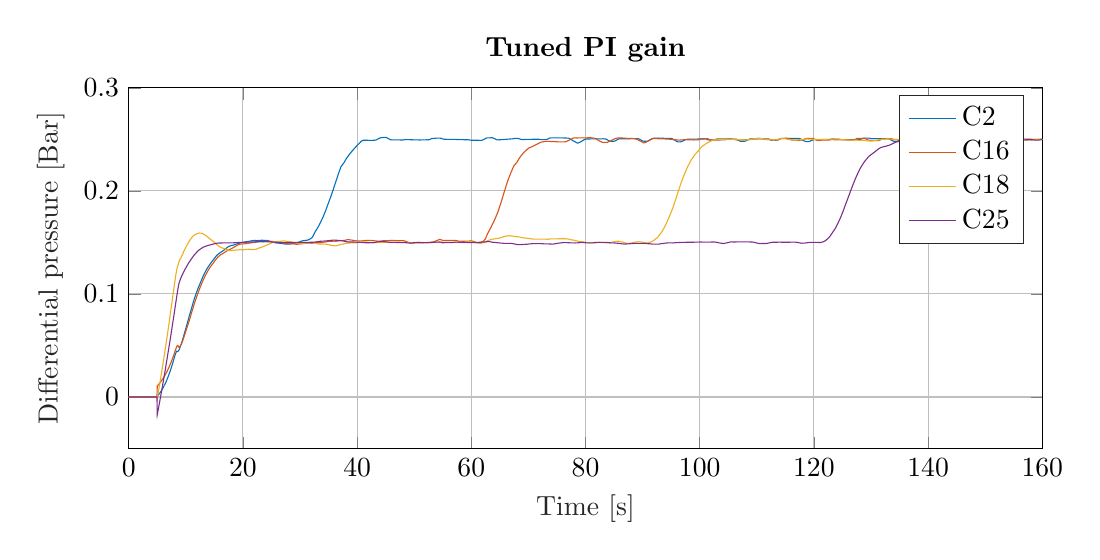
\begin{tikzpicture}

\begin{axis}[%
width=4.568in,
height=1.803in,
at={(0.766in,0.486in)},
scale only axis,
xmin=0,
xmax=160,
xlabel style={font=\color{white!15!black}},
xlabel={Time [s]},
ymin=-0.05,
ymax=0.3,
ylabel style={font=\color{white!15!black}},
ylabel={Differential pressure [Bar]},
axis background/.style={fill=white},
title style={font=\bfseries},
title={Tuned PI gain},
xmajorgrids,
ymajorgrids,
legend style={legend cell align=left, align=left, draw=white!15!black}
]
\addplot [color=mycolor1]
  table[row sep=crcr]{%
0	0\\
4.94999999999999	0\\
5	0.000684261974583933\\
5.5	0.00411168132941953\\
5.80000000000001	0.00671432062560484\\
6.05000000000001	0.00924364613879902\\
6.5	0.014082355816214\\
6.65000000000001	0.0160496089931712\\
7.05000000000001	0.0217925219941435\\
7.40000000000001	0.027346041055722\\
7.65000000000001	0.0317754154447698\\
8	0.0384042033235517\\
8.15000000000001	0.0411351417399715\\
8.34999999999999	0.0440127077223735\\
8.40000000000001	0.0443365102639177\\
8.55000000000001	0.0440188172042895\\
8.59999999999999	0.0441532258064399\\
8.80000000000001	0.04550342130986\\
8.84999999999999	0.0460716031280413\\
9.05000000000001	0.0489980449657992\\
9.34999999999999	0.0539711632453646\\
9.5	0.0567265395894481\\
10.4	0.0742974095796569\\
10.6	0.0783235581622819\\
11.35	0.0927724828934515\\
11.55	0.0963404203323535\\
11.7	0.0986375855327424\\
12.05	0.104026148582591\\
12.35	0.108162267839674\\
12.55	0.110807673509299\\
13	0.116746089931581\\
13.2	0.119214320625616\\
13.45	0.121890273704793\\
13.75	0.124871700879766\\
14.1	0.127779814271747\\
14.45	0.130504643206251\\
15.35	0.136992913000967\\
15.55	0.138019305962843\\
15.9	0.139626099706732\\
16.15	0.140585288367532\\
16.45	0.141611681329437\\
17	0.143811094819171\\
17.35	0.145515640273715\\
17.45	0.145967741935493\\
17.8	0.146713098729236\\
18.05	0.146981915933537\\
18.25	0.147220185728258\\
18.6	0.147898338220926\\
19.05	0.148771994134904\\
19.35	0.149205767350935\\
19.65	0.1497678396872\\
21.05	0.151087487781041\\
21.95	0.151991691104598\\
22.1	0.151930596285439\\
22.3	0.151802297165204\\
22.65	0.15180840664712\\
23.35	0.152126099706749\\
24	0.151845063538616\\
24.3	0.151851173020532\\
24.95	0.150641495601178\\
25.15	0.150256598240475\\
25.35	0.149975562072342\\
25.6	0.1497678396872\\
25.95	0.149395161290329\\
26.1	0.14930351906159\\
26.3	0.149266862170094\\
27.45	0.148411534701864\\
27.7	0.14847873900294\\
27.95	0.148374877810369\\
28.2	0.148484848484856\\
28.6	0.148857526881727\\
29	0.149028592375373\\
29.3	0.149260752688178\\
29.95	0.150568181818187\\
30.4	0.151551808406651\\
30.85	0.151875610948196\\
31.2	0.152126099706749\\
31.45	0.152468230694041\\
31.65	0.152950879765399\\
31.85	0.153616813294235\\
32.15	0.154875366568916\\
32.2	0.155241935483872\\
32.45	0.15796065493646\\
32.65	0.160270039100681\\
33.1	0.164271749755613\\
33.55	0.169006598240458\\
34.05	0.174816715542534\\
34.4	0.179588220918873\\
34.75	0.184872922776151\\
35.15	0.19086021505376\\
35.35	0.193719452590415\\
35.8	0.200995845552285\\
36.75	0.216947702834801\\
37.15	0.22313049853372\\
37.2	0.223723118279565\\
37.45	0.225617057673503\\
37.65	0.226936705767343\\
38.1	0.231237781036157\\
38.5	0.23438416422286\\
39.1	0.238508064516139\\
39.55	0.241379521016626\\
40	0.243976050830895\\
40.7	0.248063294232651\\
40.8	0.24848484848485\\
41.05	0.249150782013686\\
42.7	0.249077468230695\\
43	0.249169110459434\\
43.25	0.249285190615836\\
43.4	0.249645650048876\\
44	0.251435728250243\\
44.35	0.251759530791787\\
44.6	0.251808406647115\\
44.85	0.251942815249265\\
45.1	0.25187561094819\\
45.2	0.251576246334309\\
45.4	0.250879765395894\\
45.85	0.249682306940372\\
46.1	0.249456256109482\\
46.7	0.249566226783969\\
46.95	0.249560117302053\\
47.25	0.249578445747801\\
47.4	0.249529569892474\\
47.7	0.249370723362659\\
48.05	0.249401270772239\\
48.3	0.249828934506354\\
48.5	0.249847262952102\\
50.25	0.249517350928642\\
50.4	0.249566226783969\\
50.9	0.249425708699903\\
52.2	0.249615102639297\\
52.4	0.249584555229717\\
52.6	0.249676197458456\\
52.9	0.250378787878788\\
53.05	0.250818670576734\\
53.3	0.250928641251221\\
53.45	0.250922531769305\\
53.7	0.251111925708699\\
53.85	0.251203567937438\\
54.25	0.251228005865102\\
54.5	0.251191348973606\\
54.7	0.251075268817203\\
55	0.250421554252199\\
55.1	0.250213831867057\\
55.65	0.250073313782991\\
56.6	0.250067204301075\\
58.85	0.249663978494624\\
59.05	0.249657869012708\\
59.4	0.249725073313783\\
60.05	0.249108015640275\\
60.6	0.249169110459434\\
60.85	0.249169110459434\\
61.8	0.249053030303031\\
61.95	0.249297409579668\\
62.7	0.251374633431084\\
62.9	0.251521260997066\\
63.2	0.25151515151515\\
63.7	0.251582355816225\\
63.8	0.251435728250243\\
64.15	0.250519305962854\\
64.4	0.249786168132943\\
64.6	0.249523460410558\\
65.25	0.249725073313783\\
67.2	0.250537634408602\\
67.6	0.250904203323557\\
68.2	0.250971407624633\\
68.35	0.2506903714565\\
68.8	0.249816715542522\\
69	0.249853372434018\\
69.2	0.249871700879766\\
69.5	0.249945014662757\\
70.5	0.250073313782991\\
71.85	0.250128299120234\\
71.95	0.249975562072336\\
72.1	0.249731182795699\\
72.35	0.249725073313783\\
72.75	0.249743401759531\\
73.25	0.249908357771261\\
73.7	0.251282991202345\\
73.95	0.251466275659823\\
75.25	0.25151515151515\\
75.6	0.25151515151515\\
77	0.251234115347017\\
77.1	0.251111925708699\\
77.35	0.250274926686217\\
77.7	0.249101906158359\\
78.55	0.24647482893451\\
78.7	0.24647482893451\\
79.15	0.247623411534704\\
79.75	0.249621212121212\\
79.95	0.250201612903226\\
80.05	0.250397116324535\\
80.65	0.250415444770283\\
81.7	0.250500977517106\\
81.9	0.250604838709677\\
82.2	0.250476539589442\\
83.1	0.250580400782013\\
83.55	0.25036045943304\\
83.8	0.249608993157381\\
84.05	0.248808651026394\\
84.35	0.248081622678427\\
84.5	0.248026637341184\\
85.1	0.248289345063569\\
85.6	0.249798387096803\\
85.8	0.250391006842648\\
85.95	0.250598729227789\\
86.2	0.250592619745873\\
88.8	0.250720918866136\\
88.95	0.25077590420338\\
89.3	0.250519305962911\\
89.45	0.250213831867114\\
89.7	0.249431818181876\\
90.05	0.248350439882756\\
90.3	0.248130498533783\\
90.85	0.248258797654017\\
90.95	0.248448191593411\\
91.15	0.249132453567995\\
91.65	0.250757575757632\\
92	0.251166911045999\\
92.25	0.251203567937495\\
92.6	0.251252443792822\\
92.8	0.25130131964815\\
94.1	0.250946969697026\\
95.05	0.25091031280553\\
95.5	0.249682306940429\\
95.75	0.248906402737106\\
95.95	0.248106060606119\\
96.15	0.247653958944341\\
96.25	0.247617302052845\\
96.45	0.247623411534761\\
96.6	0.24751955034219\\
96.85	0.247916666666725\\
97.25	0.248967497556265\\
97.6	0.249865591397906\\
97.8	0.250097751710712\\
98.3	0.250164956011787\\
99.4	0.250305474095853\\
100.7	0.250427663734172\\
101	0.250629276637397\\
101.2	0.250342130987349\\
101.4	0.249627321603185\\
101.7	0.24942570869996\\
102.5	0.249541788856362\\
102.7	0.249792277614915\\
102.85	0.250097751710712\\
103	0.250476539589499\\
104	0.250476539589499\\
104.45	0.250421554252256\\
104.85	0.250391006842676\\
105.1	0.25041544477034\\
105.95	0.250287145650105\\
106.25	0.250268817204358\\
106.45	0.250128299120291\\
106.65	0.249578445747858\\
107	0.248350439882756\\
107.1	0.248234359726354\\
107.45	0.248222140762522\\
107.6	0.248191593352942\\
107.75	0.248130498533783\\
108.05	0.248429863147663\\
108.4	0.249456256109539\\
108.7	0.250274926686274\\
108.95	0.250391006842676\\
109.95	0.250525415444827\\
110.3	0.250476539589499\\
111.3	0.250470430107583\\
111.85	0.250525415444827\\
112.05	0.25054985337249\\
112.4	0.249499022482951\\
112.5	0.249187438905238\\
112.75	0.249254643206314\\
113	0.249327956989305\\
113.25	0.249193548387154\\
113.65	0.249315738025473\\
113.95	0.250207722385198\\
114.05	0.250543743890574\\
114.25	0.250739247311884\\
114.45	0.25087976539595\\
115.3	0.250965298142773\\
117.5	0.250928641251278\\
117.75	0.250171065493703\\
118	0.249315738025473\\
118.2	0.248765884653039\\
118.5	0.24804496578696\\
118.8	0.247794477028407\\
119.15	0.247861681329482\\
119.6	0.249004154447761\\
120.1	0.249975562072393\\
120.3	0.249871700879822\\
120.8	0.24969452590426\\
121.2	0.249798387096831\\
121.45	0.249871700879822\\
121.9	0.249853372434075\\
122.15	0.249945014662813\\
122.75	0.249902248289402\\
123.25	0.250030547409636\\
124.35	0.249877810361738\\
124.55	0.249828934506411\\
124.85	0.249718963831924\\
127.95	0.249835043988327\\
128.15	0.250091642228796\\
128.45	0.250855327468287\\
128.75	0.251154692082167\\
129.2	0.251209677419411\\
129.5	0.251289100684318\\
129.7	0.251252443792822\\
129.85	0.250995845552353\\
130	0.250708699902304\\
130.3	0.250800342131043\\
130.55	0.250739247311884\\
131.65	0.250720918866136\\
132.3	0.250769794721464\\
132.5	0.250720918866136\\
132.8	0.250812561094875\\
133.05	0.250629276637397\\
133.15	0.250500977517163\\
134.1	0.247776148582659\\
134.3	0.2477150537635\\
134.45	0.247745601173079\\
134.6	0.247696725317752\\
134.75	0.247782258064575\\
135.4	0.24975562072342\\
135.55	0.249981671554309\\
135.65	0.25008553274688\\
136.55	0.249993890518141\\
137.25	0.249975562072393\\
137.9	0.249773949169168\\
138.45	0.249780058651083\\
138.75	0.249780058651083\\
138.9	0.249963343108561\\
139.1	0.250207722385198\\
139.45	0.250207722385198\\
139.95	0.25021994134903\\
140.55	0.250201612903282\\
141.1	0.25008553274688\\
141.85	0.249749511241504\\
142.3	0.249706744868092\\
142.6	0.249847262952159\\
142.8	0.249773949169168\\
143.1	0.249676197458513\\
143.6	0.249523460410614\\
144.1	0.250189393939451\\
144.8	0.250048875855384\\
145.35	0.250006109481973\\
145.8	0.249938905180898\\
146.85	0.250336021505433\\
147.35	0.250274926686274\\
148.65	0.250171065493703\\
149.1	0.249499022482951\\
149.7	0.249663978494681\\
150.45	0.249835043988327\\
150.65	0.250244379276694\\
150.85	0.250488758553331\\
151.1	0.250378787878844\\
152.2	0.250800342131043\\
152.85	0.250769794721464\\
153.3	0.250812561094875\\
153.85	0.2507453567938\\
154.1	0.250311583577769\\
154.75	0.248588709677477\\
155.7	0.248680351906216\\
155.85	0.248930840664769\\
156.1	0.249749511241504\\
156.5	0.24972507331384\\
157	0.249523460410614\\
158	0.249639540567017\\
158.75	0.249786168132999\\
159.6	0.250000000000057\\
159.7	0.250146627566039\\
160.5	0.250079423264964\\
160.7	0.2500549853373\\
};
\addlegendentry{C2}

\addplot [color=mycolor2]
  table[row sep=crcr]{%
0	0\\
4.94999999999999	0\\
5	0.0106182795698828\\
5.25	0.0121700879765285\\
5.90000000000001	0.0169843597263082\\
6.19999999999999	0.0195625610948298\\
6.65000000000001	0.0240285923753731\\
7	0.0280608504398856\\
7.15000000000001	0.030058651026394\\
7.34999999999999	0.0327468230694024\\
7.5	0.0347568426197427\\
7.80000000000001	0.0392778592375294\\
8.30000000000001	0.0472812805474234\\
8.34999999999999	0.0480632942326622\\
8.40000000000001	0.0486803519061709\\
8.55000000000001	0.0500794232649184\\
8.59999999999999	0.0500610948191706\\
8.80000000000001	0.0480510752688303\\
8.84999999999999	0.0480205278592507\\
9.15000000000001	0.0506414956011838\\
9.30000000000001	0.0521627565982499\\
9.5	0.0552969208211209\\
9.80000000000001	0.0602333822091907\\
10.2	0.0672592864125079\\
10.4	0.0705950635386046\\
10.5	0.0723301564027281\\
10.75	0.0768572825024307\\
11.05	0.0824474584555333\\
11.45	0.0897421798631513\\
11.7	0.0939943792766371\\
12.1	0.100219941348968\\
12.5	0.106353861192559\\
12.85	0.111052052785936\\
13.25	0.115957966764427\\
13.45	0.118175708699908\\
13.75	0.121389296187687\\
14.05	0.124211876832845\\
14.3	0.126228005865102\\
14.7	0.129142228738999\\
14.95	0.131133919843592\\
15.2	0.133064516129025\\
15.5	0.135062316715533\\
15.9	0.137261730205267\\
16.15	0.138141495601161\\
16.35	0.138734115347006\\
17.15	0.141648338220932\\
17.45	0.142381476050844\\
18.15	0.144477028348007\\
19.1	0.147507331378307\\
19.45	0.148216031280555\\
19.75	0.148552052785931\\
20.3	0.148631476050838\\
20.65	0.149028592375373\\
20.95	0.149150782013692\\
21.45	0.149645650048882\\
21.7	0.149792277614864\\
22.85	0.150659824046926\\
23.15	0.150708699902253\\
23.7	0.150672043010758\\
23.9	0.150733137829917\\
24.3	0.150898093841647\\
24.75	0.151118035190621\\
25.3	0.150995845552302\\
27.3	0.149407380254161\\
27.65	0.148894183773223\\
27.85	0.148680351906165\\
28.05	0.148552052785931\\
28.7	0.148686461388081\\
29.05	0.148411534701864\\
29.3	0.148228250244387\\
29.6	0.148271016617798\\
31.35	0.149444037145656\\
31.65	0.149327956989254\\
32.05	0.149181329423271\\
32.55	0.149596774193554\\
32.9	0.14993279569893\\
33.05	0.149853372434023\\
33.25	0.149621212121218\\
33.5	0.149639540566966\\
34.2	0.150274926686222\\
34.7	0.150708699902253\\
35	0.15098362658847\\
35.15	0.151050830889545\\
35.55	0.151118035190621\\
35.9	0.151228005865107\\
36.25	0.151099706744873\\
36.7	0.151411290322585\\
36.9	0.151606793743895\\
37.45	0.151759530791793\\
37.7	0.151936705767355\\
37.85	0.152010019550346\\
38.3	0.152675953079182\\
38.6	0.152627077223855\\
39.35	0.151948924731187\\
39.6	0.151710654936466\\
39.75	0.151606793743895\\
39.9	0.151490713587492\\
40.25	0.151484604105576\\
40.55	0.151454056695997\\
40.75	0.151423509286417\\
41.3	0.151790078201373\\
41.75	0.151918377321607\\
42.35	0.152046676441842\\
43.7	0.151154692082116\\
44.85	0.151759530791793\\
45.55	0.151783968719457\\
45.7	0.151857282502448\\
46.1	0.15180840664712\\
46.45	0.151832844574784\\
47.4	0.151728983382213\\
47.8	0.151771749755625\\
48.3	0.151521260997072\\
48.8	0.150452101661784\\
49.05	0.149835043988276\\
49.35	0.149376832844581\\
49.65	0.149297409579674\\
50	0.149480694037152\\
50.2	0.149560117302059\\
50.9	0.149523460410563\\
51.45	0.149584555229723\\
52	0.149859481915939\\
53	0.14982893450636\\
53.25	0.150164956011736\\
54.4	0.152785923753669\\
54.55	0.152785923753669\\
54.65	0.15266373411535\\
54.95	0.152046676441842\\
55.3	0.151845063538616\\
56.75	0.151918377321607\\
57.1	0.151845063538616\\
57.35	0.151820625610952\\
57.5	0.151606793743895\\
57.7	0.151276881720435\\
58.65	0.151160801564032\\
59.15	0.151240224828939\\
59.3	0.151209677419359\\
60.05	0.151490713587492\\
60.2	0.151307429130014\\
60.55	0.150580400782019\\
60.9	0.149890029325519\\
61.2	0.149431818181824\\
61.35	0.149370723362665\\
61.55	0.149725073313789\\
62.1	0.151221896383191\\
62.2	0.151631231671558\\
62.4	0.152908113391987\\
62.45	0.153323558162271\\
62.55	0.154563782991204\\
62.75	0.15723973607038\\
62.9	0.15914589442815\\
63.05	0.160575513196477\\
63.45	0.164693304007812\\
64.05	0.17156647116326\\
64.5	0.177394916911055\\
64.65	0.17953323558163\\
64.8	0.181860948191598\\
65.25	0.189497800586508\\
65.75	0.198723118279588\\
66.15	0.205901759530803\\
66.4	0.210019550342139\\
66.65	0.213697458455528\\
67	0.218542277614858\\
67.3	0.222458455522968\\
67.45	0.224224095796671\\
67.55	0.225012218963855\\
67.95	0.227431573802562\\
68.45	0.232080889540583\\
68.7	0.234023704789848\\
69.3	0.237897116324547\\
69.6	0.239461143695024\\
70.1	0.241678885630506\\
70.35	0.242289833822099\\
70.5	0.242607526881727\\
72.15	0.247140762463346\\
72.7	0.247837243401761\\
72.85	0.247983870967744\\
73	0.24812438905181\\
74.2	0.247941104594332\\
74.6	0.247934995112416\\
75.2	0.247605083088956\\
76	0.24762952101662\\
76.2	0.247580645161293\\
76.35	0.24762952101662\\
76.55	0.247757820136854\\
76.75	0.248173264907138\\
77.85	0.251270772238513\\
78.05	0.251472385141739\\
78.25	0.251411290322579\\
78.45	0.251344086021504\\
78.7	0.251423509286411\\
79.2	0.25148460410557\\
79.45	0.251502932551318\\
80.95	0.251564027370478\\
81.6	0.251130254154447\\
81.8	0.250629276637341\\
82.3	0.24897971652004\\
82.45	0.248478739002934\\
82.95	0.247079667644186\\
83.2	0.247006353861195\\
83.4	0.24710410557185\\
83.85	0.247152981427178\\
84.65	0.249224095796677\\
85.3	0.251038611925708\\
85.65	0.251337976539588\\
86	0.251423509286411\\
86.2	0.251429618768327\\
87.7	0.25082478005865\\
88	0.250940860215053\\
88.55	0.250647605083088\\
88.75	0.250543743890518\\
88.95	0.250171065493646\\
89.2	0.249511241446726\\
90.15	0.246725317693063\\
90.25	0.246584799608996\\
90.45	0.246859726295213\\
91.7	0.250574291300097\\
92.05	0.250873655913978\\
92.35	0.250782013685239\\
93.3	0.250433773216031\\
93.5	0.250507086999022\\
93.9	0.250427663734115\\
94.2	0.250372678396872\\
94.7	0.250183284457478\\
95.25	0.249859481915934\\
95.4	0.24970063538612\\
95.65	0.24967008797654\\
95.95	0.249566226783969\\
96.35	0.249272971652033\\
96.55	0.249309628543529\\
97.25	0.249718963831896\\
97.45	0.249718963831896\\
97.85	0.249694525904232\\
98.5	0.249584555229774\\
98.85	0.249456256109539\\
99.7	0.249468475073371\\
100	0.249981671554309\\
100.2	0.250458211143751\\
100.35	0.250702590420389\\
101.1	0.250635386119313\\
101.4	0.25058040078207\\
101.55	0.250342130987349\\
101.75	0.249657869012765\\
102	0.249431818181876\\
102.3	0.249389051808464\\
102.65	0.24942570869996\\
103.2	0.249456256109539\\
103.5	0.249431818181876\\
103.9	0.249499022482951\\
104.55	0.249682306940429\\
104.7	0.250103861192628\\
105	0.25041544477034\\
106	0.249908357771318\\
106.2	0.249816715542579\\
106.55	0.249382942326548\\
106.8	0.249468475073371\\
108	0.24959066471169\\
108.65	0.249865591397906\\
108.95	0.24992057673515\\
109.2	0.250042766373468\\
109.35	0.250213831867114\\
109.65	0.250604838709734\\
110.15	0.250678152492725\\
110.4	0.250672043010809\\
110.95	0.2507453567938\\
111.6	0.249865591397906\\
112.45	0.24975562072342\\
112.75	0.249645650048933\\
112.95	0.249554007820194\\
113.1	0.249474584555287\\
113.6	0.249517350928699\\
113.75	0.249663978494681\\
114.2	0.250818670576791\\
115.05	0.251111925708756\\
115.25	0.251093597263008\\
115.4	0.250928641251278\\
115.65	0.250525415444827\\
116.05	0.249474584555287\\
116.3	0.249291300097809\\
116.75	0.249272971652061\\
117.05	0.249138563049911\\
117.25	0.249144672531827\\
117.7	0.249242424242482\\
117.95	0.249291300097809\\
118.25	0.249969452590477\\
118.45	0.250488758553331\\
118.7	0.250946969697026\\
118.9	0.250989736070437\\
119.8	0.250873655914035\\
120.5	0.249175219941407\\
120.6	0.24903470185734\\
121.55	0.24926075268823\\
122.65	0.2493646138808\\
122.8	0.249810606060663\\
122.9	0.250103861192628\\
123.15	0.250391006842676\\
124.55	0.250146627566039\\
124.9	0.249541788856362\\
125.05	0.249505131964867\\
125.8	0.249468475073371\\
126.1	0.249334066471221\\
126.5	0.249358504398884\\
127	0.249407380254212\\
127.1	0.249584555229774\\
127.4	0.250519305962911\\
127.55	0.25094086021511\\
127.7	0.250965298142773\\
127.85	0.250867546432119\\
128.35	0.250898093841698\\
128.55	0.250855327468287\\
128.85	0.250861436950203\\
129	0.25071480938422\\
129.2	0.250268817204358\\
129.55	0.249315738025473\\
129.85	0.248973607038181\\
130.55	0.248949169110517\\
130.8	0.248857526881778\\
131.1	0.248906402737106\\
131.25	0.248894183773274\\
131.45	0.249022482893508\\
131.85	0.250152737047955\\
132.1	0.250562072336322\\
132.55	0.250464320625667\\
132.8	0.250727028348052\\
133.5	0.250782013685296\\
134.05	0.249633431085101\\
134.15	0.249535679374446\\
134.85	0.249578445747858\\
135.2	0.249663978494681\\
135.85	0.249896138807486\\
136.05	0.249816715542579\\
136.35	0.250128299120291\\
136.45	0.250323802541601\\
136.65	0.250366568915013\\
137	0.250433773216088\\
137.6	0.250336021505433\\
138	0.250256598240526\\
138.45	0.250024437927721\\
138.7	0.249682306940429\\
138.85	0.249566226784026\\
140.2	0.249615102639353\\
140.45	0.249608993157437\\
140.65	0.249828934506411\\
140.85	0.250421554252256\\
141.15	0.251344086021561\\
141.3	0.251625122189694\\
142.05	0.251655669599273\\
142.25	0.25163123167161\\
142.4	0.251472385141795\\
142.5	0.251325757575813\\
143.1	0.249676197458513\\
143.45	0.248918621700938\\
143.7	0.248949169110517\\
144.2	0.249144672531827\\
144.5	0.249163000977575\\
145.05	0.249584555229774\\
145.6	0.25107526881726\\
145.75	0.251136363636419\\
146.1	0.251124144672588\\
146.45	0.250843108504455\\
146.7	0.250122189638375\\
147.1	0.248930840664769\\
147.25	0.248533724340234\\
147.6	0.248148826979531\\
148	0.248099951124203\\
148.25	0.247996089931632\\
148.55	0.248442082111495\\
149.2	0.250232160312862\\
149.45	0.250965298142773\\
149.8	0.251985581622733\\
149.95	0.252358260019605\\
150.05	0.252382697947269\\
150.3	0.251997800586565\\
150.55	0.251154692082167\\
150.75	0.250604838709734\\
151.4	0.24890029325519\\
152.35	0.248790322580703\\
152.6	0.248912512219022\\
152.9	0.249737292277672\\
153.3	0.250977517106605\\
153.45	0.251246334310906\\
154.5	0.251142473118335\\
154.65	0.250946969697026\\
155.1	0.249615102639353\\
155.3	0.249334066471221\\
155.55	0.24942570869996\\
156	0.249303519061641\\
156.35	0.249272971652061\\
156.6	0.249169110459491\\
157.3	0.2493646138808\\
157.5	0.249615102639353\\
157.6	0.249816715542579\\
157.95	0.249877810361738\\
158.4	0.249767839687252\\
158.8	0.249798387096831\\
160.1	0.249767839687252\\
160.7	0.249743401759588\\
};
\addlegendentry{C16}

\addplot [color=mycolor3]
  table[row sep=crcr]{%
0	0\\
4.94999999999999	0\\
5	-0.0012891006842608\\
5.5	0.0150048875855191\\
5.84999999999999	0.0268572825024478\\
6.25	0.0410129521016529\\
6.65000000000001	0.0556573802541607\\
6.94999999999999	0.0672226295210123\\
7.44999999999999	0.0868523949169173\\
7.75	0.0989980449657821\\
8.15000000000001	0.114839931573812\\
8.19999999999999	0.116654447702842\\
8.40000000000001	0.123258797653961\\
8.44999999999999	0.124578445747801\\
8.84999999999999	0.132050342130981\\
8.90000000000001	0.132704056695985\\
9.09999999999999	0.134457478005857\\
9.19999999999999	0.135538856304976\\
9.40000000000001	0.138031524926674\\
9.75	0.142662512218976\\
9.90000000000001	0.14423264907137\\
10.45	0.149712854349957\\
10.7	0.151979472140766\\
10.85	0.153176930596288\\
11.1	0.155076979472142\\
11.2	0.155816226783969\\
11.35	0.156537145650049\\
11.65	0.157746823069402\\
12.2	0.158907624633429\\
12.35	0.159109237536654\\
12.7	0.158962609970672\\
12.9	0.158657135874876\\
13.25	0.157557429130009\\
13.75	0.155663489736071\\
14.15	0.153824535679377\\
14.7	0.151411290322585\\
14.9	0.150672043010758\\
15.3	0.148619257087006\\
15.55	0.147305718475081\\
15.8	0.146230449657878\\
16.15	0.145075757575768\\
16.55	0.144312072336277\\
17.2	0.143157380254166\\
17.6	0.142198191593366\\
17.85	0.14196603128056\\
18.2	0.142216520039113\\
18.8	0.142613636363649\\
19.25	0.142741935483883\\
19.5	0.143041300097764\\
20	0.142754154447715\\
20.2	0.142949657869025\\
20.5	0.143187927663746\\
21.05	0.143383431085056\\
21.35	0.143139051808419\\
22.05	0.143169599217998\\
22.3	0.143358993157392\\
22.7	0.144342619745856\\
23.3	0.145332355816237\\
23.55	0.14594330400783\\
24.4	0.147825024437935\\
24.55	0.1481182795699\\
24.85	0.149120234604112\\
25.4	0.150543743890523\\
25.55	0.150733137829917\\
25.7	0.150812561094824\\
26	0.150861436950152\\
26.25	0.151001955034218\\
26.5	0.151087487781041\\
27.15	0.151441837732165\\
27.25	0.151447947214081\\
27.65	0.151026392961882\\
28.05	0.15081867057674\\
28.2	0.150763685239497\\
28.5	0.15035434995113\\
28.85	0.149853372434023\\
29.3	0.149315738025422\\
29.5	0.149083577712616\\
29.85	0.148814760508316\\
30	0.148771994134904\\
30.25	0.148686461388081\\
31	0.149535679374395\\
31.2	0.149816715542528\\
31.8	0.149786168132948\\
32.4	0.14946847507332\\
32.55	0.149517350928647\\
32.8	0.149034701857289\\
33.05	0.148820869990232\\
33.25	0.148490957966771\\
34.15	0.148380987292285\\
34.4	0.14841764418378\\
35	0.14778836754644\\
35.45	0.147146871945267\\
36.3	0.146645894428161\\
36.85	0.147568426197466\\
37.35	0.148393206256117\\
37.55	0.148405425219948\\
37.75	0.148802541544484\\
38	0.148991935483878\\
38.15	0.149150782013692\\
38.3	0.149340175953085\\
38.65	0.149419599217993\\
39.45	0.149725073313789\\
39.6	0.149725073313789\\
39.8	0.149670087976546\\
40.25	0.149792277614864\\
40.9	0.150555962854355\\
41.05	0.150617057673514\\
41.65	0.15035434995113\\
42	0.150024437927669\\
42.5	0.149566226783975\\
42.95	0.149627321603134\\
43.5	0.149914467253183\\
43.6	0.149975562072342\\
43.75	0.150006109481922\\
44.25	0.150109970674492\\
44.55	0.149975562072342\\
45.05	0.150164956011736\\
45.25	0.150073313782997\\
45.65	0.149835043988276\\
46.05	0.149865591397855\\
46.4	0.150018328445753\\
46.8	0.150091642228745\\
47.2	0.150226050830895\\
47.65	0.150189393939399\\
47.8	0.150054985337249\\
47.95	0.149938905180846\\
48.3	0.150012218963838\\
48.5	0.149883919843603\\
48.6	0.149780058651032\\
48.9	0.149725073313789\\
49.35	0.14963343108505\\
49.65	0.149474584555236\\
49.8	0.149547898338227\\
50.5	0.150189393939399\\
51.15	0.150073313782997\\
51.4	0.149981671554258\\
51.8	0.149792277614864\\
52	0.149590664711639\\
52.2	0.149572336265891\\
52.45	0.149578445747807\\
52.8	0.149670087976546\\
52.95	0.149957233626594\\
53.5	0.150018328445753\\
53.8	0.150079423264913\\
54.5	0.150195503421315\\
54.75	0.150238269794727\\
55.05	0.150103861192576\\
56.55	0.150018328445753\\
56.75	0.150091642228745\\
57.1	0.149951124144678\\
57.85	0.149926686217015\\
58	0.149908357771267\\
58.2	0.149908357771267\\
58.4	0.1497678396872\\
58.8	0.149896138807435\\
59.05	0.150207722385147\\
59.6	0.150690371456506\\
59.9	0.150641495601178\\
61.15	0.149382942326497\\
61.7	0.149144672531776\\
61.9	0.149425708699908\\
62.55	0.150702590420337\\
62.75	0.151466275659828\\
62.85	0.151716764418381\\
63.15	0.15219941348974\\
63.45	0.152773704789837\\
63.7	0.153201368523952\\
64.2	0.153512952101664\\
64.5	0.153787878787881\\
64.95	0.1541788856305\\
65.15	0.15456989247312\\
65.35	0.154979227761487\\
65.6	0.155382453567938\\
65.85	0.155846774193549\\
66.45	0.156500488758553\\
66.75	0.156378299120234\\
67.65	0.155846774193549\\
67.85	0.155547409579668\\
68.25	0.155406891495602\\
68.35	0.155400782013686\\
68.95	0.154576001955036\\
69.85	0.153934506353863\\
70.1	0.153787878787881\\
70.9	0.153213587487784\\
71.55	0.15315860215054\\
71.95	0.153231915933532\\
72.15	0.153140273704793\\
73.1	0.153128054740961\\
73.4	0.153073069403717\\
73.75	0.153360215053766\\
74.45	0.153402981427178\\
74.65	0.153482404692085\\
74.95	0.153445747800589\\
75.2	0.153494623655916\\
75.55	0.153604594330403\\
76.2	0.153574046920824\\
76.55	0.153537390029328\\
77.1	0.153195259042036\\
77.35	0.15269428152493\\
77.5	0.152535434995116\\
77.85	0.152278836754647\\
78.7	0.151142473118284\\
79.6	0.150464320625616\\
80	0.150036656891501\\
80.65	0.149682306940377\\
81	0.149486803519068\\
82.05	0.149682306940377\\
82.45	0.150171065493652\\
82.6	0.150067204301081\\
82.8	0.149859481915939\\
84.25	0.149456256109488\\
84.55	0.149902248289351\\
84.8	0.150421554252205\\
85.4	0.151032502443798\\
85.8	0.151173020527864\\
86.1	0.150806451612908\\
86.5	0.15035434995113\\
86.85	0.149731182795705\\
87.15	0.149389051808413\\
87.4	0.149010263929625\\
87.6	0.149034701857289\\
88	0.149376832844581\\
88.6	0.150201612903231\\
89.25	0.150641495601178\\
89.5	0.150555962854355\\
89.95	0.150281036168138\\
90.6	0.149486803519068\\
90.85	0.149578445747807\\
91.5	0.150531524926691\\
91.8	0.151411290322585\\
92.1	0.1525293255132\\
92.5	0.154331622678399\\
92.7	0.155449657869013\\
93.25	0.159316959921796\\
93.5	0.161424731182791\\
93.65	0.162921554252193\\
93.95	0.166202346041047\\
94.2	0.169006598240458\\
94.35	0.170845552297152\\
94.95	0.17864736070382\\
95.2	0.182148093841647\\
95.4	0.185184506353863\\
95.65	0.189479472140761\\
95.95	0.194489247311822\\
96.4	0.202168866080143\\
96.85	0.209494134897369\\
97	0.211663000977524\\
97.3	0.215774682306943\\
97.45	0.217986314760509\\
97.7	0.221260997067446\\
98.15	0.226160801564021\\
98.35	0.228329667644175\\
98.55	0.230333577712628\\
99.2	0.235538856304998\\
99.5	0.237353372434029\\
99.75	0.238770772238524\\
100.15	0.241611681329431\\
100.45	0.243255131964816\\
101.05	0.245631720430111\\
101.3	0.246450391006846\\
102.25	0.249163000977518\\
103.05	0.250226050830889\\
103.4	0.250091642228739\\
103.75	0.250177174975562\\
104.05	0.250171065493646\\
104.55	0.250152737047898\\
104.75	0.250219941348973\\
105.05	0.249993890518084\\
105.3	0.250097751710655\\
105.6	0.250042766373411\\
105.85	0.250036656891496\\
107.95	0.249364613880772\\
108.7	0.249914467253234\\
109.1	0.24992057673515\\
110.05	0.251111925708756\\
110.35	0.251093597263008\\
110.55	0.25110581622684\\
111.25	0.250378787878844\\
111.55	0.250128299120291\\
111.85	0.249865591397906\\
112.35	0.249474584555287\\
112.7	0.249584555229774\\
112.85	0.249651759530849\\
113.15	0.249676197458513\\
113.7	0.250067204301132\\
114.1	0.250818670576791\\
114.8	0.250788123167212\\
115.05	0.250470430107583\\
115.45	0.249914467253234\\
116.85	0.249321847507389\\
117.45	0.249712854350008\\
117.75	0.249822825024495\\
118.75	0.25044599217992\\
119.05	0.250164956011787\\
119.3	0.250305474095853\\
119.85	0.250012218963889\\
120.1	0.249981671554309\\
120.6	0.249963343108561\\
120.9	0.249963343108561\\
122.1	0.24969452590426\\
122.5	0.249547898338278\\
123.3	0.249615102639353\\
123.65	0.249382942326548\\
124.45	0.249602883675522\\
124.85	0.249767839687252\\
126.6	0.249211876832902\\
126.85	0.249046920821172\\
127.15	0.249248533724398\\
127.5	0.249376832844632\\
128.1	0.248991935483929\\
128.3	0.249046920821172\\
128.5	0.249150782013743\\
128.75	0.248936950146685\\
128.9	0.248820869990283\\
129.1	0.248771994134955\\
129.4	0.24850928641257\\
130.15	0.248448191593411\\
131.7	0.249859481915991\\
131.9	0.250109970674544\\
132.3	0.250226050830946\\
133.15	0.250464320625667\\
133.6	0.250207722385198\\
133.85	0.250183284457535\\
134	0.250079423264964\\
134.15	0.249993890518141\\
134.4	0.250116080156459\\
134.7	0.249987781036225\\
135.75	0.250397116324592\\
136.05	0.250439882698004\\
136.6	0.250617057673566\\
136.75	0.25058040078207\\
136.95	0.25058040078207\\
137.35	0.25061094819165\\
137.75	0.25061094819165\\
137.95	0.250586510263986\\
138.2	0.25054985337249\\
138.7	0.250433773216088\\
139.3	0.250397116324592\\
139.5	0.25038489736076\\
139.85	0.250531524926743\\
140.5	0.25041544477034\\
140.7	0.250507086999079\\
143.25	0.250397116324592\\
143.5	0.25038489736076\\
144.45	0.250391006842676\\
145.2	0.250134408602207\\
145.45	0.250103861192628\\
145.6	0.2500549853373\\
145.9	0.250109970674544\\
146.45	0.250189393939451\\
146.75	0.250103861192628\\
147.45	0.249688416422345\\
147.8	0.249608993157437\\
148.1	0.24952956989253\\
149	0.249627321603185\\
149.15	0.249706744868092\\
149.35	0.249871700879822\\
149.7	0.249963343108561\\
149.9	0.250109970674544\\
150.45	0.250128299120291\\
150.7	0.250366568915013\\
151.5	0.24989002932557\\
151.8	0.249492913001035\\
152.05	0.249266862170145\\
152.35	0.248863636363694\\
152.65	0.248698680351964\\
152.8	0.248753665689208\\
153.3	0.249059139785004\\
153.55	0.249028592375424\\
153.75	0.249053030303088\\
153.9	0.249108015640331\\
154.15	0.24906524926692\\
156.2	0.248943059628601\\
156.5	0.249059139785004\\
157.5	0.250421554252256\\
157.75	0.250427663734172\\
159.4	0.250103861192628\\
159.6	0.250158846529871\\
159.8	0.25008553274688\\
160.1	0.250030547409636\\
160.45	0.250067204301132\\
160.7	0.250006109481973\\
};
\addlegendentry{C18}

\addplot [color=mycolor4]
  table[row sep=crcr]{%
0	0\\
4.94999999999999	0\\
5	-0.0172165200391134\\
5.19999999999999	-0.0113453079178782\\
5.55000000000001	-0.000788123167154708\\
6	0.0132636852394796\\
6.40000000000001	0.0262035679374435\\
7.34999999999999	0.058681573802545\\
7.94999999999999	0.0804374389051929\\
8.30000000000001	0.0934506353861195\\
8.40000000000001	0.0972018572824993\\
8.59999999999999	0.104191104594321\\
8.65000000000001	0.105761241446714\\
8.80000000000001	0.110080645161304\\
8.84999999999999	0.111186461388087\\
9.25	0.117118768328453\\
9.34999999999999	0.118212365591404\\
9.55000000000001	0.120362903225811\\
9.80000000000001	0.123234359726297\\
10.1	0.126295210166177\\
10.3	0.128189149560114\\
10.5	0.130064760508304\\
10.75	0.132038123167149\\
10.95	0.133809872922768\\
11.45	0.137622189638307\\
11.75	0.139473362658833\\
11.95	0.140676930596271\\
12.1	0.141550586510277\\
12.3	0.142589198435985\\
13.05	0.145393450635396\\
13.4	0.146083822091896\\
13.55	0.146419843597272\\
13.7	0.146731427174984\\
15.25	0.149071358748785\\
15.5	0.149248533724347\\
15.8	0.149444037145656\\
17.9	0.149584555229723\\
18.3	0.149584555229723\\
18.75	0.14979838709678\\
19.85	0.150042766373417\\
20.05	0.150091642228745\\
20.25	0.150079423264913\\
20.95	0.150311583577718\\
21.4	0.150372678396877\\
21.65	0.150470430107532\\
22.1	0.150568181818187\\
22.45	0.150678152492674\\
22.8	0.150745356793749\\
24	0.150708699902253\\
24.15	0.150751466275665\\
24.7	0.150543743890523\\
24.9	0.150445992179868\\
26.95	0.149816715542528\\
28.75	0.149938905180846\\
29.25	0.149938905180846\\
29.55	0.149945014662762\\
31.45	0.150061094819165\\
31.65	0.150103861192576\\
32.05	0.150201612903231\\
32.3	0.150146627565988\\
32.65	0.150366568914961\\
32.85	0.150537634408607\\
33.05	0.150708699902253\\
33.2	0.150757575757581\\
33.5	0.151111925708705\\
34.35	0.151337976539594\\
34.9	0.151661779081138\\
35.65	0.152119990224833\\
35.9	0.152211632453572\\
36.3	0.15213831867058\\
36.8	0.151906158357775\\
37.15	0.151728983382213\\
37.35	0.151619012707727\\
37.65	0.151276881720435\\
37.8	0.151136363636368\\
38.05	0.150733137829917\\
38.25	0.15065371456501\\
38.5	0.150342130987298\\
38.9	0.150464320625616\\
39.2	0.150415444770289\\
40.1	0.150201612903231\\
40.4	0.150171065493652\\
41.3	0.149737292277621\\
41.85	0.149676197458462\\
42	0.149676197458462\\
42.25	0.149731182795705\\
42.6	0.149731182795705\\
42.95	0.149926686217015\\
43.3	0.150287145650054\\
43.6	0.150598729227767\\
44.6	0.150898093841647\\
45.15	0.150482649071364\\
45.8	0.150116080156408\\
46.3	0.150048875855333\\
47.65	0.149841153470192\\
48.25	0.149883919843603\\
48.45	0.149749511241453\\
49.55	0.14930351906159\\
50	0.149908357771267\\
50.3	0.149761730205284\\
50.95	0.149883919843603\\
51.75	0.149761730205284\\
52	0.149773949169116\\
52.75	0.150073313782997\\
52.95	0.150171065493652\\
53.25	0.150146627565988\\
53.6	0.150195503421315\\
53.8	0.150238269794727\\
54.5	0.150372678396877\\
54.7	0.15012829912024\\
54.95	0.149639540566966\\
55.4	0.14979838709678\\
56.3	0.149780058651032\\
56.8	0.149902248289351\\
57.1	0.150213831867063\\
57.45	0.150348240469214\\
58	0.150116080156408\\
58.25	0.150177174975568\\
58.55	0.150207722385147\\
59.35	0.149920576735099\\
59.55	0.14982893450636\\
60.15	0.149890029325519\\
60.3	0.149822825024444\\
62.4	0.150397116324541\\
62.6	0.150659824046926\\
63.05	0.150763685239497\\
63.25	0.150708699902253\\
63.7	0.150164956011736\\
64.25	0.149871700879771\\
64.55	0.149688416422293\\
65.25	0.149297409579674\\
65.5	0.149236314760515\\
65.8	0.149022482893457\\
67	0.149040811339205\\
67.65	0.148393206256117\\
67.8	0.148142717497564\\
68.2	0.147880009775179\\
68.35	0.147800586510272\\
69.8	0.148271016617798\\
70.15	0.148533724340183\\
70.7	0.148759775171072\\
72.2	0.148839198435979\\
72.65	0.148631476050838\\
73.65	0.148509286412519\\
74.3	0.148350439882705\\
75.3	0.149321847507338\\
75.45	0.149395161290329\\
76.1	0.14982893450636\\
76.5	0.149859481915939\\
77.3	0.149590664711639\\
78.3	0.149474584555236\\
78.6	0.149578445747807\\
79.3	0.150067204301081\\
80.1	0.149608993157386\\
81	0.149511241446731\\
81.2	0.149584555229723\\
81.4	0.149651759530798\\
81.7	0.14996334310851\\
82.1	0.150085532746829\\
83.25	0.150067204301081\\
83.45	0.150085532746829\\
84	0.149810606060612\\
84.15	0.149755620723369\\
84.35	0.149584555229723\\
84.75	0.149615102639302\\
85.1	0.149450146627572\\
85.55	0.149217986314767\\
85.8	0.14913856304986\\
86.35	0.148655913978502\\
86.85	0.148387096774201\\
87.45	0.148576490713594\\
87.9	0.148839198435979\\
88.15	0.148900293255139\\
88.9	0.14913856304986\\
89.95	0.149010263929625\\
90.25	0.14913856304986\\
90.45	0.149059139784953\\
90.85	0.148796432062568\\
91.3	0.148668132942333\\
91.65	0.14841764418378\\
91.9	0.148332111436957\\
92.7	0.148307673509294\\
92.9	0.148368768328453\\
93.2	0.14877810361682\\
93.45	0.148881964809391\\
93.6	0.148985826001962\\
93.8	0.149217986314767\\
94.6	0.14960288367547\\
95.1	0.149486803519068\\
95.35	0.149480694037152\\
95.75	0.149712854349957\\
97.05	0.150085532746829\\
97.2	0.150079423264913\\
99.45	0.150238269794727\\
99.65	0.150250488758559\\
100.05	0.150391006842625\\
101.1	0.150268817204307\\
101.5	0.150281036168138\\
102.5	0.150421554252205\\
102.9	0.150164956011736\\
103.2	0.149737292277621\\
103.45	0.149560117302059\\
103.85	0.149150782013692\\
104.15	0.14894305962855\\
104.85	0.14966397849463\\
105.05	0.14996334310851\\
105.45	0.150500977517112\\
105.9	0.150409335288373\\
106.2	0.150397116324541\\
106.45	0.150470430107532\\
106.85	0.150537634408607\\
107.45	0.150513196480944\\
108.5	0.15051930596286\\
109.35	0.150336021505382\\
110.35	0.148991935483878\\
110.5	0.148851417399811\\
111.2	0.148991935483878\\
111.7	0.148967497556214\\
112.1	0.149425708699908\\
112.6	0.150042766373417\\
112.8	0.150195503421315\\
113.45	0.150146627565988\\
113.75	0.150226050830895\\
113.95	0.150281036168138\\
114.55	0.150116080156408\\
116.25	0.150238269794727\\
116.7	0.150305474095802\\
117.9	0.149224095796683\\
118.25	0.14927297165201\\
119.2	0.14996334310851\\
119.9	0.150091642228745\\
121.1	0.149908357771267\\
121.35	0.150140518084072\\
121.7	0.150751466275665\\
121.85	0.151191348973612\\
122.15	0.152297165200395\\
122.35	0.153329667644186\\
122.7	0.155278592375367\\
122.9	0.156647116324535\\
123.8	0.164094574780052\\
124.5	0.172000244379262\\
124.75	0.175305474095779\\
125.2	0.181555474095774\\
125.5	0.186229227761459\\
126.55	0.201771749755579\\
127.1	0.209628543499463\\
127.25	0.211656891495551\\
127.8	0.218487292277587\\
127.95	0.220124633431055\\
128.2	0.222770039100652\\
128.8	0.228030303030295\\
129.2	0.230749022482883\\
129.45	0.232398582600212\\
129.55	0.233052297165216\\
129.9	0.234769061583592\\
130.4	0.236791300097792\\
130.55	0.237347262952142\\
131.3	0.240725806451678\\
131.65	0.241917155425284\\
131.85	0.242350928641315\\
132.2	0.242900782013749\\
132.7	0.243511730205341\\
133.25	0.244428152492731\\
133.7	0.245686705767412\\
135.05	0.249266862170145\\
135.35	0.24956011730211\\
135.55	0.249773949169168\\
137.3	0.250097751710712\\
137.6	0.250262707722442\\
137.8	0.250305474095853\\
138	0.250623167155481\\
138.55	0.250739247311884\\
139.15	0.250836999022539\\
139.35	0.250733137829968\\
140.1	0.250140518084123\\
140.35	0.25025048875861\\
140.55	0.25021994134903\\
140.9	0.250238269794778\\
141.55	0.250189393939451\\
142.2	0.250244379276694\\
142.9	0.249883919843654\\
143.1	0.24952956989253\\
143.4	0.249150782013743\\
143.8	0.2490957966765\\
144	0.249132453567995\\
144.25	0.248949169110517\\
145	0.249926686217066\\
145.15	0.250024437927721\\
145.45	0.250079423264964\\
145.75	0.249951124144729\\
146.1	0.249945014662813\\
147.3	0.249908357771318\\
147.6	0.249914467253234\\
147.85	0.249902248289402\\
148.3	0.250195503421367\\
148.55	0.250409335288424\\
148.8	0.250372678396928\\
149.05	0.250311583577769\\
149.3	0.250507086999079\\
149.55	0.250293255132021\\
149.75	0.250189393939451\\
150.15	0.249431818181876\\
150.5	0.249211876832902\\
151.8	0.249138563049911\\
153.2	0.25061094819165\\
153.5	0.25038489736076\\
153.8	0.25028103616819\\
154.2	0.250012218963889\\
154.4	0.249810606060663\\
154.9	0.249407380254212\\
156.45	0.250103861192628\\
156.65	0.250391006842676\\
157.25	0.250122189638375\\
157.45	0.250006109481973\\
157.8	0.249932795698982\\
158.3	0.249535679374446\\
158.7	0.249407380254212\\
158.9	0.24923020527865\\
159.2	0.249266862170145\\
159.65	0.24959066471169\\
159.85	0.249810606060663\\
160.15	0.249981671554309\\
160.5	0.250134408602207\\
160.7	0.250268817204358\\
};
\addlegendentry{C25}

\end{axis}
\end{tikzpicture}%
% \caption{Step response of one pump PI system.}
% \label{fig:Tikz_NEW_PI_PUMP_GAIN}
% \end{figure}

% Based on the step response shown in \figref{fig:Tikz_NEW_PI_PUMP_GAIN}, it can be concluded that a pressure controller that satisfies the requirements has been found for each pump. 

